\documentclass{article}
\usepackage{amsmath}
\usepackage{amsfonts}
\usepackage[margin=1in]{geometry}
\usepackage{graphicx}
\usepackage{bbm}

\DeclareMathOperator{\Pois}{Pois}
\DeclareMathOperator{\Prob}{P}
\DeclareMathOperator{\Exp}{Exp}
\DeclareMathOperator{\Bernoulli}{Bernoulli}
\DeclareMathOperator{\GammaDist}{Gamma}
\DeclareMathOperator{\NegBin}{NegBin}
\DeclareMathOperator{\Erlang3}{Erlang-3}
\DeclareMathOperator{\E}{E}
\DeclareMathOperator{\Var}{Var}
\DeclareMathOperator{\Cov}{Cov}
\DeclareMathOperator*{\argmax}{\arg\!\max}
\def\bs{\boldsymbol}
\def\ibd{\textrm{IBD}}

\def\H{\mathcal{H}}
\def\R{\mathcal{R}}
\def\X{\bs{X}}
\def\m{\mathrm{(m)}}
\def\p{\mathrm{(p)}}
\def\a{\mathrm{(a)}}
\def\b{\mathrm{(b)}}
\def\P{\mathcal{P}}
\def\U{\mathcal{U}}
\def\ind{\mathbbm{1}}

\begin{document}

\section{General equations}

Define $N(t)$ as the population size at time $t$, with $t$ in units of $2N(0)$.
Let $\lambda(t)$ be the relative population size, scaled by $N(0)$, such that
$N(t) = N(0)\lambda(t)$. Define $\Omega(u,v)$ as the cumulative coalescent rate
between times $u$ and $v$:

\begin{equation}
    \Omega(u,v) = \int_u^v \frac{dt}{\lambda(t)}.
\end{equation}

The state of the TSMC at each point along the genome is described by the vector
$\boldsymbol{s} = (s_3,s_2)$, where $s_3$ is the time of the first coalescence
event and $s_2$ is the time of the second coalescence event amongst the three
lineages in a triploid genome. The equilibrium joint distribution of
$(t_3,t_2)$ is

\begin{equation}
    \pi(t_3,t_2) = \frac{3}{\lambda(t_3)\lambda(t_2)}e^{-3\Omega(0,t_3)}e^{-\Omega(t_3,t_2)}.
    \label{eq:equilibriumjointdistn}
\end{equation}

Let $q(\boldsymbol{t}|\boldsymbol{s})$ be the transition kernel at
recombination sites along the genome. Then

\begin{align}
    \begin{split}
    q(\bs{t}|\bs{s}) &= \\ 
    \intertext{For $t_3=s_3;t_2>s_2$:}
    &\int_0^{s_3}\frac{du}{2s_2+s_3}e^{-3\Omega(u,s_3)}e^{-2\Omega(s_3,s_2)}\frac{1}{\lambda(t_2)}e^{-\Omega(s_2,t_2)}+
    2\int_{s_3}^{s_2}\frac{du}{2s_2+s_3}e^{-2\Omega(u,s_2)}\frac{1}{\lambda(t_2)}e^{-\Omega(s_2,t_2)}\\
    \intertext{For $t_3=s_3;t_2<s_2$:}
    &\int_0^{s_3}\frac{du}{2s_2+s_3}e^{-3\Omega(u,s_3)}\frac{1}{\lambda(t_2)}e^{-2\Omega(s_3,t_2)}+
    2\int_{s_3}^{t_2}\frac{du}{2s_2+s_3}\frac{1}{\lambda(t_2)}e^{-2\Omega(u,t_2)}\\
    \intertext{For $t_3<s_3;t_2=s_3$:}
    &\int_0^{t_3}\frac{du}{2s_2+s_3}e^{-3\Omega(u,t_3)}\frac{2}{\lambda(t_3)}\\
    \intertext{For $t_3<s_3; t_2=s_2$:}
    &2\int_0^{t_3}\frac{du}{2s_2+s_3}\frac{2}{\lambda(t_3)}e^{-3\Omega(u,t_3)}\\
    \intertext{For $t_3>s_3; t_2=s_2$:}
    &2\int_0^{s_3}\frac{du}{2s_2+s_3}e^{-3\Omega(u,s_3)}\frac{2}{\lambda(t_3)}e^{-2\Omega(s_3,t_3)}\\
    \intertext{For $t_3=s_2; t_2>s_2$:}
    &2\int_0^{s_3}\frac{du}{2s_2+s_3}e^{-3\Omega(u,s_3)}e^{-2\Omega(s_3,s_2)}\frac{1}{\lambda(t_2)}e^{-\Omega(s_2,t_2)}
    \intertext{For $t_3=s_3; t_2=s_2$:}
    &3\int_0^{s_3}\frac{du}{2s_2+s_3}\frac{1}{3}\left[1-e^{-3\Omega(u,s_3)}\right]+\int_0^{s_3}\frac{du}{2s_2+s_3}e^{-3\Omega(u,s_3)}\frac{1}{2}\left[1-e^{-2\Omega(s_3,s_2)}\right]+2\int_{s_3}^{s_2}\frac{du}{2s_2+s_3}\frac{1}{2}\left[1-e^{-2\Omega(u,s_2)}\right].
\end{split}
\label{eq:qts}
\end{align}
Each part is implicitly multiplied by a delta function to limit the density to
points where the parameters are assumed to be equal to each other. For example,
the first part of $q(\bs{t}|\bs{s})$ is implicitly multiplied by
$\delta(t_3-s_3)$, and the last part is multiplied by
$\delta(t_3-s_3)\delta(t_2-s_2)$.

\section{Piecewise constant transition probabilities}

Suppose that the population changes size at times $(T_1, \dots, T_n)$ and
that the size between $T_i$ and $T_{i+1}$ is a constant $2N\lambda_i$. Define
$T_0 = 0$, $T_{n+1} = \infty$ and $\Delta_i = T_{i+1}-T_i$. Let $\alpha(t)$ be the index
of the time interval to which $t$ belongs, \emph{i.e.}, $\alpha(t) = \max_i
\{i:T_i \le t\}$.

Then the cumulative coalescent rate between $u$ and $v$ can be written

\begin{equation}
    \Omega(u,v) =
    \begin{cases}
        \frac{v-u}{\lambda_{\alpha(u)}} & \alpha(u) = \alpha(v)\\[1em]
        \frac{T_{\alpha(u)+1}-u}{\lambda_{\alpha(u)}} +
          \sum_{i=\alpha(u)+1}^{\alpha(v)-1}\frac{\Delta_i}{\lambda_i} +
          \frac{v-T_{\alpha(v)}}{\lambda_{\alpha(v)}}
          & \alpha(u) < \alpha(v).
    \end{cases}
\end{equation}
The equilibrium joint density of $(t_3,t_2)$ is now approximately

\begin{equation}
    \pi(t_3,t_2) = \frac{3}{\lambda_{\alpha(t_3)}\lambda_{\alpha(t_2)}}e^{-3\Omega(0,t_3)}e^{-\Omega(t_3,t_2)}.
    \label{eq:marginal}
\end{equation}

There are several integrals of the form $\int_x^y e^{-k\Omega(u,y)}du$ in
Equation \eqref{eq:qts}. This integral can be written

\begin{align}
    \begin{split}
        \int_x^y& e^{-k\Omega(u,y)}du = 
        \int_x^{T_{\alpha(x)+1}} e^{-k\Omega(u,y)}du +
        \sum_{i=\alpha(x)+1}^{\alpha(y)-1}\int_{T_i}^{T_i+1}e^{-k\Omega(u,y)}du +
    \int_{T_\alpha(y)}^y e^{-k\Omega(u,y)}du \\
    &= \int_x^{T_{\alpha(x)+1}} \exp\left(-k\left[\left(T_{\alpha(u)+1}-u\right)\frac{1}{\lambda_{\alpha(u)}} + 
    \sum_{j=\alpha(u)+1}^{\alpha(y)-1}\frac{\Delta_j}{\lambda_j} + (y-T_{\alpha(y)})\frac{1}{\lambda_{\alpha(y)}}
    \right]\right)du + \\
    &\qquad \qquad \sum_{i=\alpha(x)+1}^{\alpha(y)-1}\int_{T_i}^{T_{i+1}}
    \exp\left(-k\left[\left(T_{\alpha(u)+1}-u\right)\frac{1}{\lambda_{\alpha(u)}} + 
    \sum_{j=\alpha(u)+1}^{\alpha(y)-1}\frac{\Delta_j}{\lambda_j} + (y-T_{\alpha(y)})\frac{1}{\lambda_{\alpha(y)}}
    \right]\right)du + \\
    &\qquad \qquad \int_{T_{\alpha(y)}}^y \exp\left(-k(y-u)\frac{1}{\lambda_{\alpha(u)}}\right)du \\
    % subst. appropriate \alpha(x)'s etc. for \alpha(u)
    &= \int_x^{T_{\alpha(x)+1}} \exp\left(-k\left[\left(T_{\alpha(x)+1}-u\right)\frac{1}{\lambda_{\alpha(x)}} + 
    \sum_{j=\alpha(x)+1}^{\alpha(y)-1}\frac{\Delta_j}{\lambda_j} + (y-T_{\alpha(y)})\frac{1}{\lambda_{\alpha(y)}}
    \right]\right)du + \\
    &\qquad \qquad \sum_{i=\alpha(x)+1}^{\alpha(y)-1}\int_{T_i}^{T_{i+1}}
    \exp\left(-k\left[\left(T_{i+1}-u\right)\frac{1}{\lambda_{i}} + 
    \sum_{j=i+1}^{\alpha(y)-1}\frac{\Delta_j}{\lambda_j} + (y-T_{\alpha(y)})\frac{1}{\lambda_{\alpha(y)}}
    \right]\right)du + \\
    &\qquad \qquad \int_{T_{\alpha(y)}}^y \exp\left(-k(y-u)\frac{1}{\lambda_{\alpha(y)}}\right)du \\
    % move constants out of exponent
    &= \exp\left(-k\left[\sum_{j=\alpha(x)+1}^{\alpha(y)-1}\frac{\Delta_j}{\lambda_j} +
        (y-T_{\alpha(y)})\frac{1}{\lambda_{\alpha(y)}}\right]\right) 
        \int_x^{T_{\alpha(x)+1}} \exp\left(-k\left(T_{\alpha(x)+1}-u\right)\frac{1}{\lambda_{\alpha(x)}}\right)du + \\
    &\qquad\qquad \sum_{i=\alpha(x)+1}^{\alpha(y)-1}
        \exp\left(-k\left[\sum_{j=i+1}^{\alpha(y)-1}\frac{\Delta_j}{\lambda_j} + (y-T_{\alpha(y)})\frac{1}{\lambda_{\alpha(y)}}
        \right]\right)
    \int_{T_i}^{T_{i+1}}\exp\left(-k\left(T_{i+1}-u\right)\frac{1}{\lambda_{i}}\right)du + \\
    &\qquad \qquad \int_{T_{\alpha(y)}}^y \exp\left(-k(y-u)\frac{1}{\lambda_{\alpha(y)}}\right)du \\
    % solve integrals
    &= \exp\left(-k\left[\sum_{j=\alpha(x)+1}^{\alpha(y)-1}\frac{\Delta_j}{\lambda_j} +
        (y-T_{\alpha(y)})\frac{1}{\lambda_{\alpha(y)}}\right]\right) 
        \left[1-\exp\left(-\frac{k \left(T_{\alpha(x)+1}-x\right)}{\lambda_{\alpha(x)}}\right)\right]\frac{\lambda_{\alpha(x)}}{k}+\\
    &\qquad\qquad \sum_{i=\alpha(x)+1}^{\alpha(y)-1}
        \exp\left(-k\left[\sum_{j=i+1}^{\alpha(y)-1}\frac{\Delta_j}{\lambda_j} + (y-T_{\alpha(y)})\frac{1}{\lambda_{\alpha(y)}}
        \right]\right)
    \left[1-\exp\left(-\frac{k \Delta_i}{\lambda_i}\right)\right]\frac{\lambda_i}{k}+\\
    &\qquad \qquad 
    \left[1-\exp\left(-\frac{k \left(y-T_{\alpha(y)}\right)}{\lambda_{\alpha(y)}}\right)\right]\frac{\lambda_{\alpha(y)}}{k}\\
    % simplify back to \Omega function notation
    &= \exp\left(-k\Omega(T_{\alpha(x)+1}, y)\right)\left[1-\exp\left(-\frac{k \left(T_{\alpha(x)+1}-x\right)}{\lambda_{\alpha(x)}}\right)\right]\frac{\lambda_{\alpha(x)}}{k}+\\
    &\qquad\qquad \sum_{i=\alpha(x)+1}^{\alpha(y)-1} \exp\big(-k\Omega(T_{i+1},y)\big)
    \left[1-\exp\left(-\frac{k \Delta_i}{\lambda_i}\right)\right]\frac{\lambda_i}{k}+\\
    &\qquad \qquad 
    \left[1-\exp\left(-\frac{k \left(y-T_{\alpha(y)}\right)}{\lambda_{\alpha(y)}}\right)\right]\frac{\lambda_{\alpha(y)}}{k}\\
    % replace exp with e^{}
    &= e^{-k\Omega(T_{\alpha(x)+1}, y)}\left[1-e^{-\frac{k \left(T_{\alpha(x)+1}-x\right)}{\lambda_{\alpha(x)}}}\right]\frac{\lambda_{\alpha(x)}}{k}+
    \sum_{i=\alpha(x)+1}^{\alpha(y)-1} e^{-k\Omega(T_{i+1},y)}
    \left[1-e^{-\frac{k \Delta_i}{\lambda_i}}\right]\frac{\lambda_i}{k}+
    \left[1-e^{-\frac{k \left(y-T_{\alpha(y)}\right)}{\lambda_{\alpha(y)}}}\right]\frac{\lambda_{\alpha(y)}}{k}\\
    % end eqn
    \end{split}
    \label{eq:piecewisenocoalintegral}
\end{align}

With this equation, we can calculate all of the transition probabilities in the
transition kernel \eqref{eq:qts}.

For $t_3=s_3;t_2>s_2$:
    % first summand
\begin{align*}
    &\frac{1}{2s_2+s_3}e^{-2\Omega(s_3,s_2)}\frac{1}{\lambda_{\alpha(t_2)}}e^{-\Omega(s_2,t_2)}
    \left\{\sum_{i=0}^{\alpha(s_3)-1}e^{-3\Omega(T_{i+1},s_3)}
        \left[1-e^{-\frac{3\Delta_i}{\lambda_i}}\right]\frac{\lambda_i}{3}+
    \left[1-e^{-\frac{3\left(s_3-T_{\alpha(s_3)}\right)}{\lambda_{\alpha(s_3)}}}\right]
        \frac{\lambda_{\alpha(s_3)}}{3}\right\}+\\
    % second summand
    &\qquad\frac{2}{2s_2+s_3}\frac{1}{\lambda_{\alpha(t_2)}}e^{-\Omega(s_2,t_2)}\times\\
    &\qquad\Bigg\{e^{-2\Omega(T_{\alpha(s_3)+1},s_2)}\left[1-e^{-\frac{2\left(T_{\alpha(s_3)+1}-s_3\right)}{\lambda_{\alpha(s_3)}}}\right]\frac{\lambda_{\alpha(s_3)}}{2}+\sum_{i=\alpha(s_3)+1}^{\alpha(s_2)-1}e^{-2\Omega\left(T_{i+1},s_2\right)}\left[1-e^{-\frac{2\Delta_i}{\lambda_i}}\right]\frac{\lambda_i}{2}\\
    &\qquad\qquad+\left[1-e^{-\frac{2\left(s_2-T_{\alpha(s_2)}\right)}{\lambda_{\alpha(s_2)}}}\right]\frac{\lambda_{\alpha(s_2)}}{2}
    \Bigg\}
    \\
    % (original)
    &=\int_0^{s_3}\frac{du}{2s_2+s_3}e^{-3\Omega(u,s_3)}e^{-2\Omega(s_3,s_2)}\frac{1}{\lambda(t_2)}e^{-\Omega(s_2,t_2)}+
    2\int_{s_3}^{s_2}\frac{du}{2s_2+s_3}e^{-2\Omega(u,s_2)}\frac{1}{\lambda(t_2)}e^{-\Omega(s_2,t_2)}\\
\end{align*}
For $t_3=s_3; t_2<s_2$:
    % first summand
\begin{align*}
    &\frac{1}{2s_2+s_3}\frac{1}{\lambda_{\alpha(t_2)}}e^{-2\Omega(s_3,t_2)}
    \left\{\sum_{i=0}^{\alpha(s_3)-1}e^{-3\Omega(T_{i+1},s_3)}
        \left[1-e^{-\frac{3\Delta_i}{\lambda_i}}\right]\frac{\lambda_i}{3}+
    \left[1-e^{-\frac{3\left(s_3-T_{\alpha(s_3)}\right)}{\lambda_{\alpha(s_3)}}}\right]
        \frac{\lambda_{\alpha(s_3)}}{3}\right\}+\\
    % second summand
        &\qquad\frac{2}{2s_2+s_3}\frac{1}{\lambda_{\alpha(t_2)}}\\
    &\qquad\Bigg\{e^{-2\Omega(T_{\alpha(s_3)+1},t_2)}\left[1-e^{-\frac{2\left(T_{\alpha(s_3)+1}-s_3\right)}{\lambda_{\alpha(s_3)}}}\right]\frac{\lambda_{\alpha(s_3)}}{2}+\sum_{i=\alpha(s_3)+1}^{\alpha(t_2)-1}e^{-2\Omega\left(T_{i+1},t_2\right)}\left[1-e^{-\frac{2\Delta_i}{\lambda_i}}\right]\frac{\lambda_i}{2}\\
    &\qquad\qquad+\left[1-e^{-\frac{2\left(t_2-T_{\alpha(t_2)}\right)}{\lambda_{\alpha(t_2)}}}\right]\frac{\lambda_{\alpha(t_2)}}{2}
    \Bigg\}\\
    % original
    &=\int_0^{s_3}\frac{du}{2s_2+s_3}e^{-3\Omega(u,s_3)}\frac{1}{\lambda(t_2)}e^{-2\Omega(s_3,t_2)}+
    2\int_{s_3}^{t_2}\frac{du}{2s_2+s_3}\frac{1}{\lambda(t_2)}e^{-2\Omega(u,t_2)}\\
    % for...
\end{align*}
For $t_3<s_3; t_2=s_3$:
\begin{align*}
    &\frac{1}{2s_2+s_3}\frac{2}{\lambda_{\alpha(t_3)}}
    \left\{\sum_{i=0}^{\alpha(t_3)-1}e^{-3\Omega(T_{i+1},t_3)}
        \left[1-e^{-\frac{3\Delta_i}{\lambda_i}}\right]\frac{\lambda_i}{3}+
    \left[1-e^{-\frac{3\left(t_3-T_{\alpha(t_3)}\right)}{\lambda_{\alpha(t_3)}}}\right]
        \frac{\lambda_{\alpha(t_3)}}{3}\right\}\\
    % original
    &=\int_0^{t_3}\frac{du}{2s_2+s_3}e^{-3\Omega(u,t_3)}\frac{2}{\lambda(t_3)}\\
\end{align*}
For $t_3<s_3; t_2=s_2$:
\begin{align*}
    &\frac{2}{2s_2+s_3}\frac{2}{\lambda_{\alpha(t_3)}}
    \left\{\sum_{i=0}^{\alpha(t_3)-1}e^{-3\Omega(T_{i+1},t_3)}
        \left[1-e^{-\frac{3\Delta_i}{\lambda_i}}\right]\frac{\lambda_i}{3}+
    \left[1-e^{-\frac{3\left(t_3-T_{\alpha(t_3)}\right)}{\lambda_{\alpha(t_3)}}}\right]
        \frac{\lambda_{\alpha(t_3)}}{3}\right\}\\
    % original
    &=2\int_0^{t_3}\frac{du}{2s_2+s_3}\frac{2}{\lambda(t_3)}e^{-3\Omega(u,t_3)}\\
    % for...
\end{align*}
For $t_3>s_3; t_2=s_2$:
\begin{align*}
    &\frac{2}{2s_2+s_3}\frac{2}{\lambda_{\alpha(t_3)}}e^{-2\Omega(s_3,t_3)}
    \left\{\sum_{i=0}^{\alpha(s_3)-1}e^{-3\Omega(T_{i+1},s_3)}
        \left[1-e^{-\frac{3\Delta_i}{\lambda_i}}\right]\frac{\lambda_i}{3}+
    \left[1-e^{-\frac{3\left(s_3-T_{\alpha(s_3)}\right)}{\lambda_{\alpha(s_3)}}}\right]
        \frac{\lambda_{\alpha(s_3)}}{3}\right\}\\
    % original
    &=2\int_0^{s_3}\frac{du}{2s_2+s_3}e^{-3\Omega(u,s_3)}\frac{2}{\lambda(t_3)}e^{-2\Omega(s_3,t_3)}\\
\end{align*}
For $t_3=s_2; t_2>s_2$:
\begin{align*}
    &\frac{2}{2s_2+s_3}e^{-2\Omega(s_3,s_2)}\frac{1}{\lambda_{\alpha(t_2)}}e^{-\Omega(s_2,t_2)}
    \left\{\sum_{i=0}^{\alpha(s_3)-1}e^{-3\Omega(T_{i+1},s_3)}
        \left[1-e^{-\frac{3\Delta_i}{\lambda_i}}\right]\frac{\lambda_i}{3}+
    \left[1-e^{-\frac{3\left(s_3-T_{\alpha(s_3)}\right)}{\lambda_{\alpha(s_3)}}}\right]
        \frac{\lambda_{\alpha(s_3)}}{3}\right\}\\
    % original
    &=2\int_0^{s_3}\frac{du}{2s_2+s_3}e^{-3\Omega(u,s_3)}e^{-2\Omega(s_3,s_2)}\frac{1}{\lambda(t_2)}e^{-\Omega(s_2,t_2)}
\end{align*}
For $t_3=s_3; t_2=s_2$:
\begin{align*}
    &\frac{1}{2s_2+s_3}
    \left\{s_3 - \sum_{i=0}^{\alpha(s_3)-1}e^{-3\Omega(T_{i+1},s_3)}
        \left[1-e^{-\frac{3\Delta_i}{\lambda_i}}\right]\frac{\lambda_i}{3}-
    \left[1-e^{-\frac{3\left(s_3-T_{\alpha(s_3)}\right)}{\lambda_{\alpha(s_3)}}}\right]
        \frac{\lambda_{\alpha(s_3)}}{3}\right\}+\\
    &\frac{1}{2s_2+s_3}\frac{1}{2}\left[1-e^{-2\Omega(s_3,s_2)}\right]
    \left\{\sum_{i=0}^{\alpha(s_3)-1}e^{-3\Omega(T_{i+1},s_3)}
        \left[1-e^{-\frac{3\Delta_i}{\lambda_i}}\right]\frac{\lambda_i}{3}+
    \left[1-e^{-\frac{3\left(s_3-T_{\alpha(s_3)}\right)}{\lambda_{\alpha(s_3)}}}\right]
        \frac{\lambda_{\alpha(s_3)}}{3}\right\}+\\
        &\frac{1}{2s_2+s_3}\Bigg[s_2-s_3-e^{-2\Omega(T_{\alpha(s_3)+1},t_2)}\Bigg(1-e^{-\frac{2\left(T_{\alpha(s_3)+1}-s_3\right)}{\lambda_{\alpha(s_3)}}}\Bigg)\frac{\lambda_{\alpha(s_3)}}{2}-\sum_{i=\alpha(s_3)+1}^{\alpha(t_2)-1}e^{-2\Omega\left(T_{i+1},t_2\right)}\Bigg(1-e^{-\frac{2\Delta_i}{\lambda_i}}\Bigg)\frac{\lambda_i}{2}\\
    &\qquad\qquad-\Bigg(1-e^{-\frac{2\left(t_2-T_{\alpha(t_2)}\right)}{\lambda_{\alpha(t_2)}}}\Bigg)\frac{\lambda_{\alpha(t_2)}}{2}
    \Bigg]\\
    \\
    % original
    &=3\int_0^{s_3}\frac{du}{2s_2+s_3}\frac{1}{3}\left[1-e^{-3\Omega(u,s_3)}\right]+\int_0^{s_3}\frac{du}{2s_2+s_3}e^{-3\Omega(u,s_3)}\frac{1}{2}\left[1-e^{-2\Omega(s_3,s_2)}\right]+2\int_{s_3}^{s_2}\frac{du}{2s_2+s_3}\frac{1}{2}\left[1-e^{-2\Omega(u,s_2)}\right].
\end{align*}

\section{Discrete approximation to the triploid SMC' coalescent process}

In order to construct a hidden Markov model (HMM) to infer demography, it is
necessary to discretize the triploid coalescent process described above.

Let the discrete state $(i,j)$, $i<j$, correspond to the continuous states in which ${T_i
< t_3 < T_{i+1}}$ and ${T_j < t_2 < T_{j+1}}$. We first calculate the equilibrium
probability that the coalescent process is in $(i,j)$, assuming $i<j$:

\begin{align}
    \begin{split}
        \pi_{i,j} &=
        \int_{T_i}^{T_{i+1}}\int_{T_j}^{T_{j+1}}\frac{3}{\lambda_i\lambda_j}e^{-3\Omega(0,t_3)}e^{-\Omega(t_3,t_2)}dt_2dt_3\\
        &= \frac{3}{\lambda_i\lambda_j}\int_{T_i}^{T_{i+1}}e^{-3\Omega(0,t_3)}\int_{T_j}^{T_{j+1}}e^{-\Omega(t_3,t_2)}dt_2dt_3\\
        &= \frac{3}{\lambda_i\lambda_j}e^{-3\Omega(0,T_i)}\int_{T_i}^{T_{i+1}}e^{-3\Omega(T_i,t_3)}e^{-\Omega(t_3,T_j)}dt_3
            \int_{T_j}^{T_{j+1}}e^{-\Omega(T_j,t_2)}dt_2\\
        &= \frac{3}{\lambda_i\lambda_j}e^{-3\Omega(0,T_i)}\int_{T_i}^{T_{i+1}}e^{-3\Omega(T_i,t_3)}e^{-\Omega(t_3,T_j)}dt_3
            \int_{T_j}^{T_{j+1}}e^{-\frac{t_2-T_j}{\lambda_j}}dt_2\\
        &= \frac{3}{\lambda_i\lambda_j}e^{-3\Omega(0,T_i)}\lambda_j\left[1-e^{-\frac{\Delta_j}{\lambda_j}}\right]
            \int_{T_i}^{T_{i+1}}e^{-3\Omega(T_i,t_3)}e^{-\Omega(t_3,T_j)}dt_3\\
        &= \frac{3}{\lambda_i\lambda_j}e^{-3\Omega(0,T_i)}\lambda_j\left[1-e^{-\frac{\Delta_j}{\lambda_j}}\right]
            e^{-\Omega(T_{i+1},T_j)}
            \int_{T_i}^{T_{i+1}}e^{-3\Omega(T_i,t_3)}e^{-\Omega(t_3,T_{i+1})}dt_3\\
        &= \frac{3}{\lambda_i\lambda_j}e^{-3\Omega(0,T_i)}\lambda_j\left[1-e^{-\frac{\Delta_j}{\lambda_j}}\right]
            e^{-\Omega(T_{i+1},T_j)}
            \int_{T_i}^{T_{i+1}}e^{-\frac{3(t_3-T_i)}{\lambda_i}}e^{-\frac{T_{i+1}-t_3}{\lambda_i}}dt_3\\
        &= \frac{3}{\lambda_i\lambda_j}e^{-3\Omega(0,T_i)}\lambda_j\left[1-e^{-\frac{\Delta_j}{\lambda_j}}\right]
            e^{-\Omega(T_{i+1},T_j)}
            \frac{\lambda_i}{2} \left(e^{\frac{-\Delta_i}{\lambda_i}}-e^{\frac{-3\Delta_i}{\lambda_i}}\right)\\
        &= \frac{3}{2}e^{-3\Omega(0,T_i)}e^{-\Omega(T_{i+1},T_j)}
            \left(e^{\frac{-\Delta_i}{\lambda_i}}-e^{\frac{-3\Delta_i}{\lambda_i}}\right)
            \left[1-e^{-\frac{\Delta_j}{\lambda_j}}\right].
    \end{split}
    \label{eq:pidiscrete}
\end{align}
If $j=n$, we let $\Delta_j = \infty$ and $1-\exp(-\Delta_j/\lambda_j) = 1$.

It is also necessary to calculate $\pi_{i,i}$:

\begin{align}
    \begin{split}
    \pi_{i,i} &= \int_{T_i}^{T_{i+1}}\int_{t_3}^{T_{i+1}}
    \frac{3}{\lambda_i^2}e^{-3\Omega(0,t_3)}e^{-\Omega(t_3,t_2)}dt_2dt_3\\
    &= \frac{1}{\lambda_i^2}e^{-3\Omega(0,T_i)}\int_{T_i}^{T_{i+1}}
    e^{-3\Omega(T_i,t_3)}\int_{t_3}^{T_{i+1}}e^{-\Omega(t_3,t_2)}dt_2dt_3\\
    &= \frac{3}{\lambda_i^2}e^{-3\Omega(0,T_i)}\int_{T_i}^{T_{i+1}}
    e^{-3\Omega(T_i,t_3)}\int_{t_3}^{T_{i+1}}e^{-\frac{t_2-t_3}{\lambda_i}}dt_2dt_3\\
    &= \frac{3}{\lambda_i^2}e^{-3\Omega(0,T_i)}\int_{T_i}^{T_{i+1}}
    e^{-3\Omega(T_i,t_3)}\left(\lambda_i\left[1-e^{-\frac{T_{i+1}-t_3}{\lambda_i}}\right]\right)dt_3\\
    &= \frac{3}{\lambda_i}e^{-3\Omega(0,T_i)}\int_{T_i}^{T_{i+1}}
    e^{-\frac{3(t_3-T_i)}{\lambda_i}}\left(1-e^{-\frac{T_{i+1}-t_3}{\lambda_i}}\right)dt_3\\
    &= \frac{3}{\lambda_i}e^{-3\Omega(0,T_i)}
    \frac{\lambda_i}{6}\left(2-3e^{-\frac{\Delta_i}{\lambda_i}}+e^{-\frac{3\Delta_i}{\lambda_i}}\right)\\
    &= \frac{1}{2}e^{-3\Omega(0,T_i)}
    \left(2-3e^{-\frac{\Delta_i}{\lambda_i}}+e^{-\frac{3\Delta_i}{\lambda_i}}\right)\\
    \end{split}
\end{align}
For $i = n$, again we let $\Delta_i = \infty$ and thus $\pi_{i,i} = \exp(-3\Omega(0,T_i))$.

Next, we calculate marginal expectations for $t_3$ and $t_2$ given that the
continuous process is in interval represented by $(i,j)$, assuming $i<j$. The
marginal expectation of $t_3$ in the interval $(i,j)$ is 

\begin{align}
    \begin{split}
        \E_{i,j}[t_3] = \E\big[t_3|&t_3 \in [T_i T_{i+1}),t_2 \in [T_j,T_{j+1}) \big]\\
        &= \frac{1}{\pi_{i,j}}\int_{T_i}^{T_{i+1}}\int_{T_j}^{T_{j+1}}t_3\pi(t_3,t_2)dt_2dt_3\\
        &= \frac{1}{\pi_{i,j}}\int_{T_i}^{T_{i+1}}\int_{T_j}^{T_{j+1}}
            \frac{3t_3}{\lambda_i \lambda_j}e^{-3\Omega(0,t_3)}e^{-\Omega(t_3,t_2)}dt_2dt_3\\
        &=\frac{3}{\pi_{i,j}\lambda_i\lambda_j}e^{-3\Omega(0,T_i)}
            \int_{T_i}^{T_{i+1}}t_3e^{-3\Omega(T_i,t_3)}\int_{T_j}^{T_{j+1}}e^{-\Omega(t_3,t_2)}dt_2dt_3\\
        &=\frac{3}{\pi_{i,j}\lambda_i\lambda_j}e^{-3\Omega(0,T_i)}
            \int_{T_i}^{T_{i+1}}t_3e^{-3\Omega(T_i,t_3)}e^{-\Omega(t_3,T_j)}dt_3\int_{T_j}^{T_{j+1}}e^{-\Omega(T_j,t_2)}dt_2\\
        &=\frac{3}{\pi_{i,j}\lambda_i\lambda_j}e^{-3\Omega(0,T_i)}
            \int_{T_i}^{T_{i+1}}t_3e^{-3\Omega(T_i,t_3)}e^{-\Omega(t_3,T_j)}dt_3\int_{T_j}^{T_{j+1}}e^{-\frac{t_2-T_j}{\lambda_j}}dt_2\\
        &=\frac{3}{\pi_{i,j}\lambda_i\lambda_j}e^{-3\Omega(0,T_i)}\lambda_j\left(1-e^{-\frac{\Delta_j}{\lambda_j}}\right)
            \int_{T_i}^{T_{i+1}}t_3e^{-3\Omega(T_i,t_3)}e^{-\Omega(t_3,T_j)}dt_3\\
        &=\frac{3}{\pi_{i,j}\lambda_i\lambda_j}e^{-3\Omega(0,T_i)}
            \lambda_j\left(1-e^{-\frac{\Delta_j}{\lambda_j}}\right)e^{-\Omega(T_{i+1},T_j)}
            \int_{T_i}^{T_{i+1}}t_3e^{-3\Omega(T_i,t_3)}e^{-\Omega(t_3,T_{i+1})}dt_3\\
        &=\frac{3}{\pi_{i,j}\lambda_i\lambda_j}e^{-3\Omega(0,T_i)}
            \lambda_j\left(1-e^{-\frac{\Delta_j}{\lambda_j}}\right)e^{-\Omega(T_{i+1},T_j)}
            \frac{\lambda_i}{4}\left[(\lambda_i+2T_i)e^{\frac{-\Delta_i}{\lambda_i}}-(\lambda_i+2T_{i+1})e^{\frac{-3\Delta_i}{\lambda_i}}\right]\\
        &=\frac{3}{4\pi_{i,j}}e^{-3\Omega(0,T_i)}
            \left(1-e^{-\frac{\Delta_j}{\lambda_j}}\right)e^{-\Omega(T_{i+1},T_j)}
            \left[(\lambda_i+2T_i)e^{\frac{-\Delta_i}{\lambda_i}}-(\lambda_i+2T_{i+1})e^{\frac{-3\Delta_i}{\lambda_i}}\right]\\
    \end{split}
    \label{eq:Et3}
\end{align}
With $j = n$, this is
\begin{align}
    \begin{split}
        \E_{i,j}[t_3] = \E\big[t_3|&t_3 \in [T_i T_{i+1}),t_2 \in [T_n,\infty) \big]\\
        &= \frac{1}{\pi_{i,n}}\int_{T_i}^{T_{i+1}}\int_{T_n}^{\infty}t_3\pi(t_3,t_2)dt_2dt_3\\
        &= \frac{1}{\pi_{i,n}}\int_{T_i}^{T_{i+1}}\int_{T_n}^{\infty}
            \frac{3t_3}{\lambda_i \lambda_n}e^{-3\Omega(0,t_3)}e^{-\Omega(t_3,t_2)}dt_2dt_3\\
        &=\frac{3}{\pi_{i,n}\lambda_i\lambda_n}e^{-3\Omega(0,T_i)}
            \int_{T_i}^{T_{i+1}}t_3e^{-3\Omega(T_i,t_3)}\int_{T_n}^{\infty}e^{-\Omega(t_3,t_2)}dt_2dt_3\\
        &=\frac{3}{\pi_{i,n}\lambda_i\lambda_n}e^{-3\Omega(0,T_i)}
            \int_{T_i}^{T_{i+1}}t_3e^{-3\Omega(T_i,t_3)}e^{-\Omega(t_3,T_n)}dt_3\int_{T_n}^{\infty}e^{-\Omega(T_n,t_2)}dt_2\\
        &=\frac{3}{\pi_{i,n}\lambda_i\lambda_n}e^{-3\Omega(0,T_i)}
            \int_{T_i}^{T_{i+1}}t_3e^{-3\Omega(T_i,t_3)}e^{-\Omega(t_3,T_n)}dt_3\int_{T_n}^{\infty}e^{-\frac{t_2-T_n}{\lambda_n}}dt_2\\
        &=\frac{3}{\pi_{i,n}\lambda_i\lambda_n}e^{-3\Omega(0,T_i)}\lambda_n
            \int_{T_i}^{T_{i+1}}t_3e^{-3\Omega(T_i,t_3)}e^{-\Omega(t_3,T_n)}dt_3\\
        &=\frac{3}{\pi_{i,n}\lambda_i\lambda_n}e^{-3\Omega(0,T_i)}
            \lambda_ne^{-\Omega(T_{i+1},T_n)}
            \int_{T_i}^{T_{i+1}}t_3e^{-3\Omega(T_i,t_3)}e^{-\Omega(t_3,T_{i+1})}dt_3\\
        &=\frac{3}{\pi_{i,n}\lambda_i\lambda_n}e^{-3\Omega(0,T_i)}
            \lambda_ne^{-\Omega(T_{i+1},T_n)}
            \frac{\lambda_i}{4}\left[(\lambda_i+2T_i)e^{\frac{-\Delta_i}{\lambda_i}}-(\lambda_i+2T_{i+1})e^{\frac{-3\Delta_i}{\lambda_i}}\right]\\
        &=\frac{3}{4\pi_{i,n}}e^{-3\Omega(0,T_i)}
            e^{-\Omega(T_{i+1},T_n)}
            \left[(\lambda_i+2T_i)e^{\frac{-\Delta_i}{\lambda_i}}-(\lambda_i+2T_{i+1})e^{\frac{-3\Delta_i}{\lambda_i}}\right]\\
    \end{split}
    \label{eq:Et3}
\end{align}
The marginal expectation of $t_2$ in $(i,j)$ is 
\begin{align}
    \begin{split}
        \E_{i,j}[t_2] = \E\big[t_2|&t_3 \in [T_i T_{i+1}),t_2 \in [T_j,T_{j+1}) \big]\\
        &= \frac{1}{\pi_{i,j}}\int_{T_i}^{T_{i+1}}\int_{T_j}^{T_{j+1}}t_2\pi(t_3,t_2)dt_2dt_3\\
        &= \frac{1}{\pi_{i,j}}\int_{T_i}^{T_{i+1}}\int_{T_j}^{T_{j+1}}
            \frac{3t_2}{\lambda_i \lambda_j}e^{-3\Omega(0,t_3)}e^{-\Omega(t_3,t_2)}dt_2dt_3\\
        &= \frac{3}{\pi_{i,j}\lambda_i\lambda_j}e^{-3\Omega(0,T_i)}e^{-\Omega(T_{i+1},T_j)}
            \int_{T_i}^{T_{i+1}}e^{-3\Omega(T_i,t_3)}e^{-\Omega(t_3,T_{i+1})}dt_3
            \int_{T_j}^{T_{j+1}}t_2e^{-\Omega(T_j,t_2)}dt_2\\
        &= \frac{3}{\pi_{i,j}\lambda_i\lambda_j}e^{-3\Omega(0,T_i)}e^{-\Omega(T_{i+1},T_j)}
            \int_{T_i}^{T_{i+1}}e^{-\frac{3(t_3-T_i)}{\lambda_i}}e^{-\frac{T_{i+1}-t_3}{\lambda_i}}dt_3
            \int_{T_j}^{T_{j+1}}t_2e^{-\Omega(T_j,t_2)}dt_2\\
        &= \frac{3}{\pi_{i,j}\lambda_i\lambda_j}e^{-3\Omega(0,T_i)}e^{-\Omega(T_{i+1},T_j)}
            \frac{\lambda_i}{2} \left(e^{\frac{-\Delta_i}{\lambda_i}}-e^{\frac{-3\Delta_i}{\lambda_i}}\right)
            \int_{T_j}^{T_{j+1}}t_2e^{-\Omega(T_j,t_2)}dt_2\\
        &= \frac{3}{\pi_{i,j}\lambda_i\lambda_j}e^{-3\Omega(0,T_i)}e^{-\Omega(T_{i+1},T_j)}
            \frac{\lambda_i}{2} \left(e^{\frac{-\Delta_i}{\lambda_i}}-e^{\frac{-3\Delta_i}{\lambda_i}}\right)
            \int_{T_j}^{T_{j+1}}t_2e^{-\frac{t_2-T_j}{\lambda_j}}dt_2\\
        &= \frac{3}{\pi_{i,j}\lambda_i\lambda_j}e^{-3\Omega(0,T_i)}e^{-\Omega(T_{i+1},T_j)}
            \frac{\lambda_i}{2} \left(e^{\frac{-\Delta_i}{\lambda_i}}-e^{\frac{-3\Delta_i}{\lambda_i}}\right)
            \lambda_j\left(\lambda_j+T_j-(\lambda_j +T_{j+1}) e^{-\frac{\Delta_j}{\lambda_j}}\right)\\
        &= \frac{3}{2\pi_{i,j}}e^{-3\Omega(0,T_i)}e^{-\Omega(T_{i+1},T_j)}
            \left(e^{\frac{-\Delta_i}{\lambda_i}}-e^{\frac{-3\Delta_i}{\lambda_i}}\right)
            \left(\lambda_j+T_j-(\lambda_j + T_{j+1}) e^{-\frac{\Delta_j}{\lambda_j}}\right).
    \end{split}
    \label{eq:Et2}
\end{align}
With $j=n$, this is 
\begin{align}
    \begin{split}
        \E_{i,n}[t_2] = \E\big[t_2|&t_3 \in [T_i T_{i+1}),t_2 \in [T_n,\infty) \big]\\
        &= \frac{1}{\pi_{i,n}}\int_{T_i}^{T_{i+1}}\int_{T_n}^{\infty}t_2\pi(t_3,t_2)dt_2dt_3\\
        &= \frac{1}{\pi_{i,n}}\int_{T_i}^{T_{i+1}}\int_{T_n}^{\infty}
            \frac{3t_2}{\lambda_i \lambda_n}e^{-3\Omega(0,t_3)}e^{-\Omega(t_3,t_2)}dt_2dt_3\\
        &= \frac{3}{\pi_{i,n}\lambda_i\lambda_n}e^{-3\Omega(0,T_i)}e^{-\Omega(T_{i+1},T_n)}
            \int_{T_i}^{T_{i+1}}e^{-3\Omega(T_i,t_3)}e^{-\Omega(t_3,T_{i+1})}dt_3
            \int_{T_n}^{\infty}t_2e^{-\Omega(T_n,t_2)}dt_2\\
        &= \frac{3}{\pi_{i,n}\lambda_i\lambda_n}e^{-3\Omega(0,T_i)}e^{-\Omega(T_{i+1},T_n)}
            \int_{T_i}^{T_{i+1}}e^{-\frac{3(t_3-T_i)}{\lambda_i}}e^{-\frac{T_{i+1}-t_3}{\lambda_i}}dt_3
            \int_{T_n}^{\infty}t_2e^{-\Omega(T_n,t_2)}dt_2\\
        &= \frac{3}{\pi_{i,n}\lambda_i\lambda_n}e^{-3\Omega(0,T_i)}e^{-\Omega(T_{i+1},T_n)}
            \frac{\lambda_i}{2} \left(e^{\frac{-\Delta_i}{\lambda_i}}-e^{\frac{-3\Delta_i}{\lambda_i}}\right)
            \int_{T_n}^{\infty}t_2e^{-\Omega(T_n,t_2)}dt_2\\
        &= \frac{3}{\pi_{i,n}\lambda_i\lambda_n}e^{-3\Omega(0,T_i)}e^{-\Omega(T_{i+1},T_n)}
            \frac{\lambda_i}{2} \left(e^{\frac{-\Delta_i}{\lambda_i}}-e^{\frac{-3\Delta_i}{\lambda_i}}\right)
            \int_{T_n}^{\infty}t_2e^{-\frac{t_2-T_n}{\lambda_n}}dt_2\\
        &= \frac{3}{\pi_{i,n}\lambda_i\lambda_n}e^{-3\Omega(0,T_i)}e^{-\Omega(T_{i+1},T_n)}
            \frac{\lambda_i}{2} \left(e^{\frac{-\Delta_i}{\lambda_i}}-e^{\frac{-3\Delta_i}{\lambda_i}}\right)
            \lambda_n\left(\lambda_n+T_n\right)\\
        &= \frac{3}{2\pi_{i,n}}e^{-3\Omega(0,T_i)}e^{-\Omega(T_{i+1},T_n)}
             \left(e^{\frac{-\Delta_i}{\lambda_i}}-e^{\frac{-3\Delta_i}{\lambda_i}}\right)
            \left(\lambda_n+T_n\right)\\
    \end{split}
    \label{eq:Et2}
\end{align}

We also calculate the marginal expectations of $s_3$ and $s_2$ conditional on
the interval $(i,i)$:

\begin{align}
    \begin{split}
        \E_{i,i}[t_3] &= \E\big[t_3|t_3 \in [T_i T_{i+1}),t_2 \in [T_i,T_{i+1}) \big]\\
                      &= \frac{1}{\pi_{i,i}}\int_{T_i}^{T_{i+1}}\int_{t_3}^{T_{i+1}}t_3\pi(t_3,t_2)dt_2\,dt_3\\
                      &= \frac{3}{\pi_{i,i}}\int_{T_i}^{T_{i+1}}\int_{t_3}^{T_{i+1}}
                        \frac{t_3}{\lambda_i^2}e^{-3\Omega(0,t_3)}e^{-\Omega(t_3,t_2)}dt_2\,dt_3\\
                      &= \frac{3}{\pi_{i,i}\lambda_i^2}\int_{T_i}^{T_{i+1}}
                        t_3\,e^{-3\Omega(0,t_3)}\int_{t_3}^{T_{i+1}}e^{-\Omega(t_3,t_2)}dt_2\,dt_3\\
                    &= \frac{3}{\pi_{i,i}\lambda_i^2}e^{-3\Omega(0,T_i)}\int_{T_i}^{T_{i+1}}
                        t_3e^{-3\Omega(T_i,t_3)}\int_{t_3}^{T_{i+1}}e^{-\Omega(t_3,t_2)}dt_2\,dt_3\\
                    &= \frac{3}{\pi_{i,i}\lambda_i^2}e^{-3\Omega(0,T_i)}
                        \int_{T_i}^{T_{i+1}}
                        t_3\,e^{-\frac{3(t_3-T_i)}{\lambda_i}}
                        \lambda_i\left(1-e^{-\frac{T_{i+1}-t_3}{\lambda_i}}\right)dt_3\\
                    &= \frac{3}{\pi_{i,i}\lambda_i}e^{-3\Omega(0,T_i)}
                        \int_{T_i}^{T_{i+1}}
                        t_3\,e^{-\frac{3(t_3-T_i)}{\lambda_i}}
                        \left(1-e^{-\frac{T_{i+1}-t_3}{\lambda_i}}\right)dt_3\\
                    &= \frac{3}{\pi_{i,i}\lambda_i}e^{-3\Omega(0,T_i)}
                        \frac{\lambda_i}{36}\left(
                            -9e^{-\frac{\Delta_i}{\lambda_i}}(2T_i+\lambda_i)+4(3T_i+\lambda_i)
                            + e^{-\frac{3\Delta_i}{\lambda_i}}(6T_{i+1}+5\lambda_i)
                        \right)\\
                    &= \frac{1}{12\pi_{i,i}}e^{-3\Omega(0,T_i)}
                        \left(
                            4(3T_i+\lambda_i)
                            + e^{-\frac{3\Delta_i}{\lambda_i}}(6T_{i+1}+5\lambda_i)-9e^{-\frac{\Delta_i}{\lambda_i}}(2T_i+\lambda_i)
                    \right)
    \end{split}
\end{align}
For $i = n$, the expectation is 
\begin{equation}
    \E_{n,n}[s_3] = T_n+\frac{\lambda_n}{3}
\end{equation}
Double-checking:
\begin{align}
    \begin{split}
        \E_{n,n}[t_3] &= \E\big[t_3|t_3 \in [T_n \infty),t_2 \in [T_n,\infty) \big]\\
                      &= \frac{1}{\pi_{n,n}}\int_{T_n}^{\infty}\int_{t_3}^{\infty}t_3\pi(t_3,t_2)dt_2\,dt_3\\
                      &= \frac{3}{\pi_{n,n}\lambda_n^2}\int_{T_n}^{\infty}\int_{t_3}^{\infty}
                        t_3 e^{-3\Omega(0,t_3)}e^{-\Omega(t_3,t_2)}dt_2\,dt_3\\
                      &= \frac{3}{\pi_{n,n}\lambda_n^2}\int_{T_n}^{\infty}
                        t_3 e^{-3\Omega(0,t_3)}\int_{t_3}^{\infty}e^{-\Omega(t_3,t_2)}dt_2\,dt_3\\
                      &= \frac{3}{\pi_{n,n}\lambda_n}\int_{T_n}^{\infty}
                        t_3 e^{-3\Omega(0,t_3)}dt_3\\
                      &= \frac{3}{\pi_{n,n}\lambda_n}e^{-3\Omega(0,T_n)}\int_{T_n}^{\infty}
                        t_3 e^{-3\Omega(T_n,t_3)}dt_3\\
                      &= \frac{3}{\pi_{n,n}\lambda_n}e^{-3\Omega(0,T_n)}\int_{T_n}^{\infty}
                        t_3 e^{-\frac{3(t_3-T_n)}{\lambda_n}}dt_3\\
                      &= \frac{3}{\pi_{n,n}\lambda_n}e^{-3\Omega(0,T_n)}
                        \frac{\lambda_n}{9}(3T_n+\lambda_n)\\
                      &= \frac{1}{3\pi_{n,n}}e^{-3\Omega(0,T_n)}
                        (3T_n+\lambda_n)\\
    \end{split}
\end{align}
Checks out since $\pi_{n,n} = \exp(-3\Omega(0,T_n))$.

\begin{align}
    \begin{split}
        \E_{i,i}[t_2] &= \E\big[t_2|t_3 \in [T_i T_{i+1}),t_2 \in [T_i,T_{i+1}) \big]\\
                      &= \frac{1}{\pi_{i,i}}\int_{T_i}^{T_{i+1}}\int_{t_3}^{T_{i+1}}t_2\pi(t_3,t_2)dt_2\,dt_3\\
                      &= \frac{1}{\pi_{i,i}}\int_{T_i}^{T_{i+1}}\int_{t_3}^{T_{i+1}}
                        \frac{3t_2}{\lambda_i^2}e^{-3\Omega(0,t_3)}e^{-\Omega(t_3,t_2)}dt_2\,dt_3\\
                      &= \frac{3}{\pi_{i,i}\lambda_i^2}\int_{T_i}^{T_{i+1}}\int_{t_3}^{T_{i+1}}
                        t_2\,e^{-3\Omega(0,t_3)}e^{-\Omega(t_3,t_2)}dt_2\,dt_3\\
                      &= \frac{3}{\pi_{i,i}\lambda_i^2}\int_{T_i}^{T_{i+1}}
                        e^{-3\Omega(0,t_3)}\int_{t_3}^{T_{i+1}}t_2\,e^{-\Omega(t_3,t_2)}dt_2\,dt_3\\
                      &= \frac{3}{\pi_{i,i}\lambda_i^2}\int_{T_i}^{T_{i+1}}
                        e^{-3\Omega(0,t_3)}\int_{t_3}^{T_{i+1}}t_2\,e^{-\frac{t_2-t_3}{\lambda_i}}dt_2\,dt_3\\
                      &= \frac{3}{\pi_{i,i}\lambda_i^2}\int_{T_i}^{T_{i+1}}
                        e^{-3\Omega(0,t_3)}\lambda_i\left[(t_3+\lambda_i)-e^{-\frac{T_{i+1}-t_3}{\lambda_i}}(T_{i+1}+\lambda_i)\right]dt_3\\
                        &= \frac{3}{\pi_{i,i}\lambda_i^2}e^{-3\Omega(0,T_i)}\int_{T_i}^{T_{i+1}}
                        e^{-3\Omega(T_i,t_3)}\lambda_i\left[(t_3+\lambda_i)-e^{-\frac{T_{i+1}-t_3}{\lambda_i}}(T_{i+1}+\lambda_i)\right]dt_3\\
                        &= \frac{3}{\pi_{i,i}\lambda_i}e^{-3\Omega(0,T_i)}\int_{T_i}^{T_{i+1}}
                    e^{-\frac{3(t_3-T_i)}{\lambda_i}}\left[(t_3+\lambda_i)-e^{-\frac{T_{i+1}-t_3}{\lambda_i}}(T_{i+1}+\lambda_i)\right]dt_3\\
                        &= \frac{3}{\pi_{i,i}\lambda_i}e^{-3\Omega(0,T_i)}
                                \frac{\lambda_i}{18}\left(e^{-\frac{3\Delta_i}{\lambda_i}}(3T_{i+1}+\lambda_i)
                                + 6T_i + 8\lambda_i - 9e^{-\frac{\Delta_i}{\lambda_i}}(T_{i+1}+\lambda_i)\right)\\
                        &= \frac{1}{6\pi_{i,i}}e^{-3\Omega(0,T_i)}
                                \left(e^{-\frac{3\Delta_i}{\lambda_i}}(3T_{i+1}+\lambda_i)
                                + 6T_i + 8\lambda_i - 9e^{-\frac{\Delta_i}{\lambda_i}}(T_{i+1}+\lambda_i)\right)
                    \\
    \end{split}
\end{align}
For $i=n$, this expectation is 
\begin{equation}
    \E_{n,n}[s_2] = T_n+\frac{\lambda_n}{3}+\lambda_n
\end{equation}

\subsection{Discrete $q\big((k,l)|(i,j)\big)$ transition function}

To calculate the discrete-process transition probabilities from $(i,j)$, to
$(k,l)$, we integrate the transition kernel \eqref{eq:piecewisenocoalintegral}
over the interval corresponding to $(k,l)$, replacing $s_3$ and $s_2$ with
their conditional expectations $\E_{i,j}[s_3]$ and $\E_{i,j}[s_2]$
respectively. Thus

% note to self: another approach would be to evaluate the continuous transition
% kernel at the midpoints (i.e., vector of marginal expectations) of each
% interval, just make the transition probabilities proportional to these.

\begin{equation}
    q\Big((k,l)\,|\,(i,j)\Big) = 
    \int_{T_k}^{T_{k+1}}\int_{T_l}^{T_{l+1}}q\Big((t_3,t_2)|\left(\E_{i,j}[s_3],\E_{i,j}[s_2]\right)\Big)dt_2dt_3.
\end{equation}
Note that in any single transition, either the first or second coalescence time
changes, but not both. This simplifies the calculation of these integrals.

% discrete transitions
\subsubsection{Case A}
For $i=k< j<l$, ($t_3=s_3\,;t_2>s_2$):
    % first summand
\begin{align*}
    % from above
    &=\frac{1}{2s_2+s_3}e^{-2\Omega(s_3,s_2)}\frac{1}{\lambda_{\alpha(t_2)}}e^{-\Omega(s_2,t_2)}
    \left\{\sum_{i=0}^{\alpha(s_3)-1}e^{-3\Omega(T_{i+1},s_3)}
        \left[1-e^{-\frac{3\Delta_i}{\lambda_i}}\right]\frac{\lambda_i}{3}+
    \left[1-e^{-\frac{3\left(s_3-T_{\alpha(s_3)}\right)}{\lambda_{\alpha(s_3)}}}\right]
        \frac{\lambda_{\alpha(s_3)}}{3}\right\}+\\
    &\qquad\frac{2}{2s_2+s_3}\frac{1}{\lambda_{\alpha(t_2)}}e^{-\Omega(s_2,t_2)}\times\\
    &\qquad\Bigg\{e^{-2\Omega(T_{\alpha(s_3)+1},s_2)}\left[1-e^{-\frac{2\left(T_{\alpha(s_3)+1}-s_3\right)}{\lambda_{\alpha(s_3)}}}\right]\frac{\lambda_{\alpha(s_3)}}{2}+\sum_{i=\alpha(s_3)+1}^{\alpha(s_2)-1}e^{-2\Omega\left(T_{i+1},s_2\right)}\left[1-e^{-\frac{2\Delta_i}{\lambda_i}}\right]\frac{\lambda_i}{2}\\
    &\qquad\qquad+\left[1-e^{-\frac{2\left(s_2-T_{\alpha(s_2)}\right)}{\lambda_{\alpha(s_2)}}}\right]\frac{\lambda_{\alpha(s_2)}}{2}
    \Bigg\}
    \\
    % discrete
    &=\int_{T_k}^{T_{k+1}}\int_{T_l}^{T_{l+1}}\frac{1}{2\E_{i,j}[s_2]+\E_{i,j}[s_3]}e^{-2\Omega(\E_{i,j}[s_3],\E_{i,j}[s_2])}\frac{1}{\lambda_l}e^{-\Omega(\E_{i,j}[s_2],t_2)}\times\\
    &\qquad\left\{\sum_{a=0}^{i-1}e^{-3\Omega(T_{a+1},\E_{i,j}[s_3])}
        \left[1-e^{-\frac{3\Delta_a}{\lambda_a}}\right]\frac{\lambda_a}{3}+
    \left[1-e^{-\frac{3\left(\E_{i,j}[s_3]-T_i\right)}{\lambda_i}}\right]
    \frac{\lambda_i}{3}\right\}\delta(t_3-s_3)dt_2dt_3+\\
    &\qquad\int_{T_k}^{T_{k+1}}\int_{T_l}^{T_{l+1}}
        \frac{2}{2\E_{i,j}[s_2]+\E_{i,j}[s_3]}\frac{1}{\lambda_l}e^{-\Omega(\E_{i,j}[s_2],t_2)}\times\\
    &\qquad\Bigg\{e^{-2\Omega(T_{i+1},\E_{i,j}[s_2])}\left[1-e^{-\frac{2\left(T_{i+1}-\E_{i,j}[s_3]\right)}{\lambda_i}}\right]\frac{\lambda_i}{2}+\sum_{a=i+1}^{j-1}e^{-2\Omega\left(T_{a+1},\E_{i,j}[s_2]\right)}\left[1-e^{-\frac{2\Delta_a}{\lambda_a}}\right]\frac{\lambda_a}{2}+\\
    &\qquad\qquad\left[1-e^{-\frac{2\left(\E_{i,j}[s_2]-T_j\right)}{\lambda_j}}\right]\frac{\lambda_j}{2}
    \Bigg\}\delta(t_3-s_3)dt_2dt_3\\
    \\
    % discrete simplified
    &=\int_{T_l}^{T_{l+1}}\frac{1}{2\E_{i,j}[s_2]+\E_{i,j}[s_3]}e^{-2\Omega(\E_{i,j}[s_3],\E_{i,j}[s_2])}\frac{1}{\lambda_l}e^{-\Omega(\E_{i,j}[s_2],t_2)}\times\\
    &\qquad\left\{\sum_{a=0}^{i-1}e^{-3\Omega(T_{a+1},\E_{i,j}[s_3])}
        \left[1-e^{-\frac{3\Delta_a}{\lambda_a}}\right]\frac{\lambda_a}{3}+
    \left[1-e^{-\frac{3\left(\E_{i,j}[s_3]-T_i\right)}{\lambda_i}}\right]
    \frac{\lambda_i}{3}\right\}dt_2+\\
    &\qquad\int_{T_l}^{T_{l+1}}
        \frac{2}{2\E_{i,j}[s_2]+\E_{i,j}[s_3]}\frac{1}{\lambda_l}e^{-\Omega(\E_{i,j}[s_2],t_2)}\times\\
    &\qquad\Bigg\{e^{-2\Omega(T_{i+1},\E_{i,j}[s_2])}\left[1-e^{-\frac{2\left(T_{i+1}-\E_{i,j}[s_3]\right)}{\lambda_i}}\right]\frac{\lambda_i}{2}+\sum_{a=i+1}^{j-1}e^{-2\Omega\left(T_{a+1},\E_{i,j}[s_2]\right)}\left[1-e^{-\frac{2\Delta_a}{\lambda_a}}\right]\frac{\lambda_a}{2}+\\
    &\qquad\qquad\left[1-e^{-\frac{2\left(\E_{i,j}[s_2]-T_j\right)}{\lambda_j}}\right]\frac{\lambda_j}{2}
    \Bigg\}dt_2\\
    \\
    % moving integral
    &=\frac{1}{2\E_{i,j}[s_2]+\E_{i,j}[s_3]}e^{-2\Omega(\E_{i,j}[s_3],\E_{i,j}[s_2])}\frac{1}{\lambda_l}\times\\
    &\qquad\left\{\sum_{a=0}^{i-1}e^{-3\Omega(T_{a+1},\E_{i,j}[s_3])}
        \left[1-e^{-\frac{3\Delta_a}{\lambda_a}}\right]\frac{\lambda_a}{3}+
    \left[1-e^{-\frac{3\left(\E_{i,j}[s_3]-T_i\right)}{\lambda_i}}\right]
    \frac{\lambda_i}{3}\right\}\int_{T_l}^{T_{l+1}}e^{-\Omega(\E_{i,j}[s_2],t_2)}dt_2+\\
    % second integral / summand
    &\qquad
        \frac{2}{2\E_{i,j}[s_2]+\E_{i,j}[s_3]}\frac{1}{\lambda_l}\Bigg\{e^{-2\Omega(T_{i+1},\E_{i,j}[s_2])}\left[1-e^{-\frac{2\left(T_{i+1}-\E_{i,j}[s_3]\right)}{\lambda_i}}\right]\frac{\lambda_i}{2}+\\
    &\qquad\sum_{a=i+1}^{j-1}e^{-2\Omega\left(T_{a+1},\E_{i,j}[s_2]\right)}\left[1-e^{-\frac{2\Delta_a}{\lambda_a}}\right]\frac{\lambda_a}{2}+
            \left[1-e^{-\frac{2\left(\E_{i,j}[s_2]-T_j\right)}{\lambda_j}}\right]\frac{\lambda_j}{2}
    \Bigg\}\int_{T_l}^{T_{l+1}}e^{-\Omega(\E_{i,j}[s_2],t_2)}dt_2\\
    \displaybreak
    % --- simplifying integral ---
    &=\frac{1}{2\E_{i,j}[s_2]+\E_{i,j}[s_3]}e^{-2\Omega(\E_{i,j}[s_3],\E_{i,j}[s_2])}\frac{1}{\lambda_l}\times\\
    &\qquad\left\{\sum_{a=0}^{i-1}e^{-3\Omega(T_{a+1},\E_{i,j}[s_3])}
        \left[1-e^{-\frac{3\Delta_a}{\lambda_a}}\right]\frac{\lambda_a}{3}+
    \left[1-e^{-\frac{3\left(\E_{i,j}[s_3]-T_i\right)}{\lambda_i}}\right]
    \frac{\lambda_i}{3}\right\}
    e^{-\Omega(\E_{i,j}[s_2], T_l)}\int_{T_l}^{T_{l+1}}e^{-\Omega(T_l,t_2)}dt_2+\\
    % (second integral / summand)
    &\qquad
        \frac{2}{2\E_{i,j}[s_2]+\E_{i,j}[s_3]}\frac{1}{\lambda_l}\Bigg\{e^{-2\Omega(T_{i+1},\E_{i,j}[s_2])}\left[1-e^{-\frac{2\left(T_{i+1}-\E_{i,j}[s_3]\right)}{\lambda_i}}\right]\frac{\lambda_i}{2}+\\
    &\qquad\sum_{a=i+1}^{j-1}e^{-2\Omega\left(T_{a+1},\E_{i,j}[s_2]\right)}\left[1-e^{-\frac{2\Delta_a}{\lambda_a}}\right]\frac{\lambda_a}{2}+
            \left[1-e^{-\frac{2\left(\E_{i,j}[s_2]-T_j\right)}{\lambda_j}}\right]\frac{\lambda_j}{2}
    \Bigg\}
    e^{-\Omega(\E_{i,j}[s_2], T_l)}\int_{T_l}^{T_{l+1}}e^{-\Omega(T_l,t_2)}dt_2+\\
    % simplifying integrals 2
    &=\frac{1}{2\E_{i,j}[s_2]+\E_{i,j}[s_3]}e^{-2\Omega(\E_{i,j}[s_3],\E_{i,j}[s_2])}\frac{1}{\lambda_l}\times\\
    &\qquad\left\{\sum_{a=0}^{i-1}e^{-3\Omega(T_{a+1},\E_{i,j}[s_3])}
        \left[1-e^{-\frac{3\Delta_a}{\lambda_a}}\right]\frac{\lambda_a}{3}+
    \left[1-e^{-\frac{3\left(\E_{i,j}[s_3]-T_i\right)}{\lambda_i}}\right]
    \frac{\lambda_i}{3}\right\}
    e^{-\Omega(\E_{i,j}[s_2], T_l)}\int_{T_l}^{T_{l+1}}e^{-\frac{t_2-T_l}{\lambda_l}}dt_2+\\
    % (second integral / summand)
    &\qquad
        \frac{2}{2\E_{i,j}[s_2]+\E_{i,j}[s_3]}\frac{1}{\lambda_l}\Bigg\{e^{-2\Omega(T_{i+1},\E_{i,j}[s_2])}\left[1-e^{-\frac{2\left(T_{i+1}-\E_{i,j}[s_3]\right)}{\lambda_i}}\right]\frac{\lambda_i}{2}+\\
    &\qquad\sum_{a=i+1}^{j-1}e^{-2\Omega\left(T_{a+1},\E_{i,j}[s_2]\right)}\left[1-e^{-\frac{2\Delta_a}{\lambda_a}}\right]\frac{\lambda_a}{2}+
            \left[1-e^{-\frac{2\left(\E_{i,j}[s_2]-T_j\right)}{\lambda_j}}\right]\frac{\lambda_j}{2}
    \Bigg\}
    e^{-\Omega(\E_{i,j}[s_2], T_l)}\int_{T_l}^{T_{l+1}}e^{-\frac{t_2-T_l}{\lambda_l}}dt_2\\
    % solving integrals, final answer
    &=\frac{1}{2\E_{i,j}[s_2]+\E_{i,j}[s_3]}e^{-2\Omega(\E_{i,j}[s_3],\E_{i,j}[s_2])}\frac{1}{\lambda_l}\times\\
    &\qquad\left\{\sum_{a=0}^{i-1}e^{-3\Omega(T_{a+1},\E_{i,j}[s_3])}
        \left[1-e^{-\frac{3\Delta_a}{\lambda_a}}\right]\frac{\lambda_a}{3}+
    \left[1-e^{-\frac{3\left(\E_{i,j}[s_3]-T_i\right)}{\lambda_i}}\right]
    \frac{\lambda_i}{3}\right\}
    e^{-\Omega(\E_{i,j}[s_2], T_l)}\lambda_l\left(1-e^{-\frac{\Delta_l}{\lambda_l}}\right)+\\
    % (second integral / summand)
    &\qquad
        \frac{2}{2\E_{i,j}[s_2]+\E_{i,j}[s_3]}\frac{1}{\lambda_l}\Bigg\{e^{-2\Omega(T_{i+1},\E_{i,j}[s_2])}\left[1-e^{-\frac{2\left(T_{i+1}-\E_{i,j}[s_3]\right)}{\lambda_i}}\right]\frac{\lambda_i}{2}+\\
    &\qquad\sum_{a=i+1}^{j-1}e^{-2\Omega\left(T_{a+1},\E_{i,j}[s_2]\right)}\left[1-e^{-\frac{2\Delta_a}{\lambda_a}}\right]\frac{\lambda_a}{2}+
            \left[1-e^{-\frac{2\left(\E_{i,j}[s_2]-T_j\right)}{\lambda_j}}\right]\frac{\lambda_j}{2}
    \Bigg\}
    e^{-\Omega(\E_{i,j}[s_2], T_l)}\lambda_l\left(1-e^{-\frac{\Delta_l}{\lambda_l}}\right)\\
\end{align*}
Here we assume that $\Delta_n = \infty$ and thus $e^{-\Delta_n/\lambda_n} = 0$.

\subsubsection{Case B}
For $i=k<l<j$ ($t_3=s_3; t_2<s_2$): % (i,j) -> (k,l)   (s_3,s_2) -> (t_3, t_2)
\begin{align*}
    % original, with sum indices replaced by a
    &=\int_{T_k}^{T_{k+1}}\int_{T_l}^{T_{l+1}}\frac{1}{2s_2+s_3}\frac{1}{\lambda_{\alpha(t_2)}}e^{-2\Omega(s_3,t_2)}\\
    &\qquad\left\{\sum_{a=0}^{\alpha(s_3)-1}e^{-3\Omega(T_{a+1},s_3)}
        \left[1-e^{-\frac{3\Delta_a}{\lambda_a}}\right]\frac{\lambda_a}{3}+
    \left[1-e^{-\frac{3\left(s_3-T_{\alpha(s_3)}\right)}{\lambda_{\alpha(s_3)}}}\right]
        \frac{\lambda_{\alpha(s_3)}}{3}\right\}\delta(t_3-s_3)dt_2dt_3+\\
        &\int_{T_k}^{T_{k+1}}\int_{T_l}^{T_{l+1}}\frac{2}{2s_2+s_3}\frac{1}{\lambda_{\alpha(t_2)}}\\
    &\qquad\Bigg\{e^{-2\Omega(T_{\alpha(s_3)+1},t_2)}\left[1-e^{-\frac{2\left(T_{\alpha(s_3)+1}-s_3\right)}{\lambda_{\alpha(s_3)}}}\right]\frac{\lambda_{\alpha(s_3)}}{2}+\sum_{a=\alpha(s_3)+1}^{\alpha(t_2)-1}e^{-2\Omega\left(T_{a+1},t_2\right)}\left[1-e^{-\frac{2\Delta_a}{\lambda_a}}\right]\frac{\lambda_a}{2}\\
    &\qquad\qquad+\left[1-e^{-\frac{2\left(t_2-T_{\alpha(t_2)}\right)}{\lambda_{\alpha(t_2)}}}\right]\frac{\lambda_{\alpha(t_2)}}{2}
    \Bigg\}\delta(t_3-s_3)dt_2dt_3\\[2em]
    % replace alphas and s_3's, s_2's
    &=\int_{T_l}^{T_{l+1}}\frac{1}{2\E_{i,j}[s_2]+\E_{i,j}[s_3]}\frac{1}{\lambda_l}e^{-2\Omega(\E_{i,j}[s_3],t_2)}\\
    &\qquad\left\{\sum_{a=0}^{i-1}e^{-3\Omega(T_{a+1},\E_{i,j}[s_3])}
        \left[1-e^{-\frac{3\Delta_a}{\lambda_a}}\right]\frac{\lambda_a}{3}+
    \left[1-e^{-\frac{3\left(\E_{i,j}[s_3]-T_{i}\right)}{\lambda_{i}}}\right]
        \frac{\lambda_{i}}{3}\right\}dt_2+\\
        &\int_{T_l}^{T_{l+1}}\frac{2}{2\E_{i,j}[s_2]+\E_{i,j}[s_3]}\frac{1}{\lambda_{l}}\\
    &\qquad\Bigg\{e^{-2\Omega(T_{i+1},t_2)}\left[1-e^{-\frac{2\left(T_{i+1}-\E_{i,j}[s_3]\right)}{\lambda_{i}}}\right]\frac{\lambda_{i}}{2}+\sum_{a=i+1}^{l-1}e^{-2\Omega\left(T_{a+1},t_2\right)}\left[1-e^{-\frac{2\Delta_a}{\lambda_a}}\right]\frac{\lambda_a}{2}\\
    &\qquad\qquad+\left[1-e^{-\frac{2\left(t_2-T_{l}\right)}{\lambda_{l}}}\right]\frac{\lambda_{l}}{2}
    \Bigg\}dt_2\\[2em]
    % move the integrals
    &=\frac{1}{2\E_{i,j}[s_2]+\E_{i,j}[s_3]}\frac{1}{\lambda_l}\\
    &\qquad\left\{\sum_{a=0}^{i-1}e^{-3\Omega(T_{a+1},\E_{i,j}[s_3])}
    \left[1-e^{-\frac{3\Delta_a}{\lambda_a}}\right]\frac{\lambda_a}{3}+
    \left[1-e^{-\frac{3\left(\E_{i,j}[s_3]-T_{i}\right)}{\lambda_{i}}}\right]
    \frac{\lambda_{i}}{3}\right\}
    \int_{T_l}^{T_{l+1}}e^{-2\Omega(\E_{i,j}[s_3],t_2)}dt_2+\\
    &\int_{T_l}^{T_{l+1}}
    \frac{2}{2\E_{i,j}[s_2]+\E_{i,j}[s_3]}\frac{1}{\lambda_{l}}
    \left(e^{-2\Omega(T_{i+1},t_2)}\left[1-e^{-\frac{2\left(T_{i+1}-\E_{i,j}[s_3]\right)}{\lambda_{i}}}\right]
    \frac{\lambda_{i}}{2}\right)dt_2+\\
    &\int_{T_l}^{T_{l+1}}\frac{2}{2\E_{i,j}[s_2]+\E_{i,j}[s_3]}\frac{1}{\lambda_{l}}
    \left(\sum_{a=i+1}^{l-1}e^{-2\Omega\left(T_{a+1},t_2\right)}
    \left[1-e^{-\frac{2\Delta_a}{\lambda_a}}\right]\frac{\lambda_a}{2}\right)dt_2+\\
    &\int_{T_l}^{T_{l+1}}\frac{2}{2\E_{i,j}[s_2]+\E_{i,j}[s_3]}\frac{1}{\lambda_{l}}
    \left[1-e^{-\frac{2\left(t_2-T_{l}\right)}{\lambda_{l}}}\right]\frac{\lambda_{l}}{2}dt_2\\
    % move the integrals
    &=\frac{1}{2\E_{i,j}[s_2]+\E_{i,j}[s_3]}\frac{1}{\lambda_l}\\
    &\qquad\left\{\sum_{a=0}^{i-1}e^{-3\Omega(T_{a+1},\E_{i,j}[s_3])}
    \left[1-e^{-\frac{3\Delta_a}{\lambda_a}}\right]\frac{\lambda_a}{3}+
    \left[1-e^{-\frac{3\left(\E_{i,j}[s_3]-T_{i}\right)}{\lambda_{i}}}\right]
    \frac{\lambda_{i}}{3}\right\}\int_{T_l}^{T_{l+1}}e^{-2\Omega(\E_{i,j}[s_3],t_2)}dt_2+\\
    &\frac{2}{2\E_{i,j}[s_2]+\E_{i,j}[s_3]}\frac{1}{\lambda_{l}}
    \left(\left[1-e^{-\frac{2\left(T_{i+1}-\E_{i,j}[s_3]\right)}{\lambda_{i}}}\right]
    \frac{\lambda_{i}}{2}\right)\int_{T_l}^{T_{l+1}}e^{-2\Omega(T_{i+1},t_2)}dt_2+\\
    \displaybreak
    &\int_{T_l}^{T_{l+1}}\frac{2}{2\E_{i,j}[s_2]+\E_{i,j}[s_3]}\frac{1}{\lambda_{l}}
    \left(\sum_{a=i+1}^{l-1}e^{-2\Omega\left(T_{a+1},t_2\right)}
    \left[1-e^{-\frac{2\Delta_a}{\lambda_a}}\right]\frac{\lambda_a}{2}\right)dt_2+\\
    &\frac{2}{2\E_{i,j}[s_2]+\E_{i,j}[s_3]}\frac{1}{\lambda_{l}}
    \frac{\lambda_{l}}{2}\int_{T_l}^{T_{l+1}}\left[1-e^{-\frac{2\left(t_2-T_{l}\right)}{\lambda_{l}}}\right]dt_2\\
    % move the integrals
    &=\frac{1}{2\E_{i,j}[s_2]+\E_{i,j}[s_3]}\frac{1}{\lambda_l}\\
    &\qquad\left\{\sum_{a=0}^{i-1}e^{-3\Omega(T_{a+1},\E_{i,j}[s_3])}
    \left[1-e^{-\frac{3\Delta_a}{\lambda_a}}\right]\frac{\lambda_a}{3}+
    \left[1-e^{-\frac{3\left(\E_{i,j}[s_3]-T_{i}\right)}{\lambda_{i}}}\right]
    \frac{\lambda_{i}}{3}\right\}\int_{T_l}^{T_{l+1}}e^{-2\Omega(\E_{i,j}[s_3],t_2)}dt_2+\\
    &\frac{2}{2\E_{i,j}[s_2]+\E_{i,j}[s_3]}\frac{1}{\lambda_{l}}
    \left(\left[1-e^{-\frac{2\left(T_{i+1}-\E_{i,j}[s_3]\right)}{\lambda_{i}}}\right]
    \frac{\lambda_{i}}{2}\right)\int_{T_l}^{T_{l+1}}e^{-2\Omega(T_{i+1},t_2)}dt_2+\\
    &\frac{2}{2\E_{i,j}[s_2]+\E_{i,j}[s_3]}\frac{1}{\lambda_{l}}
    \int_{T_l}^{T_{l+1}}\left(\sum_{a=i+1}^{l-1}e^{-2\Omega\left(T_{a+1},t_2\right)}
    \left[1-e^{-\frac{2\Delta_a}{\lambda_a}}\right]\frac{\lambda_a}{2}\right)dt_2+\\
    &\frac{2}{2\E_{i,j}[s_2]+\E_{i,j}[s_3]}\frac{1}{\lambda_{l}}
    \frac{\lambda_{l}}{2}\int_{T_l}^{T_{l+1}}\left[1-e^{-\frac{2\left(t_2-T_{l}\right)}{\lambda_{l}}}\right]dt_2\\
    % move the integrals
    &=\frac{1}{2\E_{i,j}[s_2]+\E_{i,j}[s_3]}\frac{1}{\lambda_l}\\
    &\qquad\left\{\sum_{a=0}^{i-1}e^{-3\Omega(T_{a+1},\E_{i,j}[s_3])}
    \left[1-e^{-\frac{3\Delta_a}{\lambda_a}}\right]\frac{\lambda_a}{3}+
    \left[1-e^{-\frac{3\left(\E_{i,j}[s_3]-T_{i}\right)}{\lambda_{i}}}\right]
    \frac{\lambda_{i}}{3}\right\}\int_{T_l}^{T_{l+1}}e^{-2\Omega(\E_{i,j}[s_3],t_2)}dt_2+\\
    &\frac{2}{2\E_{i,j}[s_2]+\E_{i,j}[s_3]}\frac{1}{\lambda_{l}}
    \left(\left[1-e^{-\frac{2\left(T_{i+1}-\E_{i,j}[s_3]\right)}{\lambda_{i}}}\right]
    \frac{\lambda_{i}}{2}\right)\int_{T_l}^{T_{l+1}}e^{-2\Omega(T_{i+1},t_2)}dt_2+\\
    &\frac{2}{2\E_{i,j}[s_2]+\E_{i,j}[s_3]}\frac{1}{\lambda_{l}}
    \left(\sum_{a=i+1}^{l-1}\left[1-e^{-\frac{2\Delta_a}{\lambda_a}}\right]\frac{\lambda_a}{2}
    \int_{T_l}^{T_{l+1}}e^{-2\Omega\left(T_{a+1},t_2\right)}dt_2\right)+\\
    &\frac{2}{2\E_{i,j}[s_2]+\E_{i,j}[s_3]}\frac{1}{\lambda_{l}}
    \frac{\lambda_{l}}{2}\int_{T_l}^{T_{l+1}}\left[1-e^{-\frac{2\left(t_2-T_{l}\right)}{\lambda_{l}}}\right]dt_2\\[2em]
    % move exponentials out of integrals
    &=\frac{1}{2\E_{i,j}[s_2]+\E_{i,j}[s_3]}\frac{1}{\lambda_l}\\
    &\qquad\left\{\sum_{a=0}^{i-1}e^{-3\Omega(T_{a+1},\E_{i,j}[s_3])}
    \left[1-e^{-\frac{3\Delta_a}{\lambda_a}}\right]\frac{\lambda_a}{3}+
    \left[1-e^{-\frac{3\left(\E_{i,j}[s_3]-T_{i}\right)}{\lambda_{i}}}\right]
    \frac{\lambda_{i}}{3}\right\}e^{-2\Omega(\E_{i,j}[s_3],T_l)}\int_{T_l}^{T_{l+1}}e^{-2\Omega(T_l,t_2)}dt_2+\\
    &\frac{2}{2\E_{i,j}[s_2]+\E_{i,j}[s_3]}\frac{1}{\lambda_{l}}
    \left(\left[1-e^{-\frac{2\left(T_{i+1}-\E_{i,j}[s_3]\right)}{\lambda_{i}}}\right]
    \frac{\lambda_{i}}{2}\right)e^{-2\Omega(T_{i+1},T_l)}\int_{T_l}^{T_{l+1}}e^{-2\Omega(T_l,t_2)}dt_2+\\
    &\frac{2}{2\E_{i,j}[s_2]+\E_{i,j}[s_3]}\frac{1}{\lambda_{l}}
    \left(\sum_{a=i+1}^{l-1}\left[1-e^{-\frac{2\Delta_a}{\lambda_a}}\right]\frac{\lambda_a}{2}
    e^{-2\Omega(T_{a+1},T_l)}\int_{T_l}^{T_{l+1}}e^{-2\Omega\left(T_l,t_2\right)}dt_2\right)+\\
    &\frac{2}{2\E_{i,j}[s_2]+\E_{i,j}[s_3]}\frac{1}{\lambda_{l}}
    \frac{\lambda_{l}}{2}\int_{T_l}^{T_{l+1}}\left[1-e^{-\frac{2\left(t_2-T_{l}\right)}{\lambda_{l}}}\right]dt_2\\[2em]
    % simplifying the exponents (Omegas...)
    \displaybreak
    &=\frac{1}{2\E_{i,j}[s_2]+\E_{i,j}[s_3]}\frac{1}{\lambda_l}\\
    &\qquad\left\{\sum_{a=0}^{i-1}e^{-3\Omega(T_{a+1},\E_{i,j}[s_3])}
    \left[1-e^{-\frac{3\Delta_a}{\lambda_a}}\right]\frac{\lambda_a}{3}+
    \left[1-e^{-\frac{3\left(\E_{i,j}[s_3]-T_{i}\right)}{\lambda_{i}}}\right]
\frac{\lambda_{i}}{3}\right\}e^{-2\Omega(\E_{i,j}[s_3],T_l)}\int_{T_l}^{T_{l+1}}e^{-\frac{2\left(t_2-T_l\right)}{\lambda_l}}dt_2+\\
    &\frac{2}{2\E_{i,j}[s_2]+\E_{i,j}[s_3]}\frac{1}{\lambda_{l}}
    \left(\left[1-e^{-\frac{2\left(T_{i+1}-\E_{i,j}[s_3]\right)}{\lambda_{i}}}\right]
    \frac{\lambda_{i}}{2}\right)e^{-2\Omega(T_{i+1},T_l)}\int_{T_l}^{T_{l+1}}e^{-\frac{2(t_2-T_l)}{\lambda_l}}dt_2+\\
    &\frac{2}{2\E_{i,j}[s_2]+\E_{i,j}[s_3]}\frac{1}{\lambda_{l}}
    \left(\sum_{a=i+1}^{l-1}\left[1-e^{-\frac{2\Delta_a}{\lambda_a}}\right]\frac{\lambda_a}{2}
    e^{-2\Omega(T_{a+1},T_l)}\int_{T_l}^{T_{l+1}}e^{-\frac{2(t_2-T_l)}{\lambda_l}}dt_2\right)+\\
    &\frac{2}{2\E_{i,j}[s_2]+\E_{i,j}[s_3]}\frac{1}{\lambda_{l}}
    \frac{\lambda_{l}}{2}\int_{T_l}^{T_{l+1}}\left[1-e^{-\frac{2\left(t_2-T_{l}\right)}{\lambda_{l}}}\right]dt_2\\[2em]
    % solving the integrals
    &=\frac{1}{2\E_{i,j}[s_2]+\E_{i,j}[s_3]}\frac{1}{\lambda_l}\\
    &\qquad\left\{\sum_{a=0}^{i-1}e^{-3\Omega(T_{a+1},\E_{i,j}[s_3])}
    \left[1-e^{-\frac{3\Delta_a}{\lambda_a}}\right]\frac{\lambda_a}{3}+
    \left[1-e^{-\frac{3\left(\E_{i,j}[s_3]-T_{i}\right)}{\lambda_{i}}}\right]
\frac{\lambda_{i}}{3}\right\}e^{-2\Omega(\E_{i,j}[s_3],T_l)}\frac{\lambda_l}{2}\left(1-e^{-\frac{2\Delta_l}{\lambda_l}}\right)+\\
    &\frac{2}{2\E_{i,j}[s_2]+\E_{i,j}[s_3]}\frac{1}{\lambda_{l}}
    \left(\left[1-e^{-\frac{2\left(T_{i+1}-\E_{i,j}[s_3]\right)}{\lambda_{i}}}\right]
    \frac{\lambda_{i}}{2}\right)e^{-2\Omega(T_{i+1},T_l)}\frac{\lambda_l}{2}\left(1-e^{-\frac{2\Delta_l}{\lambda_l}}\right)+\\
    &\frac{2}{2\E_{i,j}[s_2]+\E_{i,j}[s_3]}\frac{1}{\lambda_{l}}
    \left[\sum_{a=i+1}^{l-1}\left[1-e^{-\frac{2\Delta_a}{\lambda_a}}\right]\frac{\lambda_a}{2}
    e^{-2\Omega(T_{a+1},T_l)}\frac{\lambda_l}{2}\left(1-e^{-\frac{2\Delta_l}{\lambda_l}}\right)\right]+\\
    &\frac{2}{2\E_{i,j}[s_2]+\E_{i,j}[s_3]}\frac{1}{\lambda_{l}}
    \frac{\lambda_{l}}{2}\left[\Delta_l-\frac{\lambda_l}{2}\left(1-e^{-\frac{2\Delta_l}{\lambda_l}}\right)\right]
    \\
\end{align*}

\subsubsection{Case C}
For $k<i=l<j$ ($t_3<s_3; t_2=s_3$):
\begin{align*}
    % original
    &=\frac{1}{2s_2+s_3}\frac{2}{\lambda_{\alpha(t_3)}}
    \left\{\sum_{i=0}^{\alpha(t_3)-1}e^{-3\Omega(T_{i+1},t_3)}
        \left[1-e^{-\frac{3\Delta_i}{\lambda_i}}\right]\frac{\lambda_i}{3}+
    \left[1-e^{-\frac{3\left(t_3-T_{\alpha(t_3)}\right)}{\lambda_{\alpha(t_3)}}}\right]
        \frac{\lambda_{\alpha(t_3)}}{3}\right\}\\
    % alphas replaced
    &=\frac{1}{2\E_{i,j}[s_2]+\E_{i,j}[s_3]}\frac{2}{\lambda_k}
    \left\{\sum_{i=0}^{k-1}e^{-3\Omega(T_{i+1},t_3)}
        \left[1-e^{-\frac{3\Delta_i}{\lambda_i}}\right]\frac{\lambda_i}{3}+
    \left[1-e^{-\frac{3\left(t_3-T_{k}\right)}{\lambda_{k}}}\right]
        \frac{\lambda_{k}}{3}\right\}\\
    % add integrals, replace indices, alphas
    % (i,j) -> (k,l)
    &=\int_{T_k}^{T_{k+1}}\int_{T_l}^{T_{l+1}}
    \frac{1}{2\E_{i,j}[s_2]+\E_{i,j}[s_3]}\frac{2}{\lambda_{k}}
    \left\{\sum_{a=0}^{k-1}e^{-3\Omega(T_{a+1},t_3)}
        \left[1-e^{-\frac{3\Delta_a}{\lambda_a}}\right]\frac{\lambda_a}{3}+
    \left[1-e^{-\frac{3\left(t_3-T_{k}\right)}{\lambda_{k}}}\right]
    \frac{\lambda_{k}}{3}\right\}\delta(t_2-\E_{i,j}[s_3])dt_2dt_3\\
    % just one integral
    &=\int_{T_k}^{T_{k+1}}
    \frac{1}{2\E_{i,j}[s_2]+\E_{i,j}[s_3]}\frac{2}{\lambda_{k}}
    \left\{\sum_{a=0}^{k-1}e^{-3\Omega(T_{a+1},t_3)}
        \left[1-e^{-\frac{3\Delta_a}{\lambda_a}}\right]\frac{\lambda_a}{3}+
    \left[1-e^{-\frac{3\left(t_3-T_{k}\right)}{\lambda_{k}}}\right]
    \frac{\lambda_{k}}{3}\right\}dt_3\\
    % break up integral
    &=\frac{1}{2\E_{i,j}[s_2]+\E_{i,j}[s_3]}\frac{2}{\lambda_{k}}
    \left\{\sum_{a=0}^{k-1}\int_{T_k}^{T_{k+1}}
        e^{-3\Omega(T_{a+1},t_3)}
        \left[1-e^{-\frac{3\Delta_a}{\lambda_a}}\right]\frac{\lambda_a}{3}dt_3+
    \int_{T_k}^{T_{k+1}}\left[1-e^{-\frac{3\left(t_3-T_{k}\right)}{\lambda_{k}}}\right]
    \frac{\lambda_{k}}{3}dt_3\right\}\\
    % move things outside of integrals again
    &=\frac{1}{2\E_{i,j}[s_2]+\E_{i,j}[s_3]}\frac{2}{\lambda_{k}}
    \left\{\sum_{a=0}^{k-1}\left[1-e^{-\frac{3\Delta_a}{\lambda_a}}\right]\frac{\lambda_a}{3}
        \int_{T_k}^{T_{k+1}}e^{-3\Omega(T_{a+1},t_3)}dt_3+
    \frac{\lambda_{k}}{3}\int_{T_k}^{T_{k+1}}\left[1-e^{-\frac{3\left(t_3-T_{k}\right)}{\lambda_{k}}}\right]dt_3\right\}\\
    % moving simplified integral out of sum
    &=\frac{1}{2\E_{i,j}[s_2]+\E_{i,j}[s_3]}\frac{2}{\lambda_{k}}
    \left\{\int_{T_k}^{T_{k+1}}e^{-3\Omega(T_k,t_3)}dt_3
        \sum_{a=0}^{k-1}\left[1-e^{-\frac{3\Delta_a}{\lambda_a}}\right]\frac{\lambda_a}{3}
        e^{-3\Omega(T_{a+1},T_k)}+
    \frac{\lambda_{k}}{3}\int_{T_k}^{T_{k+1}}\left[1-e^{-\frac{3\left(t_3-T_{k}\right)}{\lambda_{k}}}\right]dt_3\right\}\\
    % simplifying Omega in integral
    &=\frac{1}{2\E_{i,j}[s_2]+\E_{i,j}[s_3]}\frac{2}{\lambda_{k}}
    \left\{
        \int_{T_k}^{T_{k+1}}e^{-\frac{3(t_3-T_k)}{\lambda_k}}dt_3
        \sum_{a=0}^{k-1}\left[1-e^{-\frac{3\Delta_a}{\lambda_a}}\right]\frac{\lambda_a}{3}
        e^{-3\Omega(T_{a+1},T_k)}+
    \frac{\lambda_{k}}{3}\int_{T_k}^{T_{k+1}}\left[1-e^{-\frac{3\left(t_3-T_{k}\right)}{\lambda_{k}}}\right]dt_3\right\}\\
    % solving the integrals
    &=\frac{1}{2\E_{i,j}[s_2]+\E_{i,j}[s_3]}\frac{2}{\lambda_{k}}
    \left\{
        %\int_{T_k}^{T_{k+1}}e^{-\frac{3(t_3-T_k)}{\lambda_k}}dt_3
        \frac{\lambda_k}{3}\left[1-e^{-\frac{3\Delta_k}{\lambda_k}}\right]
        \sum_{a=0}^{k-1}\left[1-e^{-\frac{3\Delta_a}{\lambda_a}}\right]\frac{\lambda_a}{3}
        e^{-3\Omega(T_{a+1},T_k)}+
    \frac{\lambda_{k}}{3}
    \left[\Delta_k-\frac{\lambda_k}{3}\left(1-e^{-\frac{3\Delta_k}{\lambda_k}}\right)\right]\right\}
    \\[1em]
\end{align*}

\subsubsection{Case D}
For $k<i< j=l$ ($t_3<s_3; t_2=s_2$):
% reusing work from above, but with 1 replaced with 2 in numerator
% in software, just multiply previous by 2
\begin{align*}
    % original
    &=\frac{2}{2s_2+s_3}\frac{2}{\lambda_{\alpha(t_3)}}
    \left\{\sum_{i=0}^{\alpha(t_3)-1}e^{-3\Omega(T_{i+1},t_3)}
        \left[1-e^{-\frac{3\Delta_i}{\lambda_i}}\right]\frac{\lambda_i}{3}+
    \left[1-e^{-\frac{3\left(t_3-T_{\alpha(t_3)}\right)}{\lambda_{\alpha(t_3)}}}\right]
        \frac{\lambda_{\alpha(t_3)}}{3}\right\}\\
    % add integrals, replace indices, alphas
    % (i,j) -> (k,l)
    &=\int_{T_k}^{T_{k+1}}\int_{T_l}^{T_{l+1}}
    \frac{2}{2\E_{i,j}[s_2]+\E_{i,j}[s_3]}\frac{2}{\lambda_{k}}
    \left\{\sum_{a=0}^{k-1}e^{-3\Omega(T_{a+1},t_3)}
        \left[1-e^{-\frac{3\Delta_a}{\lambda_a}}\right]\frac{\lambda_a}{3}+
    \left[1-e^{-\frac{3\left(t_3-T_{k}\right)}{\lambda_{k}}}\right]
    \frac{\lambda_{k}}{3}\right\}\delta(t_2-\E_{i,j}[s_2])dt_2dt_3\\
    % just one integral
    &=\int_{T_k}^{T_{k+1}}
    \frac{2}{2\E_{i,j}[s_2]+\E_{i,j}[s_3]}\frac{2}{\lambda_{k}}
    \left\{\sum_{a=0}^{k-1}e^{-3\Omega(T_{a+1},t_3)}
        \left[1-e^{-\frac{3\Delta_a}{\lambda_a}}\right]\frac{\lambda_a}{3}+
    \left[1-e^{-\frac{3\left(t_3-T_{k}\right)}{\lambda_{k}}}\right]
    \frac{\lambda_{k}}{3}\right\}dt_3\\
    % break up integral
    &=\frac{2}{2\E_{i,j}[s_2]+\E_{i,j}[s_3]}\frac{2}{\lambda_{k}}
    \left\{\sum_{a=0}^{k-1}\int_{T_k}^{T_{k+1}}
        e^{-3\Omega(T_{a+1},t_3)}
        \left[1-e^{-\frac{3\Delta_a}{\lambda_a}}\right]\frac{\lambda_a}{3}dt_3+
    \int_{T_k}^{T_{k+1}}\left[1-e^{-\frac{3\left(t_3-T_{k}\right)}{\lambda_{k}}}\right]
    \frac{\lambda_{k}}{3}dt_3\right\}\\
    % move things outside of integrals again
    &=\frac{2}{2\E_{i,j}[s_2]+\E_{i,j}[s_3]}\frac{2}{\lambda_{k}}
    \left\{\sum_{a=0}^{k-1}\left[1-e^{-\frac{3\Delta_a}{\lambda_a}}\right]\frac{\lambda_a}{3}
        \int_{T_k}^{T_{k+1}}e^{-3\Omega(T_{a+1},t_3)}dt_3+
    \frac{\lambda_{k}}{3}\int_{T_k}^{T_{k+1}}\left[1-e^{-\frac{3\left(t_3-T_{k}\right)}{\lambda_{k}}}\right]dt_3\right\}\\
    % moving simplified integral out of sum
    &=\frac{2}{2\E_{i,j}[s_2]+\E_{i,j}[s_3]}\frac{2}{\lambda_{k}}
    \left\{\int_{T_k}^{T_{k+1}}e^{-3\Omega(T_k,t_3)}dt_3
        \sum_{a=0}^{k-1}\left[1-e^{-\frac{3\Delta_a}{\lambda_a}}\right]\frac{\lambda_a}{3}
        e^{-3\Omega(T_{a+1},T_k)}+
    \frac{\lambda_{k}}{3}\int_{T_k}^{T_{k+1}}\left[1-e^{-\frac{3\left(t_3-T_{k}\right)}{\lambda_{k}}}\right]dt_3\right\}\\
    % simplifying Omega in integral
    &=\frac{2}{2\E_{i,j}[s_2]+\E_{i,j}[s_3]}\frac{2}{\lambda_{k}}
    \left\{
        \int_{T_k}^{T_{k+1}}e^{-\frac{3(t_3-T_k)}{\lambda_k}}dt_3
        \sum_{a=0}^{k-1}\left[1-e^{-\frac{3\Delta_a}{\lambda_a}}\right]\frac{\lambda_a}{3}
        e^{-3\Omega(T_{a+1},T_k)}+
    \frac{\lambda_{k}}{3}\int_{T_k}^{T_{k+1}}\left[1-e^{-\frac{3\left(t_3-T_{k}\right)}{\lambda_{k}}}\right]dt_3\right\}\\
    % solving the integrals
    &=\frac{2}{2\E_{i,j}[s_2]+\E_{i,j}[s_3]}\frac{2}{\lambda_{k}}
    \left\{
        %\int_{T_k}^{T_{k+1}}e^{-\frac{3(t_3-T_k)}{\lambda_k}}dt_3
        \frac{\lambda_k}{3}\left[1-e^{-\frac{3\Delta_k}{\lambda_k}}\right]
        \sum_{a=0}^{k-1}\left[1-e^{-\frac{3\Delta_a}{\lambda_a}}\right]\frac{\lambda_a}{3}
        e^{-3\Omega(T_{a+1},T_k)}+
    \frac{\lambda_{k}}{3}
    \left[\Delta_k-\frac{\lambda_k}{3}\left(1-e^{-\frac{3\Delta_k}{\lambda_k}}\right)\right]\right\}
    \\[1em]
\end{align*}

\subsubsection{Case E}
For $i<k<j=l$ ($t_3>s_3; t_2=s_2$):
\begin{align*}
    % original
    &=\frac{2}{2s_2+s_3}\frac{2}{\lambda_{\alpha(t_3)}}e^{-2\Omega(s_3,t_3)}
    \left\{\sum_{i=0}^{\alpha(s_3)-1}e^{-3\Omega(T_{i+1},s_3)}
        \left[1-e^{-\frac{3\Delta_i}{\lambda_i}}\right]\frac{\lambda_i}{3}+
    \left[1-e^{-\frac{3\left(s_3-T_{\alpha(s_3)}\right)}{\lambda_{\alpha(s_3)}}}\right]
        \frac{\lambda_{\alpha(s_3)}}{3}\right\}\\
    % add integrals, change indices, change alphas, change s_3 -> E[s_3]
    &=\int_{T_k}^{T_{k+1}}\int_{T_l}^{T_{l+1}}
    \frac{2}{2\E_{i,j}[s_2]+\E_{i,j}[s_3]}\frac{2}{\lambda_{k}}e^{-2\Omega(\E_{i,j}[s_3],t_3)}\times\\
    &\qquad\left\{\sum_{a=0}^{i-1}e^{-3\Omega(T_{a+1},\E_{i,j}[s_3])}
    \left[1-e^{-\frac{3\Delta_a}{\lambda_a}}\right]\frac{\lambda_a}{3}+
    \left[1-e^{-\frac{3\left(\E_{i,j}[s_3]-T_{i}\right)}{\lambda_{i}}}\right]
    \frac{\lambda_{i}}{3}\right\}
    \delta(t_2-\E_{i,j}[s_2])dt_2dt_3\\
    % make single integral
    &=\int_{T_k}^{T_{k+1}}
    \frac{2}{2\E_{i,j}[s_2]+\E_{i,j}[s_3]}\frac{2}{\lambda_{k}}e^{-2\Omega(\E_{i,j}[s_3],t_3)}\times\\
    &\qquad\left\{\sum_{a=0}^{i-1}e^{-3\Omega(T_{a+1},\E_{i,j}[s_3])}
    \left[1-e^{-\frac{3\Delta_a}{\lambda_a}}\right]\frac{\lambda_a}{3}+
    \left[1-e^{-\frac{3\left(\E_{i,j}[s_3]-T_{i}\right)}{\lambda_{i}}}\right]
    \frac{\lambda_{i}}{3}\right\}
    dt_3\\
    % move integral
    &=\frac{2}{2\E_{i,j}[s_2]+\E_{i,j}[s_3]}\frac{2}{\lambda_{k}}\times\\
    &\qquad\left\{\sum_{a=0}^{i-1}e^{-3\Omega(T_{a+1},\E_{i,j}[s_3])}
    \left[1-e^{-\frac{3\Delta_a}{\lambda_a}}\right]\frac{\lambda_a}{3}+
    \left[1-e^{-\frac{3\left(\E_{i,j}[s_3]-T_{i}\right)}{\lambda_{i}}}\right]
    \frac{\lambda_{i}}{3}\right\}
    \int_{T_k}^{T_{k+1}}e^{-2\Omega(\E_{i,j}[s_3],t_3)}dt_3\\
    % simplify omega in exponent
    &=\frac{2}{2\E_{i,j}[s_2]+\E_{i,j}[s_3]}\frac{2}{\lambda_{k}}\times\\
    &\qquad\left\{\sum_{a=0}^{i-1}e^{-3\Omega(T_{a+1},\E_{i,j}[s_3])}
    \left[1-e^{-\frac{3\Delta_a}{\lambda_a}}\right]\frac{\lambda_a}{3}+
    \left[1-e^{-\frac{3\left(\E_{i,j}[s_3]-T_{i}\right)}{\lambda_{i}}}\right]
    \frac{\lambda_{i}}{3}\right\}
    e^{-2\Omega(\E_{i,j}[s_3],T_k)}
    \int_{T_k}^{T_{k+1}}e^{-2\Omega(T_k,t_3)}dt_3\\
    % same...
    &=\frac{2}{2\E_{i,j}[s_2]+\E_{i,j}[s_3]}\frac{2}{\lambda_{k}}\times\\
    &\qquad\left\{\sum_{a=0}^{i-1}e^{-3\Omega(T_{a+1},\E_{i,j}[s_3])}
    \left[1-e^{-\frac{3\Delta_a}{\lambda_a}}\right]\frac{\lambda_a}{3}+
    \left[1-e^{-\frac{3\left(\E_{i,j}[s_3]-T_{i}\right)}{\lambda_{i}}}\right]
    \frac{\lambda_{i}}{3}\right\}
    e^{-2\Omega(\E_{i,j}[s_3],T_k)}
    \int_{T_k}^{T_{k+1}}e^{-\frac{2(t_3-T_k)}{\lambda_k}}dt_3\\
    % solving integral
    &=\frac{2}{2\E_{i,j}[s_2]+\E_{i,j}[s_3]}\frac{2}{\lambda_{k}}\times\\
    &\qquad\left\{\sum_{a=0}^{i-1}e^{-3\Omega(T_{a+1},\E_{i,j}[s_3])}
    \left[1-e^{-\frac{3\Delta_a}{\lambda_a}}\right]\frac{\lambda_a}{3}+
    \left[1-e^{-\frac{3\left(\E_{i,j}[s_3]-T_{i}\right)}{\lambda_{i}}}\right]
    \frac{\lambda_{i}}{3}\right\}
    e^{-2\Omega(\E_{i,j}[s_3],T_k)}
    \frac{\lambda_k}{2}\left[1-e^{-\frac{2\Delta_k}{\lambda_k}}\right]
\end{align*}

\subsubsection{Case F}
For $i<j=k<l$ ($t_3=s_2; t_2>s_2$):
\begin{align*}
    % original
    &=\frac{2}{2s_2+s_3}e^{-2\Omega(s_3,s_2)}\frac{1}{\lambda_{\alpha(t_2)}}e^{-\Omega(s_2,t_2)}
    \left\{\sum_{i=0}^{\alpha(s_3)-1}e^{-3\Omega(T_{i+1},s_3)}
        \left[1-e^{-\frac{3\Delta_i}{\lambda_i}}\right]\frac{\lambda_i}{3}+
    \left[1-e^{-\frac{3\left(s_3-T_{\alpha(s_3)}\right)}{\lambda_{\alpha(s_3)}}}\right]
        \frac{\lambda_{\alpha(s_3)}}{3}\right\}\\
    % replacing alphas, s_3's etc., adding integrals, changing indices
    &=\int_{T_k}^{T_{k+1}}\int_{T_l}^{T_{l+1}}
    \frac{2}{2\E_{i,j}[s_2]+\E_{i,j}[s_3]}e^{-2\Omega(\E_{i,j}[s_3],\E_{i,j}[s_2])}\frac{1}{\lambda_{l}}e^{-\Omega(\E_{i,j}[s_2],t_2)}\times\\
    &\qquad\left\{\sum_{a=0}^{i-1}e^{-3\Omega(T_{a+1},\E_{i,j}[s_3])}
        \left[1-e^{-\frac{3\Delta_a}{\lambda_a}}\right]\frac{\lambda_a}{3}+
    \left[1-e^{-\frac{3\left(\E_{i,j}[s_3]-T_{i}\right)}{\lambda_{i}}}\right]
        \frac{\lambda_{i}}{3}\right\}\delta(t_3-s_2)dt_2dt_3\\
    % single integral
    &=\int_{T_l}^{T_{l+1}}
    \frac{2}{2\E_{i,j}[s_2]+\E_{i,j}[s_3]}e^{-2\Omega(\E_{i,j}[s_3],\E_{i,j}[s_2])}\frac{1}{\lambda_{l}}e^{-\Omega(\E_{i,j}[s_2],t_2)}\times\\
    &\qquad\left\{\sum_{a=0}^{i-1}e^{-3\Omega(T_{a+1},\E_{i,j}[s_3])}
        \left[1-e^{-\frac{3\Delta_a}{\lambda_a}}\right]\frac{\lambda_a}{3}+
    \left[1-e^{-\frac{3\left(\E_{i,j}[s_3]-T_{i}\right)}{\lambda_{i}}}\right]
        \frac{\lambda_{i}}{3}\right\}dt_2\\
    % moving integral
    &=
    \frac{2}{2\E_{i,j}[s_2]+\E_{i,j}[s_3]}e^{-2\Omega(\E_{i,j}[s_3],\E_{i,j}[s_2])}\frac{1}{\lambda_{l}}\times\\
    &\qquad\left\{\sum_{a=0}^{i-1}e^{-3\Omega(T_{a+1},\E_{i,j}[s_3])}
        \left[1-e^{-\frac{3\Delta_a}{\lambda_a}}\right]\frac{\lambda_a}{3}+
    \left[1-e^{-\frac{3\left(\E_{i,j}[s_3]-T_{i}\right)}{\lambda_{i}}}\right]
        \frac{\lambda_{i}}{3}\right\}
        \int_{T_l}^{T_{l+1}}e^{-\Omega(\E_{i,j}[s_2],t_2)}dt_2\\
    % simplifying integral
    &=\frac{2}{2\E_{i,j}[s_2]+\E_{i,j}[s_3]}e^{-2\Omega(\E_{i,j}[s_3],\E_{i,j}[s_2])}\frac{1}{\lambda_{l}}\times\\
    &\qquad\left\{\sum_{a=0}^{i-1}e^{-3\Omega(T_{a+1},\E_{i,j}[s_3])}
        \left[1-e^{-\frac{3\Delta_a}{\lambda_a}}\right]\frac{\lambda_a}{3}+
    \left[1-e^{-\frac{3\left(\E_{i,j}[s_3]-T_{i}\right)}{\lambda_{i}}}\right]
        \frac{\lambda_{i}}{3}\right\}
        e^{-\Omega(\E_{i,j}[s_2],T_l)}
        \int_{T_l}^{T_{l+1}}e^{-\Omega(T_l,t_2)}dt_2\\
    % simplifying omega in exponent
    &=\frac{2}{2\E_{i,j}[s_2]+\E_{i,j}[s_3]}e^{-2\Omega(\E_{i,j}[s_3],\E_{i,j}[s_2])}\frac{1}{\lambda_{l}}\times\\
    &\qquad\left\{\sum_{a=0}^{i-1}e^{-3\Omega(T_{a+1},\E_{i,j}[s_3])}
        \left[1-e^{-\frac{3\Delta_a}{\lambda_a}}\right]\frac{\lambda_a}{3}+
    \left[1-e^{-\frac{3\left(\E_{i,j}[s_3]-T_{i}\right)}{\lambda_{i}}}\right]
        \frac{\lambda_{i}}{3}\right\}
        e^{-\Omega(\E_{i,j}[s_2],T_l)}
        \int_{T_l}^{T_{l+1}}e^{-\frac{t_2-T_l}{\lambda_l}}dt_2\\
    % solving integral
    &=\frac{2}{2\E_{i,j}[s_2]+\E_{i,j}[s_3]}e^{-2\Omega(\E_{i,j}[s_3],\E_{i,j}[s_2])}\frac{1}{\lambda_{l}}\times\\
    &\qquad\left\{\sum_{a=0}^{i-1}e^{-3\Omega(T_{a+1},\E_{i,j}[s_3])}
        \left[1-e^{-\frac{3\Delta_a}{\lambda_a}}\right]\frac{\lambda_a}{3}+
    \left[1-e^{-\frac{3\left(\E_{i,j}[s_3]-T_{i}\right)}{\lambda_{i}}}\right]
        \frac{\lambda_{i}}{3}\right\}
        e^{-\Omega(\E_{i,j}[s_2],T_l)}
        %\int_{T_l}^{T_{l+1}}e^{-\frac{t_2-T_l}{\lambda_l}}dt_2\\
        \lambda_l\left[1-e^{-\frac{\Delta_l}{\lambda_l}}\right]
\end{align*}
Here again we assume $\Delta_n = \infty$ and thus $e^{-\Delta_n/\lambda_n} = 0$.

The following cases require special consideration:

\subsubsection{Case G}
For $i=k=l<j$ and $t_3=s_3; t_2<s_2$ (also need to consider $t_3<s_3;t_2=s_3$)
\begin{align*}
    &=\int_{T_k}^{T_{k+1}}\int_{t_3}^{T_{k+1}}\Bigg(
    \int_0^{s_3}\frac{du}{2s_2+s_3}e^{-3\Omega(u,s_3)}\frac{1}{\lambda(t_2)}e^{-2\Omega(s_3,t_2)}\delta(t_3-s_3)+
    2\int_{s_3}^{t_2}\frac{du}{2s_2+s_3}\frac{1}{\lambda(t_2)}e^{-2\Omega(u,t_2)}\delta(t_3-s_3)
    \Bigg)dt_2dt_3\\
    &=\int_{s_3}^{T_{k+1}}\Bigg(
    \int_0^{s_3}\frac{du}{2s_2+s_3}e^{-3\Omega(u,s_3)}\frac{1}{\lambda(t_2)}e^{-2\Omega(s_3,t_2)}+
    2\int_{s_3}^{t_2}\frac{du}{2s_2+s_3}\frac{1}{\lambda(t_2)}e^{-2\Omega(u,t_2)}
    \Bigg)dt_2\\
    &=\int_{\E_{i,j}[s_3]}^{T_{k+1}}\Bigg(
    \int_0^{\E_{i,j}[s_3]}\frac{du}{2\E_{i,j}[s_2]+\E_{i,j}[s_3]}e^{-3\Omega(u,\E_{i,j}[s_3])}\frac{1}{\lambda_k}e^{-2\Omega(\E_{i,j}[s_3],t_2)}+\\
    &\qquad
    2\int_{\E_{i,j}[s_3]}^{t_2}\frac{du}{2\E_{i,j}[s_2]+\E_{i,j}[s_3]}\frac{1}{\lambda_k}e^{-2\Omega(u,t_2)}
    \Bigg)dt_2\\
    &=\int_{\E_{i,j}[s_3]}^{T_{k+1}}\Bigg(
    \int_0^{\E_{i,j}[s_3]}\frac{du}{2\E_{i,j}[s_2]+\E_{i,j}[s_3]}e^{-3\Omega(u,\E_{i,j}[s_3])}\frac{1}{\lambda_k}e^{-\frac{2(t_2-\E_{i,j}[s_3])}{\lambda_k}}+\\
    &\qquad
    2\int_{\E_{i,j}[s_3]}^{t_2}\frac{du}{2\E_{i,j}[s_2]+\E_{i,j}[s_3]}\frac{1}{\lambda_k}e^{-\frac{2(t_2-u)}{\lambda_k}}
    \Bigg)dt_2\\
    &=\frac{1}{2\E_{i,j}[s_2]+\E_{i,j}[s_3]}\int_{\E_{i,j}[s_3]}^{T_{k+1}}\Bigg(
    \frac{1}{\lambda_k}e^{-\frac{2(t_2-\E_{i,j}[s_3])}{\lambda_k}}\int_0^{\E_{i,j}[s_3]}e^{-3\Omega(u,\E_{i,j}[s_3])}du+\\
    &\qquad
    \frac{2}{\lambda_k}\int_{\E_{i,j}[s_3]}^{t_2}e^{-\frac{2(t_2-u)}{\lambda_k}}
    \Bigg)dt_2\\
    &=\frac{1}{2\E_{i,j}[s_2]+\E_{i,j}[s_3]}\int_{\E_{i,j}[s_3]}^{T_{k+1}}\Bigg(
    \frac{1}{\lambda_k}e^{-\frac{2(t_2-\E_{i,j}[s_3])}{\lambda_k}}\int_0^{\E_{i,j}[s_3]}e^{-3\Omega(u,\E_{i,j}[s_3])}du+\\
    &\qquad
    \frac{2}{\lambda_k}\frac{\lambda_k}{2}\left[1-e^{-\frac{2\left(t_2-\E_{i,j}[s_3]\right)}{\lambda_k}}\right]
    \Bigg)dt_2\\
    &=\frac{1}{2\E_{i,j}[s_2]+\E_{i,j}[s_3]}\Bigg(\frac{1}{\lambda_k}\int_0^{\E_{i,j}[s_3]}e^{-3\Omega(u,\E_{i,j}[s_3])}du
    \int_{\E_{i,j}[s_3]}^{T_{k+1}}
    e^{-\frac{2(t_2-\E_{i,j}[s_3])}{\lambda_k}}dt_2+\\
    &\qquad
    \int_{\E_{i,j}[s_3]}^{T_{k+1}}\left[1-e^{-\frac{2\left(t_2-\E_{i,j}[s_3]\right)}{\lambda_k}}\right]dt_2
    \Bigg)\\
    &=\frac{1}{2\E_{i,j}[s_2]+\E_{i,j}[s_3]}\Bigg(\frac{1}{\lambda_k}\int_0^{\E_{i,j}[s_3]}e^{-3\Omega(u,\E_{i,j}[s_3])}du
    %\int_{\E_{i,j}[s_3]}^{T_{k+1}}
    %e^{-\frac{2(t_2-\E_{i,j}[s_3])}{\lambda_k}}dt_2+\\
    \frac{\lambda_k}{2}\left[1-e^{-\frac{2(T_{k+1}-\E_{i,j}[s_3])}{\lambda_k}}\right]+\\
    &\qquad
    %\int_{\E_{i,j}[s_3]}^{T_{k+1}}\left[1-e^{-\frac{2\left(t_2-\E_{i,j}[s_3]\right)}{\lambda_k}}\right]dt_2
    T_{k+1}-\E_{i,j}[s_3]-\frac{\lambda_k}{2}\left[1-e^{-\frac{2(T_{k+1}-\E_{i,j}[s_3])}{\lambda_k}}\right]
    \Bigg)\\
    &=\frac{1}{2\E_{i,j}[s_2]+\E_{i,j}[s_3]}\Bigg\{\frac{1}{\lambda_k}\times\\
    &\qquad\Bigg[
    \sum_{a=0}^{i-1} e^{-3\Omega(T_{a+1},\E_{i,j}[s_3])}
    \left(1-e^{-\frac{3 \Delta_a}{\lambda_a}}\right)\frac{\lambda_a}{3}+
    \left(1-e^{-\frac{3 \left(\E_{i,j}[s_3]-T_{i}\right)}{\lambda_{i}}}\right)\frac{\lambda_{i}}{3}\Bigg]
    \frac{\lambda_k}{2}\left[1-e^{-\frac{2(T_{k+1}-\E_{i,j}[s_3])}{\lambda_k}}\right]+\\
   &\qquad
    T_{k+1}-\E_{i,j}[s_3]-\frac{\lambda_k}{2}\left[1-e^{-\frac{2(T_{k+1}-\E_{i,j}[s_3])}{\lambda_k}}\right]
    \Bigg\}\\
\end{align*}

\subsubsection{Case G2}
For $i=k=l<j$ and $t_3<s_3;t_2=s_3$:
\begin{align*}
    &=\int_{T_k}^{T_{k+1}}\int_{t_3}^{T_{k+1}}\Bigg(
    \int_0^{t_3}\frac{du}{2s_2+s_3}e^{-3\Omega(u,t_3)}\frac{2}{\lambda(t_3)}\delta(t_2-s_3)\Bigg)dt_2\,dt_3\\
    &=\int_{T_k}^{s_3}\Bigg(
    \int_0^{t_3}\frac{du}{2s_2+s_3}e^{-3\Omega(u,t_3)}\frac{2}{\lambda(t_3)}\Bigg)dt_3\\
    &=\frac{1}{2s_2+s_3}\int_{T_k}^{s_3}
    \frac{2}{\lambda(t_3)}\int_0^{t_3}e^{-3\Omega(u,t_3)}du\,dt_3\\
    &=\frac{1}{2\E_{i,j}[s_2]+\E_{i,j}[s_3]}\int_{T_k}^{\E_{i,j}[s_3]}
    \frac{2}{\lambda(t_3)}\int_0^{t_3}e^{-3\Omega(u,t_3)}du\,dt_3\\
    &=\frac{1}{2\E_{i,j}[s_2]+\E_{i,j}[s_3]}\int_{T_k}^{\E_{i,j}[s_3]}
    \frac{2}{\lambda(t_3)}
    \Bigg(
    \sum_{a=0}^{k-1} e^{-3\Omega(T_{a+1},t_3)}
    \left[1-e^{-\frac{3 \Delta_a}{\lambda_a}}\right]\frac{\lambda_a}{3}+
    \left[1-e^{-\frac{3 \left(t_3-T_{k}\right)}{\lambda_{k}}}\right]\frac{\lambda_{k}}{3}\Bigg)dt_3\\
    &=\frac{1}{2\E_{i,j}[s_2]+\E_{i,j}[s_3]}
    \frac{2}{\lambda(t_3)}
    \Bigg(
    \sum_{a=0}^{k-1} \left[1-e^{-\frac{3 \Delta_a}{\lambda_a}}\right]\frac{\lambda_a}{3}
    \int_{T_k}^{\E_{i,j}[s_3]}e^{-3\Omega(T_{a+1},t_3)}dt_3+
    \frac{\lambda_{k}}{3}
    \int_{T_k}^{\E_{i,j}[s_3]}\left[1-e^{-\frac{3 \left(t_3-T_{k}\right)}{\lambda_{k}}}\right]dt_3\Bigg)\\
    &=\frac{1}{2\E_{i,j}[s_2]+\E_{i,j}[s_3]}
    \frac{2}{\lambda(t_3)}
    \Bigg(
    \sum_{a=0}^{k-1} \left[1-e^{-\frac{3 \Delta_a}{\lambda_a}}\right]\frac{\lambda_a}{3}
    e^{-3\Omega(T_{a+1},T_k)}\int_{T_k}^{\E_{i,j}[s_3]}e^{-3\Omega(T_k,t_3)}dt_3+
    \frac{\lambda_{k}}{3}
    \int_{T_k}^{\E_{i,j}[s_3]}\left[1-e^{-\frac{3 \left(t_3-T_{k}\right)}{\lambda_{k}}}\right]dt_3\Bigg)\\
    &=\frac{1}{2\E_{i,j}[s_2]+\E_{i,j}[s_3]}
    \frac{2}{\lambda(t_3)}
    \Bigg(
    \sum_{a=0}^{k-1} \left[1-e^{-\frac{3 \Delta_a}{\lambda_a}}\right]\frac{\lambda_a}{3}
    e^{-3\Omega(T_{a+1},T_k)}\int_{T_k}^{\E_{i,j}[s_3]}e^{-\frac{3(t_3-T_k)}{\lambda_k}}dt_3+
    \frac{\lambda_{k}}{3}
    \int_{T_k}^{\E_{i,j}[s_3]}\left[1-e^{-\frac{3 \left(t_3-T_{k}\right)}{\lambda_{k}}}\right]dt_3\Bigg)\\
    &=\frac{1}{2\E_{i,j}[s_2]+\E_{i,j}[s_3]}
    \frac{2}{\lambda(t_3)}
    \Bigg(
    \sum_{a=0}^{k-1} \left[1-e^{-\frac{3 \Delta_a}{\lambda_a}}\right]\frac{\lambda_a}{3}
    e^{-3\Omega(T_{a+1},T_k)}
    %\int_{T_k}^{\E_{i,j}[s_3]}e^{-\frac{3(t_3-T_k)}{\lambda_k}}dt_3+
    \frac{\lambda_k}{3}\left[1-e^{-\frac{3(\E_{i,j}[s_3]-T_k)}{\lambda_k}}\right]+\\
    &\qquad\qquad\qquad\frac{\lambda_{k}}{3}\left(
    \E_{i,j}[s_3]-T_k-\frac{\lambda_k}{3}\left[1-e^{-\frac{3(\E_{i,j}[s_3]-T_k)}{\lambda_k}}\right]\right)\Bigg)\\
    \displaybreak
    &=\frac{1}{2\E_{i,j}[s_2]+\E_{i,j}[s_3]}
    \frac{2}{\lambda_k}
    \Bigg(
    \sum_{a=0}^{k-1} \left[1-e^{-\frac{3 \Delta_a}{\lambda_a}}\right]\frac{\lambda_a}{3}
    e^{-3\Omega(T_{a+1},T_k)}
    %\int_{T_k}^{\E_{i,j}[s_3]}e^{-\frac{3(t_3-T_k)}{\lambda_k}}dt_3+
    \frac{\lambda_k}{3}\left[1-e^{-\frac{3(\E_{i,j}[s_3]-T_k)}{\lambda_k}}\right]+\\
    &\qquad\qquad\qquad\frac{\lambda_{k}}{3}\left(
    \E_{i,j}[s_3]-T_k-\frac{\lambda_k}{3}\left[1-e^{-\frac{3(\E_{i,j}[s_3]-T_k)}{\lambda_k}}\right]\right)\Bigg)\\
\end{align*}


\subsubsection{Case H}
Another case that requires special consideration is $i<k=l=j$.
For $i<k=l=j$ and $t_3>s_3\,;t_2=s_2$:
\begin{align*}
    &=\int_{T_k}^{T_{k+1}}\int_{t_3}^{T_{k+1}}\left(2\int_0^{s_3}\frac{du}{2s_2+s_3}e^{-3\Omega(u,s_3)}\frac{2}{\lambda(t_3)}e^{-2\Omega(s_3,t_3)}\delta(t_2-s_2)\right)dt_2\,dt_3\\
    &=\int_{T_k}^{s_2}\left(2\int_0^{s_3}\frac{du}{2s_2+s_3}e^{-3\Omega(u,s_3)}\frac{2}{\lambda(t_3)}e^{-2\Omega(s_3,t_3)}\right)dt_3\\
    &=\frac{1}{2s_2+s_3}\int_{T_k}^{s_2}\left(2\int_0^{s_3}e^{-3\Omega(u,s_3)}\frac{2}{\lambda(t_3)}e^{-2\Omega(s_3,t_3)}du\right)dt_3\\
    &=\frac{1}{2s_2+s_3}\int_{T_k}^{s_2}\left(\frac{4}{\lambda(t_3)}e^{-2\Omega(s_3,t_3)}\int_0^{s_3}e^{-3\Omega(u,s_3)}du\right)dt_3\\
    &=\frac{1}{2s_2+s_3}\left(\int_0^{s_3}e^{-3\Omega(u,s_3)}du\right)\,e^{-2\Omega(s_3,T_k)}\int_{T_k}^{s_2}\frac{4}{\lambda(t_3)}e^{-2\Omega(T_k,t_3)}dt_3\\
    &=\frac{1}{2s_2+s_3}\frac{4}{\lambda_k}e^{-2\Omega(s_3,T_k)}\left(\int_0^{s_3}e^{-3\Omega(u,s_3)}du\right)\,\int_{T_k}^{s_2}e^{-2\Omega(T_k,t_3)}dt_3\\
    &=\frac{1}{2s_2+s_3}\frac{4}{\lambda_k}e^{-2\Omega(s_3,T_k)}\left(\int_0^{s_3}e^{-3\Omega(u,s_3)}du\right)
    \int_{T_k}^{s_2}e^{-\frac{2(t_3-T_k)}{\lambda_k}}dt_3\\
    &=\frac{1}{2s_2+s_3}\frac{4}{\lambda_k}e^{-2\Omega(s_3,T_k)}\left(\int_0^{s_3}e^{-3\Omega(u,s_3)}du\right)
    \frac{\lambda_k}{2}\left[1-e^{-\frac{2(s_2-T_k)}{\lambda_k}}\right]\\
    &=\frac{1}{2s_2+s_3}\frac{4}{\lambda_k}e^{-2\Omega(s_3,T_k)}\left(
    \sum_{a=0}^{i-1} e^{-3\Omega(T_{a+1},s_3)}
    \left[1-e^{-\frac{3 \Delta_a}{\lambda_a}}\right]\frac{\lambda_a}{3}+
    \left[1-e^{-\frac{3 \left(s_3-T_{i}\right)}{\lambda_{i}}}\right]\frac{\lambda_{i}}{3}
    \right)
    \frac{\lambda_k}{2}\left[1-e^{-\frac{2(s_2-T_k)}{\lambda_k}}\right]\\
    &=\frac{1}{2\E_{i,j}[s_2]+\E_{i,j}[s_3]}\frac{4}{\lambda_k}e^{-2\Omega(\E_{i,j}[s_3],T_k)}\left(
    \sum_{a=0}^{i-1} e^{-3\Omega(T_{a+1},\E_{i,j}[s_3])}
    \left[1-e^{-\frac{3 \Delta_a}{\lambda_a}}\right]\frac{\lambda_a}{3}+
    \left[1-e^{-\frac{3 \left(\E_{i,j}[s_3]-T_{i}\right)}{\lambda_{i}}}\right]\frac{\lambda_{i}}{3}
    \right) \times \\
    &\qquad\qquad\frac{\lambda_k}{2}\left[1-e^{-\frac{2(\E_{i,j}[s_2]-T_k)}{\lambda_k}}\right]\\
\end{align*}

\subsubsection{Case H2}
For $i<k=l=j$ and $t_3=s_2\,;t_2>s_2$:
\begin{align*}
    &=\int_{T_k}^{T_{k+1}}\int_{t_3}^{T_{k+1}}\left(2\int_0^{s_3}\frac{du}{2s_2+s_3}e^{-3\Omega(u,s_3)}e^{-2\Omega(s_3,s_2)}\frac{1}{\lambda(t_2)}e^{-\Omega(s_2,t_2)}\delta(t_3-s_2)\right)dt_2\,dt_3\\
    &=\frac{2}{2s_2+s_3}\frac{1}{\lambda_k}e^{-2\Omega(s_3,s_2)}\int_{s_2}^{T_{k+1}}\left(e^{-\Omega(s_2,t_2)}\int_0^{s_3}e^{-3\Omega(u,s_3)}du\,\right)dt_2\\
    &=\frac{2}{2s_2+s_3}\frac{1}{\lambda_k}e^{-2\Omega(s_3,s_2)}\left(\int_0^{s_3}e^{-3\Omega(u,s_3)}du\right)\left(\int_{s_2}^{T_{k+1}}e^{-\Omega(s_2,t_2)}dt_2\right)\\
    &=\frac{2}{2s_2+s_3}\frac{1}{\lambda_k}e^{-2\Omega(s_3,s_2)}\left(
    \sum_{a=0}^{i-1} e^{-3\Omega(T_{a+1},s_3)}
    \left[1-e^{-\frac{3 \Delta_a}{\lambda_a}}\right]\frac{\lambda_a}{3}+
    \left[1-e^{-\frac{3 \left(s_3-T_{i}\right)}{\lambda_{i}}}\right]\frac{\lambda_{i}}{3}
    \right)\times\\
    &\qquad\left(\int_{s_2}^{T_{k+1}}e^{-\Omega(s_2,t_2)}dt_2\right)\\
    &=\frac{2}{2s_2+s_3}\frac{1}{\lambda_k}e^{-2\Omega(s_3,s_2)}\left(
    \sum_{a=0}^{i-1} e^{-3\Omega(T_{a+1},s_3)}
    \left[1-e^{-\frac{3 \Delta_a}{\lambda_a}}\right]\frac{\lambda_a}{3}+
    \left[1-e^{-\frac{3 \left(s_3-T_{i}\right)}{\lambda_{i}}}\right]\frac{\lambda_{i}}{3}
    \right)\times\\
    &\qquad\left(
    \int_{s_2}^{T_{k+1}}e^{-\frac{t_2-s_2}{\lambda_k}}dt_2
    \right)\\
    &=\frac{2}{2s_2+s_3}\frac{1}{\lambda_k}e^{-2\Omega(s_3,s_2)}\left(
    \sum_{a=0}^{i-1} e^{-3\Omega(T_{a+1},s_3)}
    \left[1-e^{-\frac{3 \Delta_a}{\lambda_a}}\right]\frac{\lambda_a}{3}+
    \left[1-e^{-\frac{3 \left(s_3-T_{i}\right)}{\lambda_{i}}}\right]\frac{\lambda_{i}}{3}
    \right)\times\\
    &\qquad\left(
    \lambda_k\left[1-\delta(k-n)e^{-\frac{T_{k+1}-s_2}{\lambda_k}}\right]
    \right)\\
    &=\frac{2}{2\E_{i,j}[s_2]+\E_{i,j}[s_3]}\frac{1}{\lambda_k}e^{-2\Omega(\E_{i,j}[s_3],\E_{i,j}[s_2])}\left(
    \sum_{a=0}^{i-1} e^{-3\Omega(T_{a+1},\E_{i,j}[s_3])}
    \left[1-e^{-\frac{3 \Delta_a}{\lambda_a}}\right]\frac{\lambda_a}{3}+
    \left[1-e^{-\frac{3 \left(\E_{i,j}[s_3]-T_{i}\right)}{\lambda_{i}}}\right]\frac{\lambda_{i}}{3}
    \right)\times\\
    &\qquad
    \lambda_k\left[1-\delta(k-n)e^{-\frac{T_{k+1}-\E_{i,j}[s_2]}{\lambda_k}}\right]
    \\
\end{align*}
The delta function is a way to ensure correctness when $k=l=j=n$.

Another special case that requires attention is $i=j=k<l$.

\subsubsection{Case I}
For $i=j=k<l$ and $t_3=s_3;t_2>s_2$:

\begin{align*}
    &=\int_{T_k}^{T_{k+1}}\int_{T_l}^{T_{l+1}}\Bigg(
    \int_0^{s_3}\frac{du}{2s_2+s_3}e^{-3\Omega(u,s_3)}e^{-2\Omega(s_3,s_2)}\frac{1}{\lambda(t_2)}e^{-\Omega(s_2,t_2)}\delta(t_3-s_3)+\\
    &\qquad\qquad\qquad\qquad
    2\int_{s_3}^{s_2}\frac{du}{2s_2+s_3}e^{-2\Omega(u,s_2)}\frac{1}{\lambda(t_2)}e^{-\Omega(s_2,t_2)}\delta(t_3-s_3)
    \Bigg)dt_2\,dt_3\\
    &=\int_{T_l}^{T_{l+1}}\Bigg(
    \int_0^{s_3}\frac{du}{2s_2+s_3}e^{-3\Omega(u,s_3)}e^{-2\Omega(s_3,s_2)}\frac{1}{\lambda(t_2)}e^{-\Omega(s_2,t_2)}+\\
    &\qquad\qquad\qquad\qquad
    2\int_{s_3}^{s_2}\frac{du}{2s_2+s_3}e^{-2\Omega(u,s_2)}\frac{1}{\lambda(t_2)}e^{-\Omega(s_2,t_2)}
    \Bigg)dt_2\\
    &=\frac{1}{2s_2+s_3}\int_{T_l}^{T_{l+1}}\Bigg(
    \int_0^{s_3}e^{-3\Omega(u,s_3)}du\,e^{-2\Omega(s_3,s_2)}\frac{1}{\lambda(t_2)}e^{-\Omega(s_2,t_2)}+\\
    &\qquad\qquad\qquad\qquad
    2\int_{s_3}^{s_2}e^{-2\Omega(u,s_2)}du\frac{1}{\lambda(t_2)}e^{-\Omega(s_2,t_2)}
    \Bigg)dt_2\\
    &=\frac{1}{2s_2+s_3}\int_{T_l}^{T_{l+1}}\Bigg(
    e^{-2\Omega(s_3,s_2)}\frac{1}{\lambda(t_2)}e^{-\Omega(s_2,t_2)}\int_0^{s_3}e^{-3\Omega(u,s_3)}du+\\
    &\qquad\qquad\qquad\qquad
    \frac{2}{\lambda(t_2)}e^{-\Omega(s_2,t_2)}\int_{s_3}^{s_2}e^{-2\Omega(u,s_2)}du
    \Bigg)dt_2\\
    &=\frac{1}{2s_2+s_3}\int_{T_l}^{T_{l+1}}\Bigg(
    e^{-2\Omega(s_3,s_2)}\frac{1}{\lambda_l}e^{-\Omega(s_2,t_2)}\left[\sum_{a=0}^{i-1} e^{-3\Omega(T_{a+1},s_3)}
    \left[1-e^{-\frac{3 \Delta_a}{\lambda_a}}\right]\frac{\lambda_a}{3}+
    \left[1-e^{-\frac{3 \left(s_3-T_{i}\right)}{\lambda_{i}}}\right]\frac{\lambda_{i}}{3}\right]+\\
    &\qquad\qquad\qquad\qquad
    \frac{2}{\lambda_l}e^{-\Omega(s_2,t_2)}\int_{s_3}^{s_2}e^{-2\Omega(u,s_2)}du
    \Bigg)dt_2\\
    &=\frac{1}{2s_2+s_3}\int_{T_l}^{T_{l+1}}\Bigg(
    e^{-2\Omega(s_3,s_2)}\frac{1}{\lambda_l}e^{-\Omega(s_2,t_2)}\left[\sum_{a=0}^{i-1} e^{-3\Omega(T_{a+1},s_3)}
    \left[1-e^{-\frac{3 \Delta_a}{\lambda_a}}\right]\frac{\lambda_a}{3}+
    \left[1-e^{-\frac{3 \left(s_3-T_{i}\right)}{\lambda_{i}}}\right]\frac{\lambda_{i}}{3}\right]+\\
    &\qquad\qquad\qquad\qquad
    \frac{2}{\lambda_l}e^{-\Omega(s_2,t_2)}\int_{s_3}^{s_2}e^{-\frac{2(s_2-u)}{\lambda_i}}du
    \Bigg)dt_2\\
    &=\frac{1}{2s_2+s_3}\int_{T_l}^{T_{l+1}}\Bigg(
    e^{-2\Omega(s_3,s_2)}\frac{1}{\lambda_l}e^{-\Omega(s_2,t_2)}\left[\sum_{a=0}^{i-1} e^{-3\Omega(T_{a+1},s_3)}
    \left[1-e^{-\frac{3 \Delta_a}{\lambda_a}}\right]\frac{\lambda_a}{3}+
    \left[1-e^{-\frac{3 \left(s_3-T_{i}\right)}{\lambda_{i}}}\right]\frac{\lambda_{i}}{3}\right]+\\
    &\qquad\qquad\qquad\qquad
    \frac{2}{\lambda_l}e^{-\Omega(s_2,t_2)}\frac{\lambda_i}{2}\left[1-e^{-\frac{2(s_2-s_3)}{\lambda_i}}\right]
    \Bigg)dt_2\\
    \displaybreak
    &=\frac{1}{2s_2+s_3}\Bigg(
    e^{-2\Omega(s_3,s_2)}\frac{1}{\lambda_l}\left[\sum_{a=0}^{i-1} e^{-3\Omega(T_{a+1},s_3)}
    \left[1-e^{-\frac{3 \Delta_a}{\lambda_a}}\right]\frac{\lambda_a}{3}+
    \left[1-e^{-\frac{3 \left(s_3-T_{i}\right)}{\lambda_{i}}}\right]\frac{\lambda_{i}}{3}\right]
    \int_{T_l}^{T_{l+1}}e^{-\Omega(s_2,t_2)}dt_2+\\
    &\qquad\qquad\qquad\qquad
    \frac{2}{\lambda_l}\frac{\lambda_i}{2}\left[1-e^{-\frac{2(s_2-s_3)}{\lambda_i}}\right]
    \int_{T_l}^{T_{l+1}}e^{-\Omega(s_2,t_2)}dt_2
    \Bigg)\\
    &=\frac{1}{2s_2+s_3}\Bigg(
    e^{-2\Omega(s_3,s_2)}\frac{1}{\lambda_l}\left[\sum_{a=0}^{i-1} e^{-3\Omega(T_{a+1},s_3)}
    \left[1-e^{-\frac{3 \Delta_a}{\lambda_a}}\right]\frac{\lambda_a}{3}+
    \left[1-e^{-\frac{3 \left(s_3-T_{i}\right)}{\lambda_{i}}}\right]\frac{\lambda_{i}}{3}\right]
    e^{-\Omega(s_2,T_l)}\int_{T_l}^{T_{l+1}}e^{-\Omega(T_l,t_2)}dt_2+\\
    &\qquad\qquad\qquad\qquad
    \frac{2}{\lambda_l}\frac{\lambda_i}{2}\left[1-e^{-\frac{2(s_2-s_3)}{\lambda_i}}\right]
    e^{-\Omega(s_2,T_l)}\int_{T_l}^{T_{l+1}}e^{-\Omega(T_l,t_2)}dt_2
    \Bigg)\\
    &=\frac{1}{2s_2+s_3}\Bigg(
    e^{-2\Omega(s_3,s_2)}\frac{1}{\lambda_l}\left[\sum_{a=0}^{i-1} e^{-3\Omega(T_{a+1},s_3)}
    \left[1-e^{-\frac{3 \Delta_a}{\lambda_a}}\right]\frac{\lambda_a}{3}+
    \left[1-e^{-\frac{3 \left(s_3-T_{i}\right)}{\lambda_{i}}}\right]\frac{\lambda_{i}}{3}\right]
    e^{-\Omega(s_2,T_l)}\int_{T_l}^{T_{l+1}}e^{-\frac{t_2-T_l}{\lambda_l}}dt_2+\\
    &\qquad\qquad\qquad\qquad
    \frac{2}{\lambda_l}\frac{\lambda_i}{2}\left[1-e^{-\frac{2(s_2-s_3)}{\lambda_i}}\right]
    e^{-\Omega(s_2,T_l)}\int_{T_l}^{T_{l+1}}e^{-\frac{t_2-T_l}{\lambda_l}}dt_2
    \Bigg)\\
    &=\frac{1}{2s_2+s_3}\Bigg(
    e^{-2\Omega(s_3,s_2)}\frac{1}{\lambda_l}\left[\sum_{a=0}^{i-1} e^{-3\Omega(T_{a+1},s_3)}
    \left[1-e^{-\frac{3 \Delta_a}{\lambda_a}}\right]\frac{\lambda_a}{3}+
    \left[1-e^{-\frac{3 \left(s_3-T_{i}\right)}{\lambda_{i}}}\right]\frac{\lambda_{i}}{3}\right]
    e^{-\Omega(s_2,T_l)}\lambda_l\left[1-e^{-\frac{\Delta_l}{\lambda_l}}\right]+\\
    &\qquad\qquad\qquad\qquad
    \frac{2}{\lambda_l}\frac{\lambda_i}{2}\left[1-e^{-\frac{2(s_2-s_3)}{\lambda_i}}\right]
    e^{-\Omega(s_2,T_l)}\lambda_l\left[1-e^{-\frac{\Delta_l}{\lambda_l}}\right]
    \Bigg)\\
    &=\frac{1}{2\E_{i,i}[s_2]+\E_{i,i}[s_3]}\Bigg(
    e^{-2\Omega(\E_{i,i}[s_3],\E_{i,i}[s_2])}\frac{1}{\lambda_l}\left[\sum_{a=0}^{i-1} e^{-3\Omega(T_{a+1},\E_{i,i}[s_3])}
    \left[1-e^{-\frac{3 \Delta_a}{\lambda_a}}\right]\frac{\lambda_a}{3}+
    \left[1-e^{-\frac{3 \left(\E_{i,i}[s_3]-T_{i}\right)}{\lambda_{i}}}\right]\frac{\lambda_{i}}{3}\right]\times\\
    &\qquad\qquad\qquad\qquad\qquad\qquad
    e^{-\Omega(\E_{i,i}[s_2],T_l)}\lambda_l\left[1-\delta(l-n)e^{-\frac{\Delta_l}{\lambda_l}}\right]+\\
    &\qquad\qquad\qquad\qquad
    \frac{2}{\lambda_l}\frac{\lambda_i}{2}\left[1-e^{-\frac{2(\E_{i,i}[s_2]-\E_{i,i}[s_3])}{\lambda_i}}\right]
    e^{-\Omega(\E_{i,i}[s_2],T_l)}\lambda_l\left[1-\delta(l-n)e^{-\frac{\Delta_l}{\lambda_l}}\right]
    \Bigg)\\
\end{align*}
Again, notice the delta function.

\subsubsection{Case I2}
For $i=j=k<l$ and $t_3=s_2;t_2>s_2$:
\begin{align*}
    &=\int_{T_k}^{T_{k+1}}\int_{T_l}^{T_{l+1}}\left(
    2\int_0^{s_3}\frac{du}{2s_2+s_3}e^{-3\Omega(u,s_3)}e^{-2\Omega(s_3,s_2)}\frac{1}{\lambda(t_2)}e^{-\Omega(s_2,t_2)}\delta(t_3-s_2)
    \right)dt_2\,dt_3\\
    &=\int_{T_l}^{T_{l+1}}\left(
    2\int_0^{s_3}\frac{du}{2s_2+s_3}e^{-3\Omega(u,s_3)}e^{-2\Omega(s_3,s_2)}\frac{1}{\lambda(t_2)}e^{-\Omega(s_2,t_2)}
    \right)dt_2\\
    &=\frac{2}{2s_2+s_3}e^{-2\Omega(s_3,s_2)}\frac{1}{\lambda_l}
    \int_{T_l}^{T_{l+1}}\left(
    e^{-\Omega(s_2,t_2)}\int_0^{s_3}e^{-3\Omega(u,s_3)}du
    \right)dt_2\\
    &=\frac{2}{2s_2+s_3}e^{-2\Omega(s_3,s_2)}\frac{1}{\lambda_l}
    \left(\int_{T_l}^{T_{l+1}}e^{-\Omega(s_2,t_2)}dt_2\right)
    \left(\int_0^{s_3}e^{-3\Omega(u,s_3)}du\right)\\
    &=\frac{2}{2s_2+s_3}e^{-2\Omega(s_3,s_2)}\frac{1}{\lambda_l}
    \left(e^{-\Omega(s_2,T_l)}\int_{T_l}^{T_{l+1}}e^{-\Omega(T_l,t_2)}dt_2\right)
    \left(\int_0^{s_3}e^{-3\Omega(u,s_3)}du\right)\\
    &=\frac{2}{2s_2+s_3}e^{-2\Omega(s_3,s_2)}\frac{1}{\lambda_l}
    \left(e^{-\Omega(s_2,T_l)}\int_{T_l}^{T_{l+1}}e^{-\frac{t_2-T_l}{\lambda_l}}dt_2\right)
    \left(\int_0^{s_3}e^{-3\Omega(u,s_3)}du\right)\\
    &=\frac{2}{2s_2+s_3}e^{-2\Omega(s_3,s_2)}\frac{1}{\lambda_l}
    \left(e^{-\Omega(s_2,T_l)}\lambda_l\left[1-\delta(l-n)e^{-\frac{\Delta_l}{\lambda_l}}\right]\right)
    \left(\int_0^{s_3}e^{-3\Omega(u,s_3)}du\right)\\
    &=\frac{2}{2s_2+s_3}e^{-2\Omega(s_3,s_2)}\frac{1}{\lambda_l}
    \left(e^{-\Omega(s_2,T_l)}\lambda_l\left[1-e^{-\delta(l-n)\frac{\Delta_l}{\lambda_l}}\right]\right)
    \left(\sum_{a=0}^{i-1} e^{-3\Omega(T_{a+1},s_3)}
    \left[1-e^{-\frac{3 \Delta_a}{\lambda_a}}\right]\frac{\lambda_a}{3}+
    \left[1-e^{-\frac{3 \left(s_3-T_{i}\right)}{\lambda_{i}}}\right]\frac{\lambda_{i}}{3}\right)\\
    &=\frac{2}{2\E_{i,i}[s_2]+\E_{i,i}[s_3]}e^{-2\Omega(\E_{i,i}[s_3],\E_{i,i}[s_2])}\frac{1}{\lambda_l}
    \left(e^{-\Omega(\E_{i,i}[s_2],T_l)}\lambda_l\left[1-e^{-\delta(l-n)\frac{\Delta_l}{\lambda_l}}\right]\right)\times\\
    &\qquad\qquad\left(\sum_{a=0}^{i-1} e^{-3\Omega(T_{a+1},\E_{i,i}[s_3])}
    \left[1-e^{-\frac{3 \Delta_a}{\lambda_a}}\right]\frac{\lambda_a}{3}+
    \left[1-e^{-\frac{3 \left(\E_{i,i}[s_3]-T_{i}\right)}{\lambda_{i}}}\right]\frac{\lambda_{i}}{3}\right)\\
    \\
    % the above is exactly equivalent to the case where i<j.
\end{align*}

Another case that requires special consideration: $k<i=j=l$. This includes
either $t_3<s_3;t_2=s_2$ or $t_3<s_3;t_2=s_3$.

\subsubsection{Case J}
For $k<i=j=l$ and $t_3<s_3;t_2=s_2$:

\begin{align*}
    &=\int_{T_k}^{T_{k+1}}\int_{T_l}^{T_{l+1}}\left(
    2\int_0^{t_3}\frac{du}{2s_2+s_3}\frac{2}{\lambda(t_3)}e^{-3\Omega(u,t_3)}\delta(t_2-s_2)
    \right)dt_2\,dt_3\\
    &=\frac{2}{2s_2+s_3}\frac{2}{\lambda_k}\int_{T_k}^{T_{k+1}}\int_{T_l}^{T_{l+1}}\left(
    \int_0^{t_3}e^{-3\Omega(u,t_3)}\delta(t_2-s_2)
    \right)dt_2\,dt_3\\
    &=\frac{2}{2s_2+s_3}\frac{2}{\lambda_k}\int_{T_k}^{T_{k+1}}\left(
    \int_0^{t_3}e^{-3\Omega(u,t_3)}
    \right)dt_3\\
    &=\frac{2}{2s_2+s_3}\frac{2}{\lambda_k}\int_{T_k}^{T_{k+1}}\left(
    \sum_{a=0}^{k-1} e^{-3\Omega(T_{a+1},t_3)}
    \left[1-e^{-\frac{3 \Delta_a}{\lambda_a}}\right]\frac{\lambda_a}{3}+
    \left[1-e^{-\frac{3\left(t_3-T_{k}\right)}{\lambda_{k}}}\right]\frac{\lambda_{k}}{3}
    \right)dt_3\\
    &=\frac{2}{2s_2+s_3}\frac{2}{\lambda_k}\left(
    \sum_{a=0}^{k-1} 
    \left[1-e^{-\frac{3 \Delta_a}{\lambda_a}}\right]\frac{\lambda_a}{3}\int_{T_k}^{T_{k+1}}e^{-3\Omega(T_{a+1},t_3)}dt_3+
    \int_{T_k}^{T_{k+1}}\left[1-e^{-\frac{3\left(t_3-T_{k}\right)}{\lambda_{k}}}\right]\frac{\lambda_{k}}{3}dt_3
    \right)\\
    &=\frac{2}{2s_2+s_3}\frac{2}{\lambda_k}\left(
    \sum_{a=0}^{k-1} 
    \left[1-e^{-\frac{3 \Delta_a}{\lambda_a}}\right]\frac{\lambda_a}{3}e^{-3\Omega(T_{a+1},T_k)}\int_{T_k}^{T_{k+1}}e^{-3\Omega(T_k,t_3)}dt_3+
    \int_{T_k}^{T_{k+1}}\left[1-e^{-\frac{3\left(t_3-T_{k}\right)}{\lambda_{k}}}\right]\frac{\lambda_{k}}{3}dt_3
    \right)\\
    &=\frac{2}{2s_2+s_3}\frac{2}{\lambda_k}\left[
    \left(\int_{T_k}^{T_{k+1}}e^{-3\Omega(T_k,t_3)}dt_3\right)
    \left(\sum_{a=0}^{k-1} 
    \left[1-e^{-\frac{3 \Delta_a}{\lambda_a}}\right]\frac{\lambda_a}{3}e^{-3\Omega(T_{a+1},T_k)}\right)+
    \int_{T_k}^{T_{k+1}}\left[1-e^{-\frac{3\left(t_3-T_{k}\right)}{\lambda_{k}}}\right]\frac{\lambda_{k}}{3}dt_3
    \right]\\
    &=\frac{2}{2s_2+s_3}\frac{2}{\lambda_k}\left\{
    \frac{\lambda_k}{3}\left(1-e^{-\frac{3\Delta_k}{\lambda_k}}\right)
    \left(\sum_{a=0}^{k-1} 
    \left[1-e^{-\frac{3 \Delta_a}{\lambda_a}}\right]\frac{\lambda_a}{3}e^{-3\Omega(T_{a+1},T_k)}\right)+
    \frac{\lambda_k}{3}\left[\Delta_k-\frac{\lambda_k}{3}\left(1-e^{-\frac{3\Delta_k}{\lambda_k}}\right)\right]
    \right\}\\
    &=\frac{2}{2\E_{i,i}[s_2]+\E_{i,i}[s_3]}\frac{2}{\lambda_k}\left\{
    \frac{\lambda_k}{3}\left(1-e^{-\frac{3\Delta_k}{\lambda_k}}\right)
    \left(\sum_{a=0}^{k-1} 
    \left[1-e^{-\frac{3 \Delta_a}{\lambda_a}}\right]\frac{\lambda_a}{3}e^{-3\Omega(T_{a+1},T_k)}\right)+
    \frac{\lambda_k}{3}\left[\Delta_k-\frac{\lambda_k}{3}\left(1-e^{-\frac{3\Delta_k}{\lambda_k}}\right)\right]
    \right\}\\
\end{align*}

\subsubsection{Case J2}
For $k<i=j=l$ and $t_3<s_3;t_2=s_3$:

\begin{align*}
    &=\int_{T_k}^{T_{k+1}}\int_{T_l}^{T_{l+1}}\left(\int_0^{t_3}\frac{du}{2s_2+s_3}e^{-3\Omega(u,t_3)}\frac{2}{\lambda(t_3)}\delta(t_2-s_3)\right)dt_2\,dt_3\\
    &=\int_{T_k}^{T_{k+1}}\left(\int_0^{t_3}\frac{du}{2s_2+s_3}e^{-3\Omega(u,t_3)}\frac{2}{\lambda(t_3)}\right)dt_3\\
    &=\frac{2}{2s_2+s_3}\frac{1}{\lambda_k}\int_{T_k}^{T_{k+1}}\left(\int_0^{t_3}e^{-3\Omega(u,t_3)}du\right)dt_3\\
    &=\frac{2}{2s_2+s_3}\frac{1}{\lambda_k}\int_{T_k}^{T_{k+1}}\left(
    \sum_{a=0}^{k-1} e^{-3\Omega(T_{a+1},t_3)}
    \left[1-e^{-\frac{3 \Delta_a}{\lambda_a}}\right]\frac{\lambda_a}{3}+
    \left[1-e^{-\frac{3 \left(t_3-T_{k}\right)}{\lambda_{k}}}\right]\frac{\lambda_{k}}{3}\right)
    dt_3\\
    &=\frac{2}{2s_2+s_3}\frac{1}{\lambda_k}\left(
    \sum_{a=0}^{k-1} 
    \left[1-e^{-\frac{3 \Delta_a}{\lambda_a}}\right]\frac{\lambda_a}{3}
    \int_{T_k}^{T_{k+1}}e^{-3\Omega(T_{a+1},t_3)}dt_3+
    \frac{\lambda_{k}}{3}\int_{T_k}^{T_{k+1}}\left[1-e^{-\frac{3 \left(t_3-T_{k}\right)}{\lambda_{k}}}\right]dt_3\right)
    \\
    &=\frac{2}{2s_2+s_3}\frac{1}{\lambda_k}\left(
    \sum_{a=0}^{k-1} 
    \left[1-e^{-\frac{3 \Delta_a}{\lambda_a}}\right]\frac{\lambda_a}{3}
    e^{-3\Omega(T_{a+1},T_k)}\int_{T_k}^{T_{k+1}}e^{-3\Omega(T_k,t_3)}dt_3+
    \frac{\lambda_{k}}{3}\int_{T_k}^{T_{k+1}}\left[1-e^{-\frac{3 \left(t_3-T_{k}\right)}{\lambda_{k}}}\right]dt_3\right)
    \\
    &=\frac{2}{2s_2+s_3}\frac{1}{\lambda_k}\left(
    \sum_{a=0}^{k-1} 
    \left[1-e^{-\frac{3 \Delta_a}{\lambda_a}}\right]\frac{\lambda_a}{3}
    e^{-3\Omega(T_{a+1},T_k)}\int_{T_k}^{T_{k+1}}e^{-\frac{3(t_3-T_k)}{\lambda_k}}dt_3+
    \frac{\lambda_{k}}{3}\int_{T_k}^{T_{k+1}}\left[1-e^{-\frac{3 \left(t_3-T_{k}\right)}{\lambda_{k}}}\right]dt_3\right)
    \\
    &=\frac{2}{2s_2+s_3}\frac{1}{\lambda_k}\left(
    \sum_{a=0}^{k-1} 
    \left[1-e^{-\frac{3 \Delta_a}{\lambda_a}}\right]\frac{\lambda_a}{3}
    e^{-3\Omega(T_{a+1},T_k)}\frac{\lambda_k}{3}\left[1-e^{-\frac{3\Delta_k}{\lambda_k}}\right]+
    \frac{\lambda_{k}}{3}\left[\Delta_k-\frac{\lambda_k}{3}\left(1-e^{-\frac{3\Delta_k}{\lambda_k}}\right)\right]\right)
    \\
\end{align*}

This finishes the $q\big((k,l)|(i,j)\big)$ transitions. Need to give special
attention to the boundary cases, or the cases where $i=j$. Also need to
consider what happens when $k$ or $l$ is $n$, since $T_{n+1} = \infty$.

The (diagonal) case of $k=i\,;l=j$ is calculated by subtracting the sum of the
off-diagonal entries from unity.

\subsection{Emission probabilities}

The genotype at a particular position in a triploid genome can take one of
three different values: $0$, $1$, and $2$. The state $0$ represents a
homozygous site, and $1$ ($2$) represent sites where one (two) of the three
chromosomes have a derived (\emph{i.e.}, non-ancestral) copy at that position.

To form our observed chain, we consider all the genotypes in a stretch of $b$
bp and categorize that stretch of the sequence with a state $0$, $1$, $2$, or
$3$. The state $0$ means that the stretch of $b$ bp is completely homozygous.
The state $1$ means that there was at least one site that had a $1$ genotype
and none that had a $2$ genotype. Likewise, the state $2$ means that at least
one site had a $2$ genotype, and none had a $1$ genotype. The state $3$ means
that at least one site had a $1$ genotype and at least one site had a $2$
genotype.

With observed states coded this way, the emission probabilities given local
coalescence times $t_3$ and $t_2$ are

\begin{equation}
    e_k(t_3,t_2, T_d) =
    \begin{cases}
        e^{-\frac{\theta b \left(2t_2+t_3+3T_d\right)}{2}}&k=0\\
        e^{-\frac{\theta b \left(t_2-t_3\right)}{2}}\left(1-e^{-\frac{\theta b \left(2t_3+t_2+3T_d\right)}{2}}\right)&k=1\\
        \left(1-e^{-\frac{\theta b \left(t_2-t_3\right)}{2}}\right)e^{-\frac{\theta b \left(2t_3+t_2+3T_d\right)}{2}}&k=2\\
        \left(1-e^{-\frac{\theta b \left(t_2-t_3\right)}{2}}\right)\left(1-e^{-\frac{\theta b \left(2t_3+t_2+3T_d\right)}{2}}\right)&k=3.
    \end{cases}
    \label{eq:emissionprobs}
\end{equation}
Here $T_d$ is the divergence time, the time in the past [again measured in
units of $2N(0)$ generations] when the asexual lineage was derived from a
sexual ancestor. The above probabilities assume that $t_3$ and $t_2$ are
measured continuously. In practice, we discretize time, so for a particular
hidden state $(i,j)$, we replace $t_3$ and $t_2$ with $\E_{i,j}[t_3]$ and
$\E_{i,j}[t_2]$, respectively.

Classifying states and genotypes this way requires that each polymorphism be
polarized against an outgroup. If this is not possible, then the states can be
recoded as $0$ and $1$, where $0$ is a stretch of $b$ completely homozygous
base pairs, and $1$ is a stretch of $b$ base pairs with at least one
polymorphic position. If no polarization is possible, the emission
probabilities become
\begin{equation}
    e_k(t_3,t_2, T_d) =
    \begin{cases}
        e^{-\frac{\theta b \left(2t_2+t_3+3T_d\right)}{2}}&k=0\\
        1-e^{-\frac{\theta b \left(2t_2+t_3+3T_d\right)}{2}}&k=1.
    \end{cases}
    \label{eq:emissionprobsnopolar}
\end{equation}

A few things to note: The parameter $b$ can be tuned to match the observed
polymorphism. If the change in ploidy $T_d$ generations ago also involved a
change in mutation rate, this new mutation rate will be unidentifiable,
impossible to distinguish from a proportionally scaled $T_d$. Thus $T_d$ should
be viewed as a compound parameter.

\section{HMM inference}

The above equations for $q\big((k,l)|(i,j)\big)$ define a transition matrix
$\left\{P_{(i,j), (k,l)}\right\}$, where

\begin{equation}
    P_{(i,j), (k,l)} =
    \left(1-e^{-\frac{\rho(2\E_{i,j}[t_2]+\E_{i,j}[t_3])}{2}}\right)
        q\big((k,l)|(i,j)\big)
\end{equation}
is the probability of transitioning from state $(i,j)$ to state $(k,l)$, for
$(i,j) \neq (k,l)$. We define a hidden Markov chain $\{X_i\}$ that is governed
by this transition matrix.  The observed process $\{Y_i\}$ represents the
different emissions, $0$ through $3$. The EM algorithm proceeds by starting
with some initial parameters $\theta$ and iteratively maximizing the
expectation of the full likelihood given the data, which is

\begin{equation}
    P(X,Y | \theta) =
        e_{x_1}(y_1)\,\pi_{x_1}\prod_{i=1}^{T-1}P_{x_i,x_{i+1}}e_{x_{i+1}}(y_{i+1}),
\end{equation}
where $y_i$ is the observed state at position $i$, and $x_i$ is the state of
the hidden chain at position $i$, and $T$ is the length of the sequence. In
practice we maximize the log-likelihood:

\begin{equation}
    \log P(X,Y | \theta) =
    \log\left(e_{x_1}(y_1)\right) + \log(\pi_{x_1}) + 
        \sum_{i=1}^{T-1}\log\left(P_{x_i,x_{i+1}}\right) +
        \log\left(e_{x_{i+1}}(y_{i+1})\right).
\end{equation}

Since we observe only the observed chain (i.e., the mutation data), we have to
have some way of integrating over the states of the hidden chain. We do this by
the expectation-maximization (EM) algorithm, paired with the forward-backward
algorithm for calculating likelihoods with these chains. In the context of
HMM's, the EM algorithm iteratively maximizes

\begin{align*}
    \E_{X|Y}\left[\log P\left(X,Y|\theta\right)\right] &= 
        \E_{X|Y}\left[\log e_{x_1}(y_1)\right] + 
        \E_{X|Y}\left[\log \pi_{x_1}\right] + \\
        &\qquad
        \E_{X|Y}\left[\log e_{x_1}(y_1)\right] + 
        \sum_{i=1}^{T-1}\bigg(\E_{X|Y}\left[\log P_{x_i,x_{i+1}}\right] +
        \E_{X|Y}\left[\log(e_{x_{i+1}}(y_{i+1}))\right]\bigg),
\end{align*}
updating the parameters of the chains in each iteration.

Define the forward variable

\begin{equation}
    \alpha_i(t) = \Prob(Y_1 = y_1, Y_2 = y_2, \dots,
        Y_t = y_t, X_t = i \,| \,\theta),
\end{equation}
which satisfies the recursion

\begin{equation}
    \alpha_j(t+1) = \sum_{i=1}^N \alpha_i(t)P_{i,j}e_j(y_{t+1}),
\end{equation}
where $N = (n+1)(n+2)/2$ is the number of states in the hidden chain. We define 

\begin{equation}
    \alpha_i(1) = \pi_i e_i(y_1).
\end{equation}

Define the backward variables
\begin{equation}
    \beta_i(t) = \Prob(Y_{t+1}=y_{t+1}, Y_{t+2} = y_{t+2}, \dots, Y_T = y_T |
    X_t = i, \theta),
\end{equation}
which satisfy the recursion 
\begin{equation}
    \beta_i(t) = \sum_{j=1}^N \beta_j(t+1)P_{i,j}e_j(y_{t+1}),
\end{equation}
defining $\beta_i(T) = 1$.

From these, we can calculate 

\begin{align*}
    \gamma_i(t) &= \Prob(X_t=i|Y,\theta) \\
                &= \frac{\Prob(X_t=i,Y|\theta)}{\Prob(Y)}\\
                &= \frac{\alpha_i(t)\beta_i(t)}
                    {\sum_{j=1}^N\alpha_j(t)\beta_j(t)}
\end{align*}
and
\begin{align*}
    \xi_{i,j}(t) &= \Prob(X_t=i,X_{t+1}=j|Y,\theta) \\
                 &= \frac{\alpha_i(t)P_{i,j}e_j(t+1)\beta_j(t+1)}
                       {\Prob(Y|\theta)}\\
                 &= \frac{\alpha_i(t)P_{i,j}e_j(t+1)\beta_j(t+1)}
                       {\sum_{k=1}^N\alpha_k(T)}
\end{align*}

With these probabilities, we can calculate $\E_{X|Y}[\log(\Prob(X,Y|\theta))]$:

\begin{align*}
    \E_{X|Y}\left[\log P\left(X,Y|\theta\right)\right] &= 
        \E_{X|Y}\left[\log e_{x_1}(y_1)\right] + 
        \E_{X|Y}\left[\log \pi_{x_1}\right] + \\
        &\qquad
        \sum_{i=1}^{T-1}\bigg(\E_{X|Y}\left[\log P_{x_i,x_{i+1}}\right] +
        \E_{X|Y}\left[\log(e_{x_{i+1}}(y_{i+1}))\right]\bigg)\\
        &= \sum_{j=1}^N\gamma_j(1) \log \pi_j + 
        \sum_{t=1}^T\sum_{j=1}^N\log\left[e_j(y_t)\right]\gamma_j(t)+\\
        &\qquad\sum_{t=1}^{T-1}\sum_{i=1}^N\sum_{j=1}^N\log(P_{i,j})\xi_{i,j}(t)
\end{align*}

The expected number of emissions of state $k \in \{0,1,2,3\}$ from (hidden) state
$i$ is 

\begin{equation}
    E_i(k) = \sum_{t=1}^T \gamma_i(t)\mathbb{I}(y_t = k),
\end{equation}
and the expected number of transitions from hidden state $i$ to hidden state
$j$ is
\begin{equation}
    E_{i,j} = \sum_{t=1}^{T-1}\xi_{i,j}(t).
\end{equation}
Then the expected log-likelihood can be written
\begin{align*}
    \E_{X|Y}\left[\log P\left(X,Y|\theta\right)\right] &= 
        \sum_{j=1}^N\gamma_j(1) \log \pi_j + 
        \sum_{j=1}^N\sum_{k=0}^3\log\left[e_j(k)\right]E_j(k)+\\
        &\qquad\sum_{i=1}^N\sum_{j=1}^N\log(P_{i,j})E_{i,j}
\end{align*}

% do you maximize the log-likelihood or the likelihood, in EM?

\subsection{Underflow}
In order to avoid underflow problems, we calculate scaled versions of
$\alpha_i(t)$ and $\beta_{i,j}(t)$. We define 

\begin{equation}
    \tilde{\alpha}_i(t) = \frac{\alpha_i(t)}{\prod_{j=1}^t s_j},
\end{equation}
for some scaling constants $s_i$, from which we can see the new recursion

\begin{equation}
    \tilde{\alpha}_j(t+1) = \frac{1}{s_{t+1}}e_j(y_{t+1})
        \sum_{i=1}^NP_{i,j}\tilde{\alpha}_i(t).
\end{equation}

It is convenient to define $s_t$ such that 
$\sum_{j=1}^N \tilde{\alpha}_j(t) = 1$. This means 
$s_1 = \sum_{k=1}^N \pi_i e_i(y_1)$ and 

\begin{equation}
    s_{t+1} = \sum_{j=1}^Ne_j(y_{t+1})\sum_{i=1}^NP_{i,j}\tilde{\alpha}_i(t)
\end{equation}

We scale $\beta_i(t)$ by the same $s_i$ so that

\begin{equation}
    \tilde{\beta}_i(t) = \frac{\beta_i(t)}{\prod_{j=t+1}^T s_j}
\end{equation}
and
\begin{equation}
    \tilde{\beta}_i(t) = \frac{1}{s_{t+1}}\sum_{j=1}^N\tilde{\beta}_j(t+1)P_{i,j}e_j(y_{t+1}),
\end{equation}
with $\tilde{\beta}_i(T) = \beta_i(T) = 1$.

Now $\gamma_i(t)$ can be written

\begin{align}
    \begin{split}
        \gamma_i(t) &=
        \frac{\alpha_i(t)\beta_i(t)}{\sum_{j=1}^N\alpha_j(t)\beta_j(t)} \\
        &=
        \frac{\tilde{\alpha}_i(t)\tilde{\beta}_i(t)\left(\prod_{j=1}^Ts_j\right)}
        {\sum_{j=1}^N\tilde{\alpha}_j(t)\tilde{\beta}_j(t)\left(\prod_{j=1}^Ts_j\right)} \\
        &=
        \frac{\tilde{\alpha}_i(t)\tilde{\beta}_i(t)}
        {\sum_{j=1}^N\tilde{\alpha}_j(t)\tilde{\beta}_j(t)} \\
    \end{split}
\end{align}
and $\xi_{i,j}(t)$ can now be written

\begin{align}
    \begin{split}
        \xi_{i,j}(t) &= 
                 \frac{\alpha_i(t)P_{i,j}e_j(t+1)\beta_j(t+1)}
                 {\Prob(Y\,|\,\theta)} \\
                 &= 
                 \frac{\tilde{\alpha}_i(t)P_{i,j}e_j(t+1)\tilde{\beta}_j(t+1)\prod_{k=1}^Ts_k}
                 {\Prob(Y\,|\,\theta)s_{t+1}} \\
                 &= 
                 \frac{\tilde{\alpha}_i(t)P_{i,j}e_j(t+1)\tilde{\beta}_j(t+1)\prod_{k=1}^Ts_k}
                 {\sum_{l=1}^N\alpha_l(t)\beta_l(t)s_{t+1}} \\
                 &= 
                 \frac{\tilde{\alpha}_i(t)P_{i,j}e_j(t+1)\tilde{\beta}_j(t+1)}
                 {s_{t+1}\sum_{l=1}^N\tilde{\alpha}_l(t)\tilde{\beta}_l(t)} \\
                 &= 
                 \frac{\gamma_i(t)P_{i,j}e_j(t+1)\tilde{\beta}_j(t+1)}
                 {s_{t+1}\beta_i(t)} \\
    \end{split}
\end{align}
Difficult to implement, but efficient and apparently correct!

\section{Inferring diploid-to-triploid transition}

In this section we consider the possibility that the asexual triploids were
generated first by an asexual diploid line that is subsequently fertilized by a
a haploid sperm, making a triploid asexual lineage. The goal is to infer the
time between this diploid asexual phase and the triploid asexual phase, along
with everything else that was considered for inference previously. In this
case, the state at each position along the genome is the vector $(t_3, t_2,
W)$, where $W \in \{0,1\}$ is an indicator for whether the branch introduced by
the triploidizing sperm subtends one of the diploid sexual branches coalescing
at $t_3$ ($W = 1$) or $t_2$ ($W = 0$). The transition to diploid asexuality is
defined as $D_2 = 0$, and the transition to triploid asexuality is defined as
$D_3 < 0$. See Fig.\ \ref{fig:diptripstate} for an illustration of these
states.

Having to keep track of $W$ doubles the number of states, and since the
complexity of the forward-backward algorithm is squared in the number of
states, the runtime should increase by $\sim 4$.

\begin{figure}[h!]
	\centering
    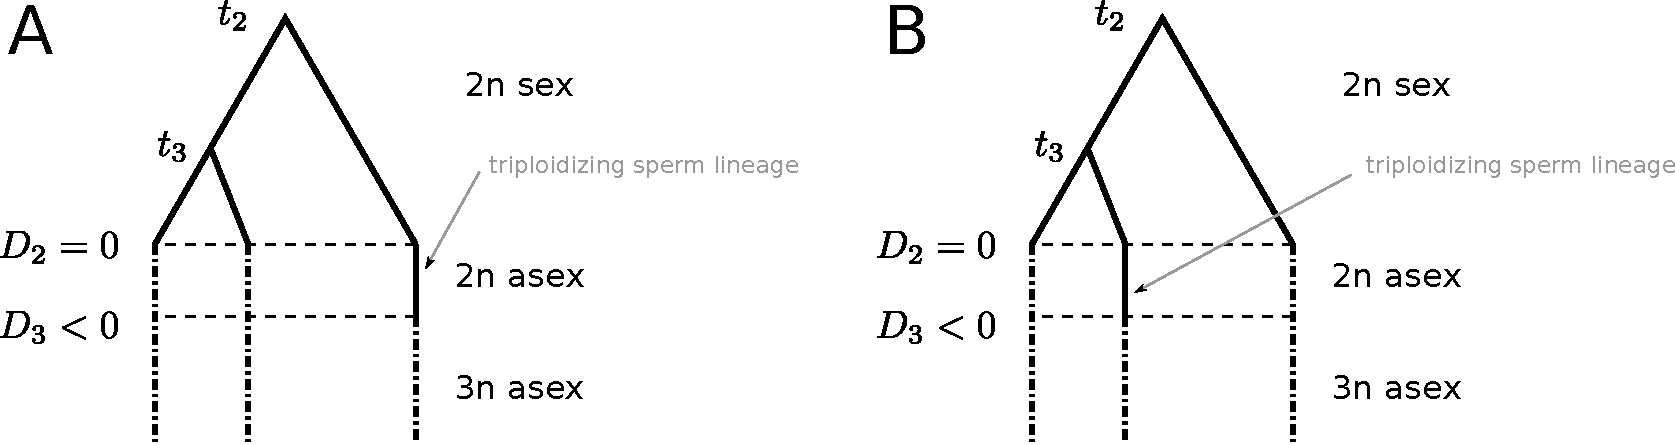
\includegraphics[width=0.8\textwidth]{figs/diptripstate.pdf}
	\caption{
        Figure 1. Two states with the same coalescence times $t_3$ and $t_2$
        but with the triploidizing sperm's lineage subtending a branch that
        coalesceces with the others (in the diploid sexual phase) at $t_2$
        (panel A, $W = 0$) and at $t_3$ (panel B, $W = 1$). $D_2 = 0$ is the
        time of transition to diploid asexuality, and $D_3 < 0$ is the time of
        the transition to triploidy.
    }
    \label{fig:diptripstate}
\end{figure}

\subsection{Diploid-to-triploid transition probabilities --- Summary}

The transition probabilities of the hidden model largely remain the same. A few
changes occur:
\begin{enumerate}
    \item In all previous probabilities, the factor $(2t_2 + t_3)^{-1}$ is
        replaced by the inverse of the new total (sexual) tree length, $(2t_2 +
        t_3 - D_3)^{-1}$, recalling that $D_3 < 0$. These factors are included
        unchanged all the way through the derivations and are still present in
        the final discrete transition probabilities, so they can just be
        replaced with the new factor.
    \item Certain transitions will now change $W$ as well. For example, if
        $W = 0$, (recall, subtending a branch that coalesces at $t_2$), the
        transition $(s_3, s_2) \to (t_3 < s_3, t_2 = s_3)$ implies that now
        $W = 1$.
    \item Additional transition probability must be included, arising from
        recombination events that occur on the triploidizing sperm's sexual
        lineage between $t = D_3$ and $t = 0$.
\end{enumerate}

To do this properly, it will also now be necessary to model the population size
changes that occur in the sexual population during the diploid asexual phase,
since the triploidizing sperm's lineage will experience those demographic
changes. However, the only probabilities that depend on these population sizes
are the ``healing'' probabilities specific to the SMC', meaning that only the
``effective recombination rate'' for this single lineage will depend on this
part of the demographic history. \textbf{For this reason, we will assume that
the diploid sexual population containing the triploidizing sperm is constant in
size.} [This approximation would be unnecessary under the SMC model (vs. the
SMC'), since healing is impossible under the SMC.] It should be a fine
approximation and will have to be tested.

In general, we can expect there to be very little information about the length
of this hypothesized diploid asexual interval in the triploid asexual's
present-day genome. Including this additional period of diploid asexuality
doesn't change the emission probabilities at all; it only changes the
transition probabilities of the hidden model, and these changes seem like they
will be pretty minor. However, it may be possible to rule out long periods of
diploid asexuality in the putatively ancient lineages.

\subsection{Determining when $W$ changes and when it remains the same}

\begin{align}
    \begin{split}
        % case A
        \intertext{For $t_3=s_3;t_2>s_2$:}
        W' &= W\\
        % case B
        \intertext{For $t_3=s_3;t_2<s_2$:}
        W' &= W\\
        % case C
        \intertext{For $t_3<s_3;t_2=s_3$, and $W = 0$:}
        W' &= 1\\
        % case C
        \intertext{For $t_3<s_3;t_2=s_3$, and $W = 1$:}
        W' &= 1 \textrm{ with prob.\ 1/2}\\
        W' &= 0 \textrm{ with prob.\ 1/2}\\
        % case D
        \intertext{For $t_3<s_3; t_2=s_2$:}
        W' = W
        % case E
        \intertext{For $t_3>s_3; t_2=s_2$:}
        W' = W
        % case F
        \intertext{For $t_3=s_2; t_2>s_2, W = 0$:}
        W' = 1\\
        \intertext{For $t_3=s_2; t_2>s_2, W = 1$:}
        W' &= 1 \textrm{ with prob.\ 1/2}\\
        W' &= 0 \textrm{ with prob.\ 1/2}\\
        \intertext{For $t_3=s_3; t_2=s_2$:}
        W' = W\\
    \end{split}
\end{align}

\subsection{Deriving the new probabilities}

The following are the ``supplemental'' probabilities of transition at the site
of a recombination event, due to recombination events happening along the
lineage of the triploidizing sperm in the time interval $(D_3, D_2)$.

% case A
For $t_3=s_3;t_2>s_2$, $W = 0$, and $W' = 0$:
\begin{equation*}
    \int_{D_3}^{0}\frac{du}{2s_2+s_3-D_3}e^{-\Omega(u,0)}e^{-3\Omega(0,s_3)}e^{-2\Omega(s_3,s_2)}\frac{1}{\lambda(t_2)}e^{-\Omega(s_2,t_2)}
\end{equation*}

% case B
For $t_3=s_3;t_2<s_2$, $W = 0$, and $W' = 0$:
\begin{equation*}
    \int_{D_3}^{0}\frac{du}{2s_2+s_3-D_3}e^{-\Omega(u,0)}e^{-3\Omega(0,s_3)}\frac{1}{\lambda(t_2)}e^{-2\Omega(s_3,t_2)}
\end{equation*}

% case C
For $t_3<s_3;t_2=s_3$, $W = 0$, and $W' = 1$:
\begin{equation*}
    \int_{D_3}^{0}\frac{du}{2s_2+s_3-D_3}e^{-\Omega(u,0)}\frac{2}{\lambda(t_3)}e^{-3\Omega(0,t_3)}
\end{equation*}

% case D
For $t_3<s_3; t_2=s_2$, $W = 1$, and $W' = 1$:
\begin{equation*}
    \int_{D_3}^{0}\frac{du}{2s_2+s_3-D_3}e^{-\Omega(u,0)}e^{-3\Omega(0,t_3)}\frac{2}{\lambda(t_3)}
\end{equation*}

% case E
For $t_3>s_3; t_2=s_2$, $W = 1$, $W' = 1$:
\begin{equation*}
    \int_{D_3}^{0}\frac{du}{2s_2+s_3-D_3}e^{-\Omega(u,0)}e^{-3\Omega(0,s_3)}\frac{2}{\lambda(t_3)}e^{-2\Omega(s_3,t_3)}
\end{equation*}

% case F
For $t_3=s_2; t_2>s_2$, $W = 1$, and $W' = 0$:
\begin{equation*}
    \int_{D_3}^{0}\frac{du}{2s_2+s_3-D_3}e^{-\Omega(u,0)}e^{-3\Omega(0,s_3)}e^{-2\Omega(s_3,s_2)}\frac{1}{\lambda(t_2)}e^{-\Omega(s_2,t_2)}
\end{equation*}

\subsection{Calculating discrete transition probabilities with diploid-triploid transition}

Let the relative population size between $D_3$ and $D_2$ be $\lambda_d$.
Replace $s_3$ and $s_2$ with $\E_{i,j}[s_3]$ and $\E_{i,j}[s_2]$, respectively.

\subsubsection{Case A:}
For $i=k< j<l$, ($t_3=s_3\,;t_2>s_2$), $W' = W$:

\begin{align}
    \begin{split}
        &= \frac{2s_2+s_3}{2s_2+s_3-D_3}\,q(i,j,k,l) +\\
        &\qquad
        \delta(W)\frac{1}{2s_2+s_3-D_3}
        \lambda_d\left(1-e^{\frac{D_3}{\lambda_d}}\right)
        e^{-3\Omega(0,s_3)}e^{-2\Omega(s_3,s_2)}\frac{1}{\lambda_l}\int_{T_l}^{T_{l+1}}e^{-\Omega(s_2,t_2)}dt_2\\
        &= \frac{2s_2+s_3}{2s_2+s_3-D_3}\,q(i,j,k,l) +\\
        &\qquad
        \delta(W)\frac{1}{2s_2+s_3-D_3}
        \lambda_d\left(1-e^{\frac{D_3}{\lambda_d}}\right)
        e^{-3\Omega(0,s_3)}e^{-2\Omega(s_3,s_2)}\frac{1}{\lambda_l}e^{-\Omega(s_2,T_l)}\int_{T_l}^{T_{l+1}}e^{-\Omega(T_l,t_2)}dt_2\\
        &= \frac{2s_2+s_3}{2s_2+s_3-D_3}\,q(i,j,k,l) +\\
        &\qquad
        \delta(W)\frac{1}{2s_2+s_3-D_3}
        \lambda_d\left(1-e^{\frac{D_3}{\lambda_d}}\right)
        e^{-3\Omega(0,s_3)}e^{-2\Omega(s_3,s_2)}\frac{1}{\lambda_l}e^{-\Omega(s_2,T_l)}\lambda_l\left(1-e^{-\frac{\Delta_l}{\lambda_l}}\right)\\
        &= \frac{2s_2+s_3}{2s_2+s_3-D_3}\,q(i,j,k,l) +\\
        &\qquad
        \delta(W)\frac{1}{2s_2+s_3-D_3}
        \lambda_d\left(1-e^{\frac{D_3}{\lambda_d}}\right)
        e^{-3\Omega(0,s_3)}e^{-2\Omega(s_3,s_2)}e^{-\Omega(s_2,T_l)}\left(1-e^{-\frac{\Delta_l}{\lambda_l}}\right)\\
    \end{split}
\end{align}
As above we assume that $\Delta_n = \infty$ and thus $e^{-\Delta_n/\lambda_n} = 0$.

\subsubsection{Case B:}
For $i=k<l<j$ ($t_3=s_3; t_2<s_2$) and $W = W'$:

\begin{align}
    \begin{split}
        &= \frac{2s_2+s_3}{2s_2+s_3-D_3}\,q(i,j,k,l) +\\
        &\delta(W)\int_{D_3}^{0}\frac{du}{2s_3+s_2-D_3}e^{-\Omega(u,0)}e^{-3\Omega(0,s_3)}\int_{T_l}^{T_{l+1}}\frac{1}{\lambda(t_2)}e^{-2\Omega(s_3,t_2)}dt_2\\
        &= \frac{2s_2+s_3}{2s_2+s_3-D_3}\,q(i,j,k,l) +\\
        &\delta(W)\frac{1}{2s_2+s_3-D_3}
        \lambda_d\left(1-e^{\frac{D_3}{\lambda_d}}\right)
        e^{-3\Omega(0,s_3)}\frac{1}{\lambda_l}e^{-2\Omega(s_3,T_l)}\int_{T_l}^{T_{l+1}}e^{-2\Omega(T_l,t_2)}dt_2\\
        &= \frac{2s_2+s_3}{2s_2+s_3-D_3}\,q(i,j,k,l) +\\
        &\delta(W)\frac{1}{2s_2+s_3-D_3}
        \lambda_d\left(1-e^{\frac{D_3}{\lambda_d}}\right)
        e^{-3\Omega(0,s_3)}\frac{1}{\lambda_l}e^{-2\Omega(s_3,T_l)}\frac{\lambda_l}{2}\left(1-e^{-\frac{2\Delta_l}{\lambda_l}}\right)\\
        &= \frac{2s_2+s_3}{2s_2+s_3-D_3}\,q(i,j,k,l) +\\
        &\delta(W)\frac{1}{2s_2+s_3-D_3}
        \lambda_d\left(1-e^{\frac{D_3}{\lambda_d}}\right)
        e^{-3\Omega(0,s_3)}e^{-2\Omega(s_3,T_l)}\frac{1}{2}\left(1-e^{-\frac{2\Delta_l}{\lambda_l}}\right)\\
    \end{split}
\end{align}

\subsubsection{Case C}
For $k<i=l<j$ ($t_3<s_3; t_2=s_3$), $W = 0$, $W' = 1$:

\begin{align}
    \begin{split}
        &= \frac{2s_2+s_3}{2s_2+s_3-D_3}\,q(i,j,k,l) +\\
        &\qquad\int_{D_3}^{0}\frac{du}{2s_3+s_2-D_3}e^{-\Omega(u,0)}\int_{T_k}^{T_{k+1}}\frac{2}{\lambda(t_3)}e^{-3\Omega(0,t_3)}dt_3\\
        &= \frac{2s_2+s_3}{2s_2+s_3-D_3}\,q(i,j,k,l) +\\
        &\qquad\frac{\lambda_d\left(1-e^{\frac{D_3}{\lambda_d}}\right)}{2s_2+s_3-D_3}
        \frac{2}{\lambda_k}e^{-3\Omega(0,T_k)}\int_{T_k}^{T_{k+1}}e^{-3\Omega(T_k,t_3)}dt_3\\
        &= \frac{2s_2+s_3}{2s_2+s_3-D_3}\,q(i,j,k,l) +\\
        &\qquad\frac{\lambda_d\left(1-e^{\frac{D_3}{\lambda_d}}\right)}{2s_2+s_3-D_3}
        \frac{2}{\lambda_k}e^{-3\Omega(0,T_k)}\frac{\lambda_k}{3}\left(1-e^{-\frac{3\Delta_k}{\lambda_k}}\right)\\
        &= \frac{2s_2+s_3}{2s_2+s_3-D_3}\,q(i,j,k,l) +\\
        &\qquad\frac{\lambda_d\left(1-e^{\frac{D_3}{\lambda_d}}\right)}{2s_2+s_3-D_3}
        \frac{2}{3}e^{-3\Omega(0,T_k)}\left(1-e^{-\frac{3\Delta_k}{\lambda_k}}\right)\\
    \end{split}
\end{align}

For $k<i=l<j$ ($t_3<s_3; t_2=s_3$), $W = 1$, $W' \in \{0,1\}$:

\begin{align}
    \begin{split}
        &= \frac{1}{2}\frac{2s_2+s_3}{2s_2+s_3-D_3}\,q(i,j,k,l)
    \end{split}
\end{align}

\subsubsection{Case D}
For $k<i< j=l$ ($t_3<s_3; t_2=s_2$) and $W' = W$:

\begin{align}
    \begin{split}
        &= \frac{2s_2+s_3}{2s_2+s_3-D_3}\,q(i,j,k,l) +\\
        &\qquad
        \delta(W-1)\int_{D_3}^{0}\frac{du}{2s_3+s_2-D_3}e^{-\Omega(u,0)}\int_{T_k}^{T_{k+1}}e^{-3\Omega(0,t_3)}\frac{2}{\lambda(t_3)}dt_3\\
        &= \frac{2s_2+s_3}{2s_2+s_3-D_3}\,q(i,j,k,l) +\\
        &\qquad
        \delta(W-1)\frac{\lambda_d\left(1-e^{\frac{D_3}{\lambda_d}}\right)}{2s_2+s_3-D_3}\frac{2}{\lambda_k}e^{-3\Omega(0,T_k)}\int_{T_k}^{T_{k+1}}e^{-3\Omega(T_k,t_3)}dt_3\\
        &= \frac{2s_2+s_3}{2s_2+s_3-D_3}\,q(i,j,k,l) +\\
        &\qquad
        \delta(W-1)\frac{\lambda_d\left(1-e^{\frac{D_3}{\lambda_d}}\right)}{2s_2+s_3-D_3}\frac{2}{\lambda_k}e^{-3\Omega(0,T_k)}\frac{\lambda_k}{3}\left(1-e^{-\frac{3\Delta_k}{\lambda_k}}\right)\\
        &= \frac{2s_2+s_3}{2s_2+s_3-D_3}\,q(i,j,k,l) +\\
        &\qquad
        \delta(W-1)\frac{\lambda_d\left(1-e^{\frac{D_3}{\lambda_d}}\right)}{2s_2+s_3-D_3}\frac{2}{3}e^{-3\Omega(0,T_k)}\left(1-e^{-\frac{3\Delta_k}{\lambda_k}}\right)\\
    \end{split}
\end{align}

\subsubsection{Case E}
For $i<k<j=l$ ($t_3>s_3; t_2=s_2$) and $W' = W$:

\begin{align}
    \begin{split}
        &= \frac{2s_2+s_3}{2s_2+s_3-D_3}\,q(i,j,k,l) +\\
        &\qquad
        \delta(W = 1)\int_{D_3}^{0}\frac{du}{2s_3+s_2-D_3}e^{-\Omega(u,0)}e^{-3\Omega(0,s_3)}\int_{T_k}^{T_{k+1}}\frac{2}{\lambda(t_3)}e^{-2\Omega(s_3,t_3)}dt_3\\
        &= \frac{2s_2+s_3}{2s_2+s_3-D_3}\,q(i,j,k,l) +\\
        &\qquad
        \delta(W-1)\frac{\lambda_d\left(1-e^{\frac{D_3}{\lambda_d}}\right)}{2s_2+s_3-D_3}
        e^{-3\Omega(0,s_3)}\frac{2}{\lambda_k}e^{-2\Omega(s_3,T_k)}\frac{\lambda_k}{2}\left(1-e^{-\frac{2\Delta_k}{\lambda_k}}\right)\\
        &= \frac{2s_2+s_3}{2s_2+s_3-D_3}\,q(i,j,k,l) +\\
        &\qquad
        \delta(W-1)\frac{\lambda_d\left(1-e^{\frac{D_3}{\lambda_d}}\right)}{2s_2+s_3-D_3}
        e^{-3\Omega(0,s_3)}e^{-2\Omega(s_3,T_k)}\left(1-e^{-\frac{2\Delta_k}{\lambda_k}}\right)\\
    \end{split}
\end{align}

\subsubsection{Case F}
For $i<j=k<l$ ($t_3=s_2; t_2>s_2$) and $W = 1$:

\begin{align}
    \begin{split}
        &= \frac{2s_2+s_3}{2s_2+s_3-D_3}\frac{1}{2}\,q(i,j,k,l) +\\
        &\qquad\delta(W')
        \int_{D_3}^{0}\frac{du}{2s_3+s_2-D_3}e^{-\Omega(u,0)}e^{-3\Omega(0,s_3)}e^{-2\Omega(s_3,s_2)}\int_{T_l}^{T_{l+1}}\frac{1}{\lambda(t_2)}e^{-\Omega(s_2,t_2)}dt_2\\
        &= \frac{2s_2+s_3}{2s_2+s_3-D_3}\frac{1}{2}\,q(i,j,k,l) +\\
        &\qquad\delta(W')
        \frac{\lambda_d\left(1-e^{\frac{D_3}{\lambda_d}}\right)}{2s_2+s_3-D_3}e^{-3\Omega(0,s_3)}e^{-2\Omega(s_3,s_2)}\frac{1}{\lambda_l}e^{-\Omega(s_2,T_l)}\int_{T_l}^{T_{l+1}}e^{-\Omega(T_l,t_2)}dt_2\\
        &= \frac{2s_2+s_3}{2s_2+s_3-D_3}\frac{1}{2}\,q(i,j,k,l) +\\
        &\qquad\delta(W')
        \frac{\lambda_d\left(1-e^{\frac{D_3}{\lambda_d}}\right)}{2s_2+s_3-D_3}e^{-3\Omega(0,s_3)}e^{-2\Omega(s_3,s_2)}\frac{1}{\lambda_l}e^{-\Omega(s_2,T_l)}\lambda_l\left(1-e^{-\frac{\Delta_l}{\lambda_l}}\right)\\
        &= \frac{2s_2+s_3}{2s_2+s_3-D_3}\frac{1}{2}\,q(i,j,k,l) +\\
        &\qquad\delta(W')
        \frac{\lambda_d\left(1-e^{\frac{D_3}{\lambda_d}}\right)}{2s_2+s_3-D_3}e^{-3\Omega(0,s_3)}e^{-2\Omega(s_3,s_2)}e^{-\Omega(s_2,T_l)}\left(1-e^{-\frac{\Delta_l}{\lambda_l}}\right)\\
    \end{split}
\end{align}

For $i<j=k<l$ ($t_3=s_2; t_2>s_2$) and $W = 0$, $W' = 1$:

\begin{align}
    \begin{split}
        &= \frac{2s_2+s_3}{2s_2+s_3-D_3}\,q(i,j,k,l)
    \end{split}
\end{align}

\subsubsection{Case G}
For $i=k=l<j$ and $t_3=s_3; t_2<s_2$ and $W = W'$:

\begin{align}
    \begin{split}
        &= \frac{2s_2+s_3}{2s_2+s_3-D_3}\,q^{G}(i,j,k,l)+\\
        &\qquad
        \delta(W)
        \int_{D_3}^{0}\frac{du}{2s_3+s_2-D_3}e^{-\Omega(u,0)}e^{-3\Omega(0,s_3)}\int_{s_3}^{T_{l+1}}\frac{1}{\lambda(t_2)}e^{-2\Omega(s_3,t_2)}dt_2\\
        &= \frac{2s_2+s_3}{2s_2+s_3-D_3}\,q^{G}(i,j,k,l)+\\
        &\qquad
        \delta(W)
        \frac{\lambda_d\left(1-e^{\frac{D_3}{\lambda_d}}\right)}{2s_2+s_3-D_3}e^{-3\Omega(0,s_3)}\frac{1}{\lambda_l}\int_{s_3}^{T_{l+1}}e^{-2\Omega(s_3,t_2)}dt_2\\
        &= \frac{2s_2+s_3}{2s_2+s_3-D_3}\,q^{G}(i,j,k,l)+\\
        &\qquad
        \delta(W)
        \frac{\lambda_d\left(1-e^{\frac{D_3}{\lambda_d}}\right)}{2s_2+s_3-D_3}e^{-3\Omega(0,s_3)}\frac{1}{\lambda_l}\frac{\lambda_l}{2}\left(1-e^{-\frac{2(T_{l+1}-s_3)}{\lambda_l}}\right)\\
        &= \frac{2s_2+s_3}{2s_2+s_3-D_3}\,q^{G}(i,j,k,l)+\\
        &\qquad
        \delta(W)
        \frac{\lambda_d\left(1-e^{\frac{D_3}{\lambda_d}}\right)}{2s_2+s_3-D_3}e^{-3\Omega(0,s_3)}\frac{1}{2}\left(1-e^{-\frac{2(T_{l+1}-s_3)}{\lambda_l}}\right)\\
    \end{split}
\end{align}
Here, $q^G(i,j,k,l)$ is case G without the diploid-to-triploid variables.

\subsubsection{Case G2}
For $i=k=l<j$ and $t_3<s_3;t_2=s_3$, $W = 0$, and $W' = 1$:

\begin{align}
    \begin{split}
        &= \frac{2s_2+s_3}{2s_2+s_3-D_3}\,q^{G2}(i,j,k,l)+\\
        &\qquad
        \int_{D_3}^{0}\frac{du}{2s_3+s_2-D_3}e^{-\Omega(u,0)}\int_{T_k}^{s_3}\frac{2}{\lambda(t_3)}e^{-3\Omega(0,t_3)}dt_3\\
        &= \frac{2s_2+s_3}{2s_2+s_3-D_3}\,q^{G2}(i,j,k,l)+\\
        &\qquad
        \frac{\lambda_d\left(e^{-\frac{D_3}{\lambda_d}}-1\right)}{2s_2+s_3-D_3}\frac{2}{\lambda_k}e^{-3\Omega(0,T_k)}\int_{T_k}^{s_3}e^{-3\Omega(T_k,t_3)}dt_3\\
        &= \frac{2s_2+s_3}{2s_2+s_3-D_3}\,q^{G2}(i,j,k,l)+\\
        &\qquad
        \frac{\lambda_d\left(1-e^{\frac{D_3}{\lambda_d}}\right)}{2s_2+s_3-D_3}\frac{2}{\lambda_k}e^{-3\Omega(0,T_k)}\frac{\lambda_k}{3}\left(1-e^{-\frac{3(s_3-T_k)}{\lambda_k}}\right)\\
        &= \frac{2s_2+s_3}{2s_2+s_3-D_3}\,q^{G2}(i,j,k,l)+\\
        &\qquad
        \frac{\lambda_d\left(1-e^{\frac{D_3}{\lambda_d}}\right)}{2s_2+s_3-D_3}\frac{2}{3}e^{-3\Omega(0,T_k)}\left(1-e^{-\frac{3(s_3-T_k)}{\lambda_k}}\right)\\
    \end{split}
\end{align}

For $t_3<s_3;t_2=s_3$, $W = 1$, $W' \in \{0,1\}$:
\begin{align}
    \begin{split}
        &= \frac{1}{2}\frac{2s_2+s_3}{2s_2+s_3-D_3}\,q^{G2}(i,j,k,l)\\
    \end{split}
\end{align}

\subsubsection{Case H}
For $i<k=l=j$ ($t_3>s_3\,;t_2=s_2$) and $W = W'$:
\begin{align}
    \begin{split}
        &= \frac{2s_2+s_3}{2s_2+s_3-D_3}\,q^{H}(i,j,k,l)+\\
        &\qquad
        \delta(W-1)\int_{D_3}^{0}\frac{du}{2s_3+s_2-D_3}e^{-\Omega(u,0)}e^{-3\Omega(0,s_3)}\int_{T_k}^{s_2}\frac{2}{\lambda(t_3)}e^{-2\Omega(s_3,t_3)}dt_3\\
        &= \frac{2s_2+s_3}{2s_2+s_3-D_3}\,q^{H}(i,j,k,l)+\\
        &\qquad
        \delta(W-1)\frac{\lambda_d\left(1-e^{\frac{D_3}{\lambda_d}}\right)}{2s_2+s_3-D_3}e^{-3\Omega(0,s_3)}\frac{2}{\lambda_k}e^{-2\Omega(s_3,T_k)}\int_{T_k}^{s_2}e^{-2\Omega(T_k,t_3)}dt_3\\
        &= \frac{2s_2+s_3}{2s_2+s_3-D_3}\,q^{H}(i,j,k,l)+\\
        &\qquad
        \delta(W-1)\frac{\lambda_d\left(1-e^{\frac{D_3}{\lambda_d}}\right)}{2s_2+s_3-D_3}e^{-3\Omega(0,s_3)}\frac{2}{\lambda_k}e^{-2\Omega(s_3,T_k)}\frac{\lambda_k}{2}\left(1-e^{-\frac{2(s_2-T_k)}{\lambda_k}}\right)\\
        &= \frac{2s_2+s_3}{2s_2+s_3-D_3}\,q^{H}(i,j,k,l)+\\
        &\qquad
        \delta(W-1)\frac{\lambda_d\left(1-e^{\frac{D_3}{\lambda_d}}\right)}{2s_2+s_3-D_3}e^{-3\Omega(0,s_3)}e^{-2\Omega(s_3,T_k)}\left(1-e^{-\frac{2(s_2-T_k)}{\lambda_k}}\right)\\
    \end{split}
\end{align}

\subsubsection{Case H2}

For $i<k=l=j$ and $t_3=s_2\,;t_2>s_2$, $W = 0$, $W' = 1$:
\begin{align}
    \begin{split}
        &= \frac{2s_2+s_3}{2s_2+s_3-D_3}\,q^{H2}(i,j,k,l)
    \end{split}
\end{align}

For $i<k=l=j$ and $t_3=s_2\,;t_2>s_2$, $W = 1$, $W' \in \{0,1\}$:
\begin{align}
    \begin{split}
        &= \frac{1}{2}\frac{2s_2+s_3}{2s_2+s_3-D_3}\,q^{H2}(i,j,k,l)+\\
        &\qquad
        \delta(W')\int_{D_3}^{0}\frac{du}{2s_3+s_2-D_3}e^{-\Omega(u,0)}e^{-3\Omega(0,s_3)}e^{-2\Omega(s_3,s_2)}\int_{s_2}^{T_{l+1}}\frac{1}{\lambda(t_2)}e^{-\Omega(s_2,t_2)}dt_2\\
        &= \frac{1}{2}\frac{2s_2+s_3}{2s_2+s_3-D_3}\,q^{H2}(i,j,k,l)+\\
        &\qquad
        \delta(W')\frac{\lambda_d\left(1-e^{\frac{D_3}{\lambda_d}}\right)}{2s_2+s_3-D_3}e^{-3\Omega(0,s_3)}e^{-2\Omega(s_3,s_2)}
        \frac{1}{\lambda_l}\int_{s_2}^{T_{l+1}}e^{-\Omega(s_2,t_2)}dt_2\\
        &= \frac{1}{2}\frac{2s_2+s_3}{2s_2+s_3-D_3}\,q^{H2}(i,j,k,l)+\\
        &\qquad
        \delta(W')\frac{\lambda_d\left(1-e^{\frac{D_3}{\lambda_d}}\right)}{2s_2+s_3-D_3}e^{-3\Omega(0,s_3)}e^{-2\Omega(s_3,s_2)}
        \frac{1}{\lambda_l}\lambda_l\left(1-e^{-\frac{T_{l+1}-s_2}{\lambda_l}}\right)\\
        &= \frac{1}{2}\frac{2s_2+s_3}{2s_2+s_3-D_3}\,q^{H2}(i,j,k,l)+\\
        &\qquad
        \delta(W')\frac{\lambda_d\left(1-e^{\frac{D_3}{\lambda_d}}\right)}{2s_2+s_3-D_3}e^{-3\Omega(0,s_3)}e^{-2\Omega(s_3,s_2)}
        \left(1-[1-\delta(l-n)]e^{-\frac{T_{l+1}-s_2}{\lambda_l}}\right)\\
    \end{split}
\end{align}

\subsubsection{Case I}
For $i=j=k<l$ and $t_3=s_3;t_2>s_2$, $W' = W$:


\begin{align}
    \begin{split}
        &= \frac{2s_2+s_3}{2s_2+s_3-D_3}\,q^{(I)}(i,j,k,l)+\\
        &\qquad \delta(W)
        \int_{D_3}^{0}\frac{1}{2s_3+s_2-D_3}e^{-\Omega(u,0)}e^{-3\Omega(0,s_3)}e^{-2\Omega(s_3,s_2)}
        \int_{T_l}^{T_{l+1}}\frac{1}{\lambda(t_2)}e^{-\Omega(s_2,t_2)}dt_2\\
        &= \frac{2s_2+s_3}{2s_2+s_3-D_3}\,q^{(I)}(i,j,k,l)+\\
        &\qquad \delta(W)
        \frac{\lambda_d\left(1-e^{\frac{D_3}{\lambda_d}}\right)}{2s_2+s_3-D_3}e^{-3\Omega(0,s_3)}e^{-2\Omega(s_3,s_2)}
        \frac{1}{\lambda_l}e^{-\Omega(s_2,T_l)}\int_{T_l}^{T_{l+1}}e^{-\Omega(T_l,t_2)}dt_2\\
        &= \frac{2s_2+s_3}{2s_2+s_3-D_3}\,q^{(I)}(i,j,k,l)+\\
        &\qquad \delta(W)
        \frac{\lambda_d\left(1-e^{\frac{D_3}{\lambda_d}}\right)}{2s_2+s_3-D_3}e^{-3\Omega(0,s_3)}e^{-2\Omega(s_3,s_2)}
        \frac{1}{\lambda_l}e^{-\Omega(s_2,T_l)}\lambda_l\left(1-e^{-\frac{\Delta_l}{\lambda_l}}\right)\\
        &= \frac{2s_2+s_3}{2s_2+s_3-D_3}\,q^{(I)}(i,j,k,l)+\\
        &\qquad \delta(W)
        \frac{\lambda_d\left(1-e^{\frac{D_3}{\lambda_d}}\right)}{2s_2+s_3-D_3}e^{-3\Omega(0,s_3)}e^{-2\Omega(s_3,s_2)}
        e^{-\Omega(s_2,T_l)}\left(1-e^{-\frac{\Delta_l}{\lambda_l}}\right)\\
    \end{split}
\end{align}

\subsubsection{Case I2}
For $i=j=k<l$ and $t_3=s_2;t_2>s_2$, $W = 0$, $W' = 1$:

\begin{align}
    \begin{split}
        &= \frac{2s_2+s_3}{2s_2+s_3-D_3}\,q^{I2}(i,j,k,l)\\
    \end{split}
\end{align}

For $i=j=k<l$ and $t_3=s_2;t_2>s_2$, $W = 1$, $W' \in \{0,1\}$:

\begin{align}
    \begin{split}
        &= \frac{1}{2}\frac{2s_2+s_3}{2s_2+s_3-D_3}q^{I2}(i,j,k,l)+\\
        &\qquad \delta(W')
        \int_{D_3}^{0}\frac{du}{2s_3+s_2-D_3}e^{-\Omega(u,0)}e^{-3\Omega(0,s_3)}e^{-2\Omega(s_3,s_2)}\int_{T_l}^{T_{l+1}}\frac{1}{\lambda(t_2)}e^{-\Omega(s_2,t_2)}dt_2\\
        &= \frac{1}{2}\frac{2s_2+s_3}{2s_2+s_3-D_3}q^{I2}(i,j,k,l)+\\
        &\qquad \delta(W')
        \frac{\lambda_d\left(1-e^{\frac{D_3}{\lambda_d}}\right)}{2s_2+s_3-D_3}e^{-3\Omega(0,s_3)}e^{-2\Omega(s_3,s_2)}\frac{1}{\lambda_l}e^{-\Omega(s_2,T_l)}\int_{T_l}^{T_{l+1}}e^{-\Omega(T_l,t_2)}dt_2\\
        &= \frac{1}{2}\frac{2s_2+s_3}{2s_2+s_3-D_3}q^{I2}(i,j,k,l)+\\
        &\qquad \delta(W')
        \frac{\lambda_d\left(1-e^{\frac{D_3}{\lambda_d}}\right)}{2s_2+s_3-D_3}e^{-3\Omega(0,s_3)}e^{-2\Omega(s_3,s_2)}\frac{1}{\lambda_l}e^{-\Omega(s_2,T_l)}\lambda_l\left(1-e^{-\frac{\Delta_l}{\lambda_l}}\right)\\
        &= \frac{1}{2}\frac{2s_2+s_3}{2s_2+s_3-D_3}q^{I2}(i,j,k,l)+\\
        &\qquad \delta(W')
        \frac{\lambda_d\left(1-e^{\frac{D_3}{\lambda_d}}\right)}{2s_2+s_3-D_3}e^{-3\Omega(0,s_3)}e^{-2\Omega(s_3,s_2)}e^{-\Omega(s_2,T_l)}\left(1-e^{-\frac{\Delta_l}{\lambda_l}}\right)\\
    \end{split}
\end{align}

\subsubsection{Case J}
For $k<i=j=l$ and $t_3<s_3;t_2=s_2$, $W' = W$:
\begin{align}
    \begin{split}
        &=\frac{2s_2+s_3}{2s_2+s_3-D_3}q^{J}(i,j,k,l)+
        \delta(W-1)
        \int_{D_3}^{0}\frac{du}{2s_3+s_2-D_3}e^{-\Omega(u,0)}\frac{2}{\lambda_k}e^{-3\Omega(0,T_k)}\int_{T_k}^{T_{k+1}}e^{-3\Omega(T_k,t_3)}dt_3\\
        &=\frac{2s_2+s_3}{2s_2+s_3-D_3}q^{J}(i,j,k,l)+
        \delta(W-1)
        \frac{\lambda_d\left(1-e^{\frac{D_3}{\lambda_d}}\right)}{2s_2+s_3-D_3}\frac{2}{\lambda_k}e^{-3\Omega(0,T_k)}\frac{\lambda_k}{3}\left(1-e^{-\frac{3\Delta_k}{\lambda_k}}\right)\\
        &=\frac{2s_2+s_3}{2s_2+s_3-D_3}q^{J}(i,j,k,l)+
        \delta(W-1)
        \frac{\lambda_d\left(1-e^{\frac{D_3}{\lambda_d}}\right)}{2s_2+s_3-D_3}\frac{2}{3}e^{-3\Omega(0,T_k)}\left(1-e^{-\frac{3\Delta_k}{\lambda_k}}\right)\\
    \end{split}
\end{align}

\subsubsection{Case J2}
For $k<i=j=l$ and $t_3<s_3;t_2=s_3$, $W = 0$, $W' = 1$:
\begin{align}
    \begin{split}
        &=\frac{2s_2+s_3}{2s_2+s_3-D_3}q^{J2}(i,j,k,l)+\int_{D_3}^{0}\frac{du}{2s_3+s_2-D_3}e^{-\Omega(u,0)}\int_{T_k}^{T_{k+1}}\frac{2}{\lambda(t_3)}e^{-3\Omega(0,t_3)}dt_3\\
        &=\frac{2s_2+s_3}{2s_2+s_3-D_3}q^{J2}(i,j,k,l)+\frac{\lambda_d\left(1-e^{\frac{D_3}{\lambda_d}}\right)}{2s_2+s_3-D_3}\frac{2}{\lambda_k}e^{-3\Omega(0,T_k)}\int_{T_k}^{T_{k+1}}e^{-3\Omega(T_k,t_3)}dt_3\\
        &=\frac{2s_2+s_3}{2s_2+s_3-D_3}q^{J2}(i,j,k,l)+\frac{\lambda_d\left(1-e^{\frac{D_3}{\lambda_d}}\right)}{2s_2+s_3-D_3}\frac{2}{\lambda_k}e^{-3\Omega(0,T_k)}\frac{\lambda_k}{3}\left(1-e^{-\frac{3\Delta_k}{\lambda_k}}\right)\\
        &=\frac{2s_2+s_3}{2s_2+s_3-D_3}q^{J2}(i,j,k,l)+\frac{\lambda_d\left(1-e^{\frac{D_3}{\lambda_d}}\right)}{2s_2+s_3-D_3}\frac{2}{3}e^{-3\Omega(0,T_k)}\left(1-e^{-\frac{3\Delta_k}{\lambda_k}}\right)\\
    \end{split}
\end{align}

For $k<i=j=l$ and $t_3<s_3;t_2=s_3$, $W = 1$, $W' \in \{0,1\}$:
\begin{align}
    \begin{split}
        &=\frac{1}{2}\frac{2s_2+s_3}{2s_2+s_3-D_3}q^{J2}(i,j,k,l)
    \end{split}
\end{align}

(Double-checked these.)

\section{Harris et al.\ algorithm for triploid genealogy}

Define $f(x_{1:l}, j)$ as the joint forward probability of observing the
partial emitted sequence $x_{1:l} = x_1, \dots, x_l$ and the hidden state
(coalescence time) $T_l = j$ at locus $l$. Let the number of discretized time
intervals be $d$, and define $\phi(j \mid k)$ as $\Prob(T_{l+1} = j \mid T_l =
k)$.

\begin{equation}
    f(x_{1:l+1}, j) = \xi(x_{l+1} \mid j)
        \sum_{k=1}^d f(x_{1:l}, k)\phi(j\mid k),
    \label{eq:harrisforward}
\end{equation}
which contains $d$ terms. Since there are $d$ possibilities for $j$, the
algorithm should take $O(d^2L)$ time to compute.

Decompose the transition from $l$ to $l+1$ as a sequence of component events.
Let $R_i$ be the event that a recombination event occurs during time interval
$i$, and let $\bar{R}$ be the event that no recombination occurs. Then

\begin{equation}
    \phi(j \mid k) = \sum_{i=1}^{\min(j,k)}
        \Prob(R_i, T_{l+1} = j \mid T_l = k)
            + \ind_{j=k}\Prob(\bar{R} \mid T_l = k)
    \label{eq:pcoalsumrecomb}
\end{equation}

Two events: $C_{>i}$ denotes the event where the recombination event occurs at
or before $i$ and floats into $i+1$, and $C_i$ denotes the event where the
recombined lineage coalesces back in interval $i$. Note that $\Prob(R_i, C_i
\mid T_l = i')$ is independent of $i'$ whenever $i < i'$. (Still working
between $l$ and $l+1$, here.) This is also true of $\Prob(R_i, C_{>i} \mid T_l
= i')$. Then we can write

\begin{equation}
    \Prob(R_i, T_{l+1} = j \mid T_l = k) = 
    \begin{cases}
        \Prob(R_i,C_i \mid T_l = i),&i=j=k \\
        \Prob(R_i, C_i \mid T_l > i),&i = j < k \\
        \Prob(R_i, C_{>i} \mid T_l = i) \Prob(C_j \mid C_{>j-1})
            \prod_{m=i}^{j-1}\Prob(C_{>k'+1} \mid C_{>k'}),&i=k<j \\
        \Prob(R_i, C_{>i} \mid T_l > i)\Prob(C_j \mid C_{>j-1})
            \prod_{k'=i}^{j-1}\Prob(C_{>k'+1} \mid C_{>k'}), &i < \min(j,k)
    \end{cases}
    \label{eq:recombcases}
\end{equation}

By combining \eqref{eq:pcoalsumrecomb} and \eqref{eq:recombcases}, we can
remove the sum over $T_l = k$ in computing $f(x_{1:l+1}, j)$. Define the
additional forward probabilities

\begin{equation}
    f(x_{1:l},T_l=k) := \Prob(x_{1:l}, T_l = k)
\end{equation}

\begin{equation}
    f(x_{1:l}, T_l > k) := \Prob(x_{1:l}, T_l > k) = 
        \sum_{k'=k+1}^d f(x_{1:l}, T_l = k)
\end{equation}

\begin{align}
    \begin{split}
        f(x_{1:l}, R_{\le j}, C_{>j}) := &
            \sum_{i=1}^j\Prob(x_{1:l}, R_i, C_{>i}, \dots, C_{>j}) \\
            &= \sum_{i=1}^j \bigg\{
                \prod_{i'=i+1}^j\Prob(C_{>i'} \mid C_{>i'-1})
             \\
            &\times \big[ f(x_{1:l}, T_l = i)\Prob(R_i,C_{>i}\mid T_l = i) +
                f(x_{1:l},T_l>i)\Prob(R_i, C_{>i} | T_l > i) \big] \bigg\}.
    \end{split}
\end{align}

Then \eqref{eq:harrisforward} can be written as

\begin{align}
    \begin{split}
        f(x_{1:l+1},j) &= \xi(x_{l+1} \mid j) \\
    & \times \bigg[ f(x_{1:l},
        R_{\le j-1}, C_{>j-1})\Prob(C_j \mid C_{>j-1}) + f(x_{1:l},T_l >
        j)\Prob(R_j, C_j \mid T_l > j) + \\
        &\qquad f(x_{1:l}, T_l = j) \Prob(R_j, C_j
    \mid T_l = j) + f(x_{1:l}, j) \Prob(\bar{R} \mid T_l = j) \bigg].
    \end{split}
\end{align}

\section{Genotype likelihoods and emission probabilities}

When using observed genotypes, the emissions probability, given the hidden
state $(t_3, t_2)$ (with $T_d$), is

\begin{equation}
    P_e(G) = e_G(t_3, t_2, t_d) = 
    \begin{cases}
        e^{-\frac{\theta b \left(2t_2+t_3+3T_d\right)}{2}}&G=0\\
        e^{-\frac{\theta b \left(t_2-t_3\right)}{2}}\left(1-e^{-\frac{\theta b \left(2t_3+t_2+3T_d\right)}{2}}\right)&G=1\\
        \left(1-e^{-\frac{\theta b \left(t_2-t_3\right)}{2}}\right)e^{-\frac{\theta b \left(2t_3+t_2+3T_d\right)}{2}}&G=2\\
        \left(1-e^{-\frac{\theta b \left(t_2-t_3\right)}{2}}\right)\left(1-e^{-\frac{\theta b \left(2t_3+t_2+3T_d\right)}{2}}\right)&G=3.
    \label{eq:emissionprobs2}
    \end{cases}
\end{equation}

(Using Vladimir's equations and notation...) Given a window of base pairs
$\nu$, with reads $S^{(\nu)}$ covering that window, we want $P_e(\nu)$, the
emission probability of the reads in that window. This is 

\begin{equation}
    P_e(\nu) = P(S^{(\nu)} \mid T) = \prod_{i \in \nu}P(S_i^{(\nu)} \mid T) = 
    \prod_{i \in \nu}\sum_{G_i} P(S_i^{(\nu)} \mid G_i)P(G_i \mid T),
\end{equation}
where $S_i^{(\nu)}$ is the set of reads in the $i$th window in window $\nu$.
Here, $T$ is the hidden state $(t_3, t_2, T_d)$, and $P(G_i \mid T) = e_G(t_3,
t_2, T_d)$. 

\section{GATK likelihoods for triploids}

For each base quality phred score $i \in 0, \dots, 256$, the probability of an
accurate base call is $1-10^{-i/10}$, and the probability of an error is
$(10^{-i/10})/3$ for each base other than the best. Given genotype $G = \{A_1,
A_2, A_3\}$,

\begin{equation}
    P(D \mid G) = \prod_{b \in \textrm{pileup}} P(b \mid G),
\end{equation}


\begin{equation}
    P(b \mid G) = \frac{1}{3}P(b \mid A_1) + \frac{1}{3}P(b \mid A_2) + 
        \frac{1}{3}P(b \mid A_3),
\end{equation}
and

\begin{equation}
    P(b \mid A) =
    \begin{cases}
        1-10^{-q_b/10}&b =A\\
        \frac{10^{-q_b/10}}{3}& b \neq a
    \end{cases}
\end{equation}

A (log) likelihood needs to be calculated for each of the 20 genotypes.

\end{document}
